\makeatletter
\def\input@path{{libs/}}
\makeatother
\documentclass[bcl,numbers]{coppe}

\usepackage[utf8]{inputenc}
\usepackage{etoolbox}
\usepackage{amsmath}
\usepackage{amsthm}
\usepackage{amscd}
\usepackage{amsfonts}
\usepackage{mathrsfs}
\usepackage[dvipsnames]{xcolor}
\usepackage{enumerate}
\usepackage{hyperref}
\usepackage[all]{xy}
\usepackage[style=long]{glossaries-extra}
\usepackage{pst-node}
\usepackage{tikz-cd}
\usepackage{tikz}
\usepackage{caption}
\usepackage{subcaption}
\usepackage{float}
\usetikzlibrary{calc}
\usepackage{fancyhdr}
\usepackage{etoolbox}
\usepackage{pdfpages}
\usetikzlibrary{arrows}
\usepackage{indentfirst}
\usepackage{comment}
\usepackage{multicol}
\usepackage{float}
\usepackage{wrapfig}%d
\usepackage{xcolor}
\usepackage{soul} % Para \hl
\usepackage{todonotes}
\usepackage{algorithm}
\usepackage{algpseudocode}
\usepackage{booktabs}

\definecolor{mygreen}{rgb}{0, 0.3, 0}
\definecolor{myred}{rgb}{0.4,0,0}

\hypersetup{
     colorlinks=true,
     linkcolor=black,
     filecolor=black,
     citecolor=black,
     urlcolor=black,
}

\sloppy
\hyphenpenalty=100000
\clubpenalty=10000
\widowpenalty=10000
\displaywidowpenalty=10000

\geometry{top=35mm, bottom=25mm, left=40mm, right=25mm}
\parindent=15mm
\linespread{1.5}


\begin{comment}
    \parindent=15mm

\geometry{paperwidth=210mm,paperheight=297mm,
textwidth=150mm,textheight=210mm,
top=35mm,bottom=25mm,
left=40mm,right=25mm}

\linespread{1.5}
\end{comment}

\theoremstyle{plain}
\newtheorem{teo}{Teorema}[section]
\newtheorem{lema}{Lema}[section]
\newtheorem{prop}{Proposição}[section]
\newtheorem{coro}{Corolário}[section]
\newtheorem{afirm}{Afirmação}[section]
\newtheorem*{tfa}{Teorema Fundamental da Álgebra}
\newtheorem*{corolario}{Corolário}

\theoremstyle{definition}
\newtheorem{df}{Definição}[section]
\newtheorem{ex}{Exemplo}[section]
\newtheorem{prova}{Prova}[section]
\patchcmd{\quote}{\rightmargin}{\leftmargin 4cm \rightmargin 0}{}{}
% ======= Anotações e marcações ===========
\usepackage{xcolor}
\usepackage{todonotes} % para comentários visuais na margem

% Comandos personalizados para comentários
\newcommand{\TODO}[1]{\todo[inline,color=yellow!90!white]{TODO: #1}}          % Amarelo claro yellow!20!white
\newcommand{\FIXME}[1]{\todo[inline,color=orange!30!white]{FIXME: #1}}         % Laranja claro orange!30!white
\newcommand{\NOTE}[1]{\todo[inline,color=green!20!white]{NOTE: #1}}        % Verde claro green!20!white
\newcommand{\HACK}[1]{\todo[inline,color=purple!20!white]{HACK: #1}}        % Roxo claro purple!20!white
\newcommand{\BUG}[1]{\todo[inline,color=red!30!white]{BUG: #1}}          % Vermelho claro red!30!white

% Comentários por autor
\newcommand{\EnzoR}[1]{\todo[inline,color=violet!20!white]{@EnzoR: #1}}
\newcommand{\LucasM}[1]{\todo[inline,color=cyan!20!white]{@LucasM: #1}}
\newcommand{\DanielP}[1]{\todo[inline,color=green!20!white]{@DanielP: #1}}
\newcommand{\LuisD}[1]{\todo[inline,color=gold!30!white]{@LuisD: #1}}

% ======= Comandos personalizados ===========
\newcommand{\R}{\mathbb{R}}
\newcommand{\highlight}[1]{\hl{#1}}
\newcommand{\xb}{\textbf{x}}


\setlength{\oddsidemargin}{.5cm}
\setlength{\evensidemargin}{0cm}
\setlength{\topmargin}{-0.6cm}
\setlength{\headheight}{0.2cm}
\setlength{\headsep}{0.8cm}
\setlength{\textwidth}{16cm}
\setlength{\textheight}{24.7cm}
\setlength{\footskip}{1cm}

\everymath{\displaystyle}

\begin{document}

\title{Métodos Numéricos}
\author{Nome}{Sobrenome}
\matricula{2022019000-0}%MATRICULA PARA FOLHA DE APROVAÇÃO
\conceito{X}%CONCEITO PARA FOLHA DE APROVAÇÃO
\numero{000}%NÚMERO DA MONOGRAFIA
\advisor{do Prof.}{Dr.}{Nome}{Sobrenome do Orientador}

\examiner{Prof.}{Dr.}{Presidente da Banca}{Orientador}%O 4 ITEM É OPCIONAL
\examiner{Prof.}{Dr.}{Membro 1}{Convidado 1}%O 4 ITEM É OPCIONAL
\examiner{Prof.}{Dr.}{Membro 2}{Convidado 1}%O 4 ITEM É OPCIONAL
\program{MAT}%MAT PARA MATEMÁTICA, %MATapl PARA MATEMÁTICA APLICADA,

\keyword{palavrachave1}
\keyword{palavrachave2}
\keyword{palavrachave3}
\keyword{palavrachave4}

\maketitle

\frontmatter
\chapter*{Agradecimentos}\pageempty

Aqui está um agradecimento.
\chapter*{Resumo}\pageempty

Aqui está um resumo.
\chapter*{Abstract}\pageempty

Here is an (optional) abstract.

\tableofcontents

\pagenumbering{roman}
\mainmatter

\chapter{Introdução}

\chapter{Pontos Flutuantes}
\label{chap:floatingpoints}

\section{Sistemas de Numeração}
Na matemática, um sistema de numeração consiste em é um conjunto de símbolos e
um esquema ou regra para combiná-los, utilizados para representar quantidades
através do que chamamos de números. Existem dois tipos principais de sistemas:
os posicionais e os aditivos.

O sistema aditivo é aquele em que os números são representados pelas somas dos
valores dos símbolos, geralmente agrupados lado a lado em ordem decrescente,
como, por exemplo, os sistemas romano e egípcio. Já o sistema posicional leva
em conta não só os dígitos mas também a posição que eles ocupam no número. A
quantidade de símbolos diferentes que são utilizados para representar os
dígitos está ligada à \textbf{base} desse sistema, e cada posição do dígito no
número refere-se a uma potência dessa base. Por exemplo, no sistema decimal
(base 10), usamos os dígitos de 0 a 9. No sistema binário (base 2), usamos os
dígitos 0 e 1. E já no sistema hexadecimal (base 16), usamos de 0 a 9 e as
letras A a F (que representam 10 a 15). A quantidade de símbolos diferentes que
são utilizados para representar os dígitos está ligada à \textbf{base} desse
sistema, e cada posição do dígito no número refere-se a uma potência dessa
base. Por exemplo, no sistema decimal (base 10), usamos os dígitos de 0 a 9. No
sistema binário (base 2), usamos os dígitos 0 e 1. E já no sistema hexadecimal
(base 16), usamos de 0 a 9 e as letras A a F (que representam 10 a 15).

Com essas diferentes formas de representar um número, a escolha do sistema
depende do contexto e da aplicação. No uso cotidiano, a base decimal é a mais
utilizada. Já as bases binária e hexadecimal, são amplamente utilizadas na
ciência da computação em operações aritméticas dos processadores e em algumas
linguagens de programação para endereçamento de memória.

Um número $N$ pode ser representado em uma base \(b\) no seguinte formato
\begin{equation}
  N = \pm \sum_{i=-k}^{n} d_i b^i,
\end{equation}
em que \(d_i\) são os dígitos na base \(b\), \(k\) é o número de casas decimais à direita do ponto, e \(n+1+k\) é o número de dígitos significativos. Vejamos alguns exemplos.

\begin{ex}
  Vamos escrever o número 13 nas bases 10 e 2.
  \begin{itemize}
    \item Número na base decimal: $ 13 = 1 \times 10^1 + 3 \times 10^0 = 13_{10}$
    \item Número na base binária: $ 13 = 1 \times 2^3 + 1 \times 2^2 + 0 \times 2^1 + 1
            \times 2^0 = 1101_2$
  \end{itemize}
\end{ex}

\begin{ex}
  Agora vamos escrever o número 3,5625 nas bases 10 e 2.

  \begin{itemize}
    \item Número na base decimal:
          \[
            3{,}5625 = 3 \times 10^0 + 5 \times 10^{-1} + 6 \times 10^{-2} + 2 \times 10^{-3} + 5 \times 10^{-4} = 3{,}5625_{10}
          \]

    \item Número na base binária:
          \[
            3{,}5625 = 1\times 2^{1} + 1 \times 2^0 + 1 \times 2^{-1} + 0 \times 2^{-2} + 0 \times 2^{-3} + 1 \times 2^{-4} = 11{,}1001_2
          \]
  \end{itemize}
\end{ex}

\section{Aritmética de Ponto Flutuante}

A \textit{aritmética de ponto flutuante} é o sistema adotado por computadores
para que lidem com números reais utilizando uma notação compacta e eficaz. Essa
técnica é utilizada para representar e manipular números reais de forma prática
e eficiente. Ela permite representar números de grandezas diversas, que não
podem ser armazenados com precisão, utilizando apenas números inteiros.

Um sistema de ponto flutuante $F$ pode ser definido como
\[
  \mathcal{F}(\beta, t, L, U)\]
cuja representação normalizada de um número real N nesse sistema é dada por
\begin{equation}
  \label{eq:normalizedfp}
  N = \pm (d_{1},d_{2} . . . d_{t})_{\beta} \times \beta^e
\end{equation}
em que
\begin{itemize}
  \item \( N \) é o número real;
  \item \(\beta\) é a base que a máquina opera;
  \item \( t \) é o número de dígitos na mantissa, tal que \( 0 \leq d_{j} \leq \beta-1 \), j = 1, \ldots, t, \(d_{1} \neq 0\);
  \item \( L \) é o menor expoente inteiro;
  \item \( U \) é o maior expoente inteiro;
  \item \( e \) é o expoente inteiro no intervalo [\( L \),\( U \)].
\end{itemize}

\subsection{Representação de Números Reais em Sistemas de Ponto Flutuante}

Em máquinas que operam em sistemas de ponto flutuante, apenas um subconjunto
\textbf{finito} de $\mathbb{R}$ pode ser representado de maneira exata. Por
isso, frequentemente, é necessário limitar a quantidade de dígitos
significativos na representação de números a fim de adequá-los ao sistema que a
máquina opera.

O subconjunto $\mathcal{G} \subset \mathbb{R}$ definido como
\[
  \mathcal{G} = \left\{ \mathcal{F}(\beta,t,L,U)={\pm 0.m \times \beta^e \mid m \in \mathbb{Z}, \beta^{t-1} \le m < \beta^t, L \leq e \leq U}\cup{0} \right\}
\]
é o conjunto dos números que são representáveis pelo sistema $\mathcal{F}$. No conjunto $\mathcal{G}$, apenas alguns números podem ser representados com
precisão, analisemos as seguintes situações para um número real qualquer:

Dado um número real $x$, as seguintes situações podem ocorrer:

\subsubsection*{Caso 1: \( x \in G \) (Número representável)}
Seja $x = 12237,76$. Na forma normalizada temos \(x = 1,223776 \times10^4\). Porém, esse número não pode ser representado precisamente no sistema $F$ e, portanto, precisamos aplicar uma das técnicas de aproximação. Utilizando o truncamento o resultado é \( \bar{x} = 1{,}22377 \times 10^4 \). Já com o arredondamento \( \bar{x} = 1{,}22378 \times 10^4 \).

O número está dentro da faixa de expoente permitida e é representável com perda
controlada de precisão.

\subsubsection*{Caso 2: \( |x| < m \) (Underflow)}
Seja \( x = 0{,}582 \times 10^{-6} \). O expoente é \(-6\) , menor que o limite inferior $L = -5$. Portanto, o número não pode ser representado e ocorre \textbf{underflow}. Nesse caso, na maioria das vezes o valor é tratado como zero.

\subsubsection*{Caso 3: \( |x| > M \) (Overflow)}
Seja \( x = 0{,}927 \times 10^6 \). O expoente é +6, maior que $U = 5$. Portanto, ocorre \textbf{overflow} e o número não pode ser representado precisamente. Neste caso, o valor pode ser tratado como infinito ou como uma flag indicando o \textbf{overflow}.

Devido às limitações da representação de números reais, é necessário empregar
técnicas de aproximação para lidar com números que não podem ser representados
com precisão. Dois dos principais processos empregados para este fim são o
\textbf{truncamento} e o \textbf{arredondamento}.

O truncamento consiste na supressão de todos os dígitos após uma determinada
posição, sem qualquer ajuste adicional no último dígito mantido. Formalmente,
dado um número real \( x \), sua aproximação truncada com \( n \) dígitos na
base \( b \) é expressa por
\[
  T(x) = \sum_{i = -k}^{n-1} d_i b^i
\]
onde os dígitos \( d_i \) com \( i < -k \) são descartados.

O erro introduzido por este processo, dado por $E_T = x-T(x)$, é denominado
\textit{erro de truncamento}. Ele é limitado superiormente pela base elevada à
potência negativa do número de dígitos mantidos, ou seja, $|x - T(x)| <
  b^{-k}$.

\begin{ex}
  Considere a aproximação com oito casas decimais de \(\pi = 3,14159265\).
  Para truncar $\pi$  com precisão de 4 casas decimais, descartamos todos os termos da sexta casa em diante. Assim, o valor truncado fica
  $T(\pi) = 3,1415$.
  O erro do truncamento é, nesse caso, $E_T = 3,14159265 - 3,1415 = 0,00009265$. Diante disso, podemos observar que $|E_T| < 10^{-4}$.
\end{ex}

O arredondamento, por outro lado, ajusta o último dígito mantido com base no
valor do primeiro dígito descartado, buscando minimizar o erro absoluto da
aproximação. No arredondamento simétrico (ou clássico), se o primeiro dígito
descartado for maior ou igual a \( \frac{b^{-n}}{2} \), incrementa-se o último
dígito mantido em uma unidade; caso contrário, seu valor permanece inalterado.

Seja \( x \) um número real e \( R(x) \) sua aproximação arredondada com \( n
\) dígitos na base \( b \). O erro de arredondamento satisfaz $|x - R(x)| \leq
  \frac{1}{2} b^{-n}$

\begin{ex}
  Ainda considerando a mesma aproximação de \(\pi = 3,14159265\).
  Para arredondar $\pi$  com precisão de 4 casas decimais, vamos analisar o número da próxima casa em que queremos arredondar. Nesse caso, o número na quinta posição é 9, então vamos arredondar a quarta casa para cima $R(\pi) = 3,1416$. O erro do arredondamento é, nesse caso, $E_R = 3,14159265 - 3,1416  = -0,00000735$. Diante disso, podemos observar que $|E_R| \leq  \frac{ 1}{2}10^{-4}$ e consequentemente $|E_R| \leq  |E_T|$.
\end{ex}

Em geral, o erro máximo introduzido pelo arredondamento é metade daquele
introduzido pelo truncamento, razão pela qual o arredondamento tende a produzir
aproximações mais precisas.

Vejamos a seguir uma comparação das técnicas de arredondamento e de
truncamento, considerando uma máquina decimal com 3 dígitos na mantissa e
expoentes variando de –4 a 4:
\begin{center}
  \small
  \begin{tabular}{|c|c|c|c|c|}
    \hline
    \textbf{Número Real} & \textbf{Arredondamento}        & \textbf{\(E_R\)}             & \textbf{Truncamento}       & \textbf{\(E_T\)}             \\
    \hline
    5{,}678              & \( 0{,}568 \times 10^1 \)      & \( 0{,}2 \times 10^{-3} \)   & \( 0{,}567 \times 10^1 \)  & \( 0{,}8 \times 10^{-3} \)   \\
    \hline
    –192{,}73            & \( -0{,}193 \times 10^3 \)     & \( 0{,}27 \times 10^{1} \)   & \( -0{,}192 \times 10^3 \) & \( 0{,}73 \times 10^{1} \)   \\
    \hline
    3{,}14159            & \( 0{,}314 \times 10^1 \)      & \( 0{,}159 \times 10^{-2} \) & \( 0{,}314 \times 10^1 \)  & \( 0{,}159 \times 10^{-2} \) \\
    \hline
    0{,}0000063          & \multicolumn{4}{c|}{Underflow}                                                                                            \\
    \hline
    920000{,}0           & \multicolumn{4}{c|}{Overflow}                                                                                             \\
    \hline
  \end{tabular}
\end{center}

\subsubsection{Representação Especial do Zero e Subnormais}

Na representação de ponto flutuante, um número real é geralmente expresso na
forma normalizada (ver Equação~\ref{eq:normalizedfp}), com \( d_1 \neq 0 \),
garantindo o aproveitamento máximo da precisão disponível e evitando
representações redundantes. Contudo, o número zero não pode ser representado
nesta forma, pois exigiria \( d_1 = 0 \), o que contraria a normalização.

Assim, o zero recebe uma \textit{representação especial} denotada por
\begin{equation}
  N = \pm (0{,}000\ldots 0_{t})_\beta \times \beta^{L - 1},
\end{equation}
em que \( L \) é o menor expoente permitido no sistema. Este tratamento
especial assegura que o zero seja manipulado de forma única e consistente
dentro do sistema de ponto flutuante, evitando, assim, a perda de informação ao
realizar operações aritméticas que o envolvam. Essa perda de informação será
discutida na seção \ref{subsec:erroselim}.

Assim como a representação do zero, existem as representações subnormais, que
são números muito pequenos, com magnitude menor que o menor número normalizado
representável. Eles são expressos na forma
\begin{equation}
  N = \pm (0{,}000\ldots 0_{t})_\beta \times \beta^{L - 1},
\end{equation}

Um exemplo de aplicação para subnormais é no \textit{fade-in} e
\textit{fade-out} de sinais de áudio, em que a amplitude do sinal precisa ser
reduzida gradualmente até zero, evitando cortes abruptos que poderiam gerar
ruídos indesejados. Nesses casos, os subnormais permitem que representar
valores muito pequenos de forma contínua e suave, garantindo uma transição mais
natural e agradável ao ouvido humano.

%\newpage

\subsection{Representação de Pontos Flutuantes em Computadores (Padrão IEEE 754)}
Sistemas eletrônicos, como computadores modernos, utilizam um sistema de ponto
flutuante padronizado, conhecido como IEEE 754, para representar números reais.
Esse padrão foi definido para garantir consistência e precisão na representação
de números em diferentes plataformas e linguagens de programação. Computadores
utilizam a base binária ($\beta= 2$) para representar números, incluindo os
números reais. Então qualquer número nesse sistema é composto pelos algarismos
0 e 1, que também são chamados de bits.

\subsubsection*{Menor e Maior valor num sistema de ponto flutuante}

Para compreendermos melhor as limitações na representação de números em um
sistema de ponto flutuante, vamos explorar o exemplo a seguir. Seja uma máquina
opere no sistema $\mathcal{F}(\beta=10; t=5; L=-5; U=5)$. Nesse sistema, os
números serão representados da seguinte maneira
\begin{equation*}
  \pm (0.d_{1}d_{2} . . . d_{t}) \times 10^e,  0 \leq |d_{j}| \leq 9,  d_{1} \neq 0, e \in [-5,5].
\end{equation*}
O \textbf{menor valor normalizado}, em módulo, representado nesse sistema é
$  m = 0.10000 \times 10^{-5} = 10^{-6},$ enquanto que o \textbf{maior valor } é $M = 0.99999 \times 10^{5} = 99999$.

\subsubsection{Estrutura de um Número de Ponto Flutuante no padrão IEEE 754}

No padrão IEEE 754 \cite{IEEE754} um número de ponto flutuante é dividido em
três partes. O primeiro bit, representa o \textbf{Sinal (S)} do número
representado, indicando se o número é positivo (\( S = 0 \)) ou negativo (\( S
= 1 \)); Os próximos $N$ bits representão o \textbf{expoente (E)} com viés
(bias), que é calculado como $\text{bias} = 2^{(N-1)} - 1$; E por fim, os
últimos $M$ bits representam a \textbf{Mantissa (M)} que é parte fracionária
significativa do número.

A fórmula completa de reconstrução do número é dada por
\[
  x = (-1)^S \times (1.M) \times 2^{E - \text{bias}}
\]

Na mantissa, o termo $1.M$ indica que há um bit implícito ``1'' antes da
mantissa nos números normalizados.
\subsubsection{Nível de Precisão de um Sistema de Ponto Flutuante}

Frequentemente é interessante representar números reais com diferentes níveis
de precisão, dependendo da aplicação envolvida. Para tarefas simples, baixa
precisão pode ser suficiente e gastar menos memória. Já para cálculos mais
complexos, como os envolvidos em simulações científicas, alta precisão é
necessaria para garantir uma representação mais fiel dos números reais e
reduzir o impacto dos erros de arredondamento. Alguns dos sistemas mais comuns
de precisão são \textbf{Meia Precisão (16 bits)}, \textbf{Precisão Simples (32
  bits)}, \textbf{Precisão Dupla (64 bits)} e \textbf{Precisão Quadrupla (128
  bits)} e estão descritos na tabela~\ref{tab:precision}.

\begin{center}
  \small
  \begin{tabular}{lcccc}
    \toprule
    \textbf{Característica}
                     & \textbf{Half}
                     & \textbf{Single}
                     & \textbf{Double}
                     & \textbf{Quadruple}
    \\
    \midrule

    Bits totais      & 16                 & 32              & 64                & 128          \\

    Bit de sinal     & 1                  & 1               & 1                 & 1            \\

    Bits de expoente & 5                  & 8               & 11                & 15           \\

    Bits de mantissa & 10                 & 23              & 52                & 112          \\

    Bias             & 15                 & 127             & 1023              & 16383        \\

    Expoente real    & $-14$ a $+15$      & $-126$ a $+127$ & $-1022$ a $+1023$ & $-16382$
    a $+16383$                                                                                 \\

    Precisão decimal & $\approx 3$        & $\approx 7$     & $\approx 16$      & $\approx 34$ \\

    \bottomrule
    \label{tab:precision}
  \end{tabular}
\end{center}

\begin{ex}

  Considere o número decimal \( x = -12{,}25 \). Sua representação binária é $x =
    -1100{,}01_2 = -1{,}10001000000000000000000 \times 2^3$.

  Façamos então, uma análise dos componentes do número. O número é negativo,
  então o bit Sinal deve ser $s = 1$. A mantissa, sem o bit oculto é
  $10001000000000000000000$, e o expoente real é $e = 3$. Para precisão simples,
  o bias é $127$, então o expoente com bias é $e + \text{bias} = 3 + 127 =
    130_{10}$ conventendo para base binária, temos $130_{10} = 10000010_2$. Então
  representamos o número no padrão IEEE como
  \[
    \begin{array}{|c|c|c|} \hline
      s_n & e        & m                       \\ \hline
      1   & 10000010 & 10001000000000000000000 \\ \hline
    \end{array}
  \]
\end{ex}

Para outras precisões, o processo é análogo, mudando apenas o número de bits e
o bias.

A escolha do tipo de precisão depende muito da aplicação. Em geral, a
\textbf{Precisão Simples} ou \textbf{Meia Precisão} são adequadas para
aplicações com memória limitada e que não exigem alta precisão. Já a
\textbf{Precisão Dupla e Quádrupla} são usadas em aplicações científicas,
cálculos de engenharia, simulações e algoritmos numéricos mais sensíveis.

\section{Erros e Limitações}\label{subsec:erroselim}

Erros em operações com pontos flutuantes podem se propagar e aumentar em
cálculos mais complexos. Por exemplo, pequenos erros de arredondamento em
etapas iniciais podem afetar significativamente o resultado final,
especialmente em somas repetitivas ou subtrações de números muito próximos.
Isso torna importante considerar a ordem das operações e o impacto da precisão
em aplicações sensíveis.

\subsection{Erro Absoluto e Relativo}

Em cálculos numéricos, frequentemente lidamos com aproximações devido a
arredondamentos e truncamentos. Para avaliar a precisão dessas aproximações,
utilizamos as métricas de erro absoluto e erro relativo.

O erro absoluto mede a diferença entre o valor real \(\boldsymbol{x_r}\) e o
valor aproximado \(\boldsymbol{x_a}\), ou seja, a quantidade exata de erro na
aproximação. Ele é definido como:

\begin{equation}
  \text{EA} = |x_a - x_r|.
\end{equation}

Quanto menor for o erro absoluto, mais próximo o valor aproximado está do valor
real. No entanto, essa métrica não fornece informações diretas sobre o impacto
do erro em relação à magnitude do número em questão.

O erro relativo indica o quão preciso é o valor aproximado em relação ao valor
real. Ele pode ser tratado como um decimal ou na forma de porcentagem. Ele é
definido como
\begin{equation}
  \text{ER} = \frac{|x_a - x_r|}{|x_r|}\ \ \textrm{ou}\ \ \frac{|x_a - x_r|}{|x_r|}\times 100\%.
\end{equation}
Isso pode ser reescrito como
\begin{equation}
  \text{ER} = \frac{{EA}}{|x_r|}\ \ \textrm{ou}\ \ \frac{{EA}}{|x_r|}\times 100\%.
\end{equation}
Essa métrica é útil quando lidamos com valores de grandezas muito diferentes. Por exemplo, um erro absoluto de \( 0.1 \) pode ser insignificante se estivermos tratando de números na ordem de milhares, mas pode ser relevante se estivermos lidando com valores decimais.

Vamos analisar dois casos com mesmo erro absoluto mas diferentes erros
relativos. Considere um valor real \( x_{r1} = 10.5 \) com uma aproximação de
\( x_{a1} = 10.3 \). O seu erro absoluto é \(|10.3 - 10.5| = 0.2\) e seu erro
relativo \(\frac{0.2}{10.5} \approx 0.019\) (ou 1.9\%). Agora considere um
segundo valor real de \(x_{r2} = 0.4 \) com uma aproximação de \(x_{a2} = 0.2
\), seu erro absoluto é \(|0.4 - 0.2| = 0.2\), o seu erro relativo será
\(\frac{0.2}{0.4} = 0.5\) ou seja, 50\%.

\begin{center}
  \small
  \begin{tabular}{|c|c|c|c|}
    \hline
    \textbf{Número Real} & \textbf{Aproximação} & \textbf{Erro Absoluto} & \textbf{Erro Relativo}          \\
    \hline
    \(  10{.}5 \)        & \(  10{.}3 \)        & \(  0{.}2 \)           & \(  0{.}019 \) ou \( 1{.}9\% \) \\
    \hline
    \(  0{.}4 \)         & \(  0{.}2 \)         & \(  0{.}2 \)           & \(  0{.}5 \) ou \( 50{.}0\% \)  \\
    \hline
  \end{tabular}
\end{center}
Apesar dos dois casos terem o mesmo erro absoluto \( (EA=  0{.}2) \), o erro relativo relacionado à aproximação no primeiro caso representa menos de 2\% do valor real, indicando que a aproximação é razoavelmente precisa. Em contrapartida, no segundo caso, o erro relativo é de 50\%, um valor relativamente alto comparado ao primeiro, o que indica uma aproximação deficiente. Dessa forma, o erro relativo é uma ferramenta importante para interpretar melhor a qualidade de uma aproximação, independentemente da escala dos números envolvidos.

\section{Perda de Significância em Operações com Pontos Flutuantes}
A perda de significância (também conhecida como cancelamento catastrófico)
ocorre de modo mais evidente quando há grande diferença de ordem de grandeza
entre os números envolvidos na operação. Por exemplo, considere:

\[
  x = 1{,}000 \times 10^{4} \quad \text{e} \quad y = 0{,}276 \times 10^{-2}.
\]

Para realizar a soma, ambos os operandos precisam ser expressos com o mesmo
expoente:

\[
  x = 1{,}000000000 \times 10^4, \quad y = 0{,}000000276 \times 10^4.
\]

A soma exata seria:

\[
  x + y = (1{,}000000000 + 0{,}000000276) \times 10^4 = 1{,}000000276 \times 10^4.
\]

Contudo, devido à precisão limitada do sistema (7 dígitos significativos), a
aritmética de ponto flutuante armazena apenas:

\[
  x + y \approx 1{,}0000002 \times 10^4.
\]

Uma parte do termo \( y \) é completamente desprezada, e a soma não resulta
numericamente igual a \( x + y\), evidenciando a perda catastrófica de
significância.

Outro caso peculiar é a soma de um número muito grande com uma sequência de
números pequenos. Dependendo da ordem em que as somas são realizadas, o número
grande pode "mascarar" os pequenos, resultando em diferentes valores finais.

Por exemplo:
\[
  S = 10^{8} + 10^{-1} + 10^{-2} + 10^{-3} + \ldots + 10^{-10}.
\]
Se somarmos primeiro o número grande (\(10^8\)) e depois os números pequenos,
muitos destes podem ser ignorados devido à falta de precisão da mantissa. Por
outro lado, ao somar os números pequenos antes, o valor final será mais próximo
do esperado.

Para ilustrar, suponha a seguinte ordem de cálculo:
\begin{itemize}
  \item Caso 1: \(S = 10^{8} + (10^{-1} + 10^{-2} + \ldots + 10^{-10})\).
  \item Caso 2: \(S = (10^{-1} + 10^{-2} + \ldots + 10^{-10}) + 10^{8}\).
\end{itemize}
No primeiro caso, muitos números pequenos são ignorados devido ao arredondamento. No segundo, o somatório dos números pequenos é calculado antes de adicionar o número grande, preservando mais informações significativas.

\subsubsection*{Prevenção da perda de significância em operações com Zero}
\label{subsec:repZero}

O zero possui uma representação especial na aritmética de ponto flutuante
devido à sua importância nas operações numéricas e à necessidade de evitar
ambiguidades. Essa representação permite o tratamento adequado de operações que
envolvem valores nulos, prevenindo erros numéricos e a perda de significância
em cálculos sensíveis. Considere um sistema de ponto flutuante \( F(10, 7, -5,
5) \). Sejam
\[
  x = 0{,}000 \times 10^{-6} \quad (\text{o número zero}), \quad y = 0{,}276 \times 10^{-2}.
\]
Na operação de soma:
\[
  x + y = 0{,}276 \times 10^{-2},
\]
como \( x \) é exatamente zero, o resultado mantém integralmente os dígitos
significativos de \( y \). Se o zero não tivesse uma representação especial e
fosse tratado como um número subnormal com expoente mínimo, o alinhamento das
mantissas poderia comprometer a precisão de \( y \), deslocando seus dígitos
significativos e resultando em perda de informação. Nesse sentido, suponha que
\( x \) não tivesse uma representação especial e fosse tratado como um número
subnormal com o expoente mínimo \( -5 \), com mantissa ajustada para
\[
  x' = 0{,}000000 \times 10^{-5}.
\]
Para somar \( x' \) e \( y \), é necessário alinhar os expoentes, o que implica
deslocar a mantissa de \( y \) para a direita:
\[
  y = 0{,}276 \times 10^{-2} = 0{,}00000276 \times 10^{-5}.
\]
Ao realizar a soma,
\[
  x' + y = (0{,}000000 + 0{,}00000276) \times 10^{-5} = 0{,}00000276 \times 10^{-5}.
\]
Devido à precisão limitada do sistema (7 dígitos significativos), essa operação
pode fazer com que os dígitos significativos de \( y \) sejam deslocados para
posições menos precisas, causando perda de informação relevante.
\[
  x' + y = 0{,}0000027 \times 10^{-5}.
\]

Portanto, a representação especial do zero evita esse problema, preservando a
precisão e assegurando a estabilidade numérica das operações.

\section{Análise de Instabilidades e Casos Peculiares}
Na aritmética de ponto flutuante, certos casos resultam em erros devido à
limitação da precisão e à maneira como os números são representados.

\subsection{Units in Last Place (ULP's)}
Diferentemente dos conjuntos matatemáticos comuns ($\mathbb{R}, \mathbb{Z}$,
etc.), todo conjunto de números de um sistema de ponto flutuante (PF) é, por
natureza, discreto, ou seja, possui uma quantidade finita de números
representáveis. Para cada número real $x$ existe um $X$ que será a sua
representação num dado sistema de PF. As ULP's foram inicialmente introduzidas
em 1960 por William Kahan, que definiu $ulp(x)$ pela lacuna entre dois números
$X_{1}$ e $X_{2}$ mais próximos de $x$, mesmo que $x$ seja um deles. Tome o
sistema $\mathcal{F}(\beta = 2; t = 3; L = 3 ; U = 5)$. O menor número que pode
ser representado nesse sistema é $1{,}00_{2}$ x $2^{3}$ = $8_{10}$, o seu
sucessor é $1{,}01_{2}$ = $1{,}25_{10}$ x $2^{3}$ = $10_{10}$. Em $x \in
  [8_{10} , 10_{10}]$ ulp ($x$) = 2, ou seja, não é possível representar nenhum
número entre 8 e 10 nesse sistema.

Para definir para qual PF $x$ o número real $x$ será aproximado, existem várias
estratégias, como o truncamento e o arredondamento. A escolha da estratégia de
aproximação pode afetar o valor de ulp($x$). Por exemplo, se $x = 9{,}6_{10}$,
no sistema $\mathcal{F}(\beta = 2; t = 3; L = 3 ; U = 5)$, o valor de ulp($x$)
é 2. Se usarmos truncamento, $X = 8_{10}$ e o erro absoluto é $|x - X| =
  1{,}6_{10}$, ou seja, $0{,}8 \times ulp(x)$. Se usarmos arredondamento, $X =
  10_{10}$ e o erro absoluto é $|x - X| = 0{,}4_{10}$, ou seja, $0{,}2 \times
  ulp(x)$.

Com o passar do tempo, a adoção do padrão IEEE 754, lidar com infinitos e
\textit{Not a Number (NaN's)} tornou-se uma tarefa necessária, o que exigiu um
redefinição $\mathrm{ulp}(x)$ como a lacuna entre dois números $X_{1}$ e
$X_{2}$ mais próximos de $x$, mesmo que $x$ seja um deles. E em particular,
$\mathrm{ulp}(\mathrm{NaN}) = \mathrm{NaN}$.

Para fins práticos, podemos calcular a ULP de um número real $x$ com expoente
real $e$ e $t$ digitos significativos a partir da seguinte expressão
\begin{equation}
  ULP(x) = \beta^{e - t + 1}.
  \label{eq:ulp}
\end{equation}

\begin{ex}
  Por exemplo, considere o número $5.5^{23}$. Para representá-lo em ponto flutuante de precisão dupla (64 bits), primeiro precisamos determinar o expoente binário
  do número. Isso pode ser feito observando entre quais potências de 2 o valor se
  encontra.

  Utilizando uma calculadora para achar uma aproximação do número, temos:$
    5.5^{23} \approx 8.18545 \times 10^{16}.$ Comparando com potências de 2 mais
  próximas, $2^{56} \approx 7,2 \times 10^{16}$ e $ 2^{57} \approx 1,4 \times
    10^{17}$, percebemos que $2^{56} < 5.5^{23} < 2^{57}$, dessa forma o número
  pode ser escrito na forma normalizada em base 2 $5.5^{23} = (1.f) \times
    2^{56}$, assim, o expoente real é e = 56.

  Em precisão dupla, o expoente armazenado utiliza um \textit{bias} de 1023,
  portanto $E = e + 1023 = 56 + 1023 = 1079$. Resta calcular a mantissa,
  normalizando o número

  \begin{align*}
    1.f & = \frac{5.5^{23}}{2^{56}}                                \\
    1.f & \approx \frac{8.18545 \times 10^{16}}{72057594037927936} \\
        & \approx 1.135905
  \end{align*}
  Temos que $f \approx 0.135905$, portanto, a representação normalizada aproximada do número é $5.5^{23} \approx (-1)^0 \times (1.135905) \times 2^{56}$.

  O erro de ponto flutuante pode ser definido como a diferença entre o valor real
  e o valor representado em ponto flutuante, $ Erro = \left|\bar{x} - x\right|$.

  O número $5.5^{23}$ é um número muito grande, e quando representado em ponto
  flutuante, ele pode ser aproximado para um valor próximo a $1.0 \times
    10^{16}$.

  Ainda considerando uma precisão dupla, a ULP para o número $5.5^{23}$ pode ser
  calculada por
  \begin{align*}
    ULP(5.5^{23}) & = 2^{e - t + 1}
                  & = 2^{56 - 53 + 1}
                  & = 2^{4} = 16.
  \end{align*}

\end{ex}
O gráfico da função $ulp(x^{23})$ para um sistema IEEE 754 de precisão dupla ,representado na Figura~\ref{fig:func_ulp}, ilustra como a ULP cresce à medida que o valor de $x^{23}$ aumenta.
\begin{figure}[h]
  \centering
  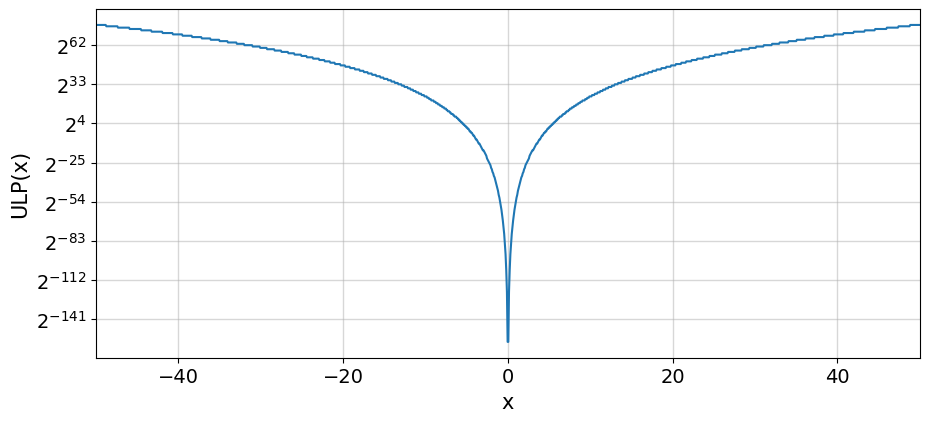
\includegraphics[width=.9\textwidth]{Imagens/ulps/ulp2}
  \caption{Função $ulp(x^{23})$ num sistema IEEE 754 de precisão dupla.}
  \label{fig:func_ulp}
\end{figure}

\subsection{Imprecisão de operações em Sistemas de Ponto flutuante}
Considere o cálculo de $f(x) = x^{10} + 1 - x^{10}$ para \(x \in [-60, 60]\).
As partes envolvendo $x$ são variáveis e a parte ``$1$'' é o literal, ou seja,
um valor fixo. Embora para $x \in \mathbb{R}$ o resultado de $f(x)$ seja igual
a 1, ao efetuarmos os cálculos usando ponto flutuante, observamos um
comportamento inesperado em que o valor correto é exibido apenas até um certo
valor de $x$. Após esse valor observamos um intervalo em que ocorre uma
oscilação no resultado da função e, em seguida, observamos que a função assume
o valor zero, como ilustrado na Figura~\ref{fig:catastrofic_cancelation}
e~\ref{fig:zoom}.

\begin{figure}[h]
  \centering
  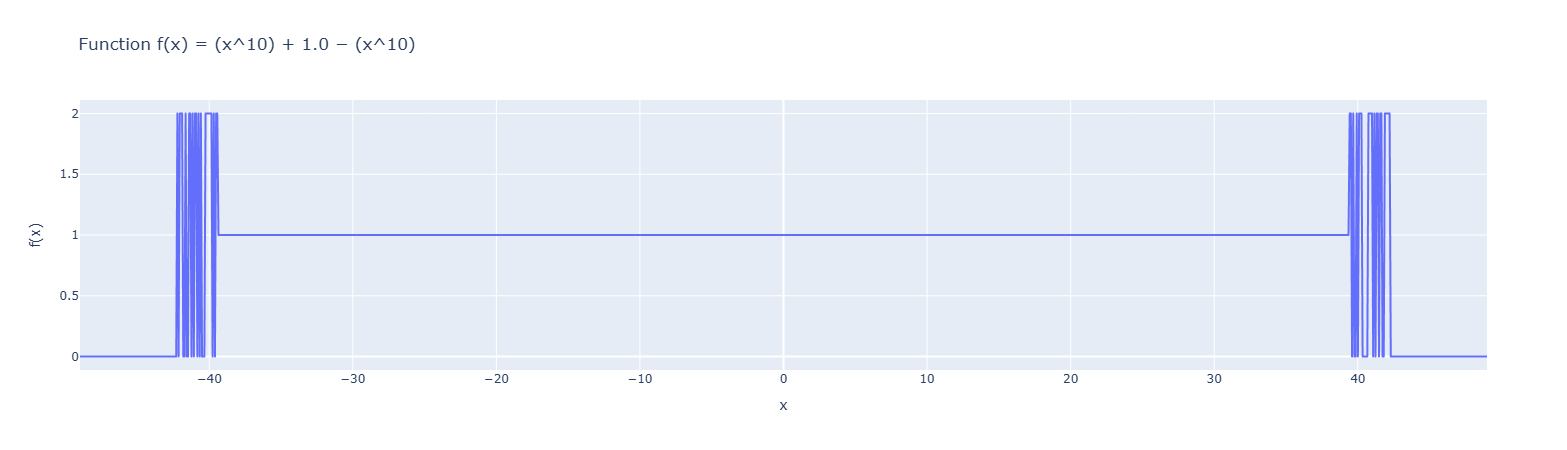
\includegraphics[width=1\textwidth]{Imagens/casosPeculiaresFP/catastrofic_cancelation.png}
  \caption{Comportamento da expressão \(x^{10} + 1 - x^{10}\) no intervalo \([-40, 40]\).}
  \label{fig:catastrofic_cancelation}
\end{figure}
\begin{figure}[h]
  \centering
  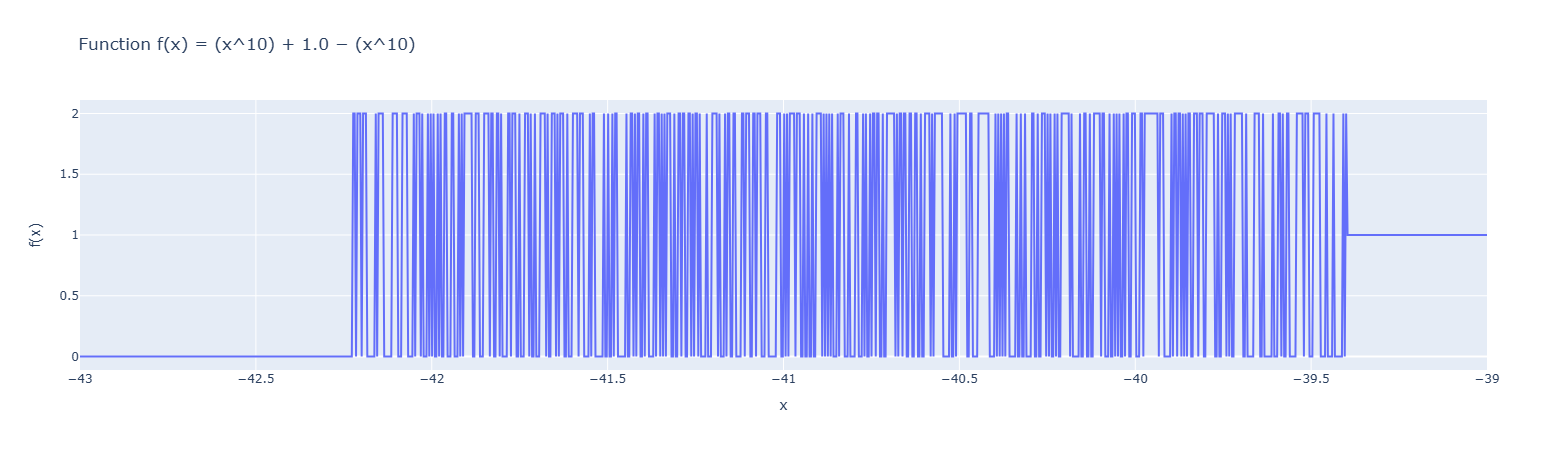
\includegraphics[width=1\textwidth]{Imagens/casosPeculiaresFP/zoom.png}
  \caption{Comportamento da expressão \(x^{10} + 1 - x^{10}\) no intervalo \([-43, -39]\).}
  \label{fig:zoom}
\end{figure}

A partir de um determinado limiar, a função para de se comportar como esperado
$f(x) = 1$ e passa a assumir valores os de $f(x) = 2$ e $f(x) = 0$. Vamos
manipular essa expressão e ver como ela se comporta em diferentes situações.

\begin{figure}[h]
  \centering
  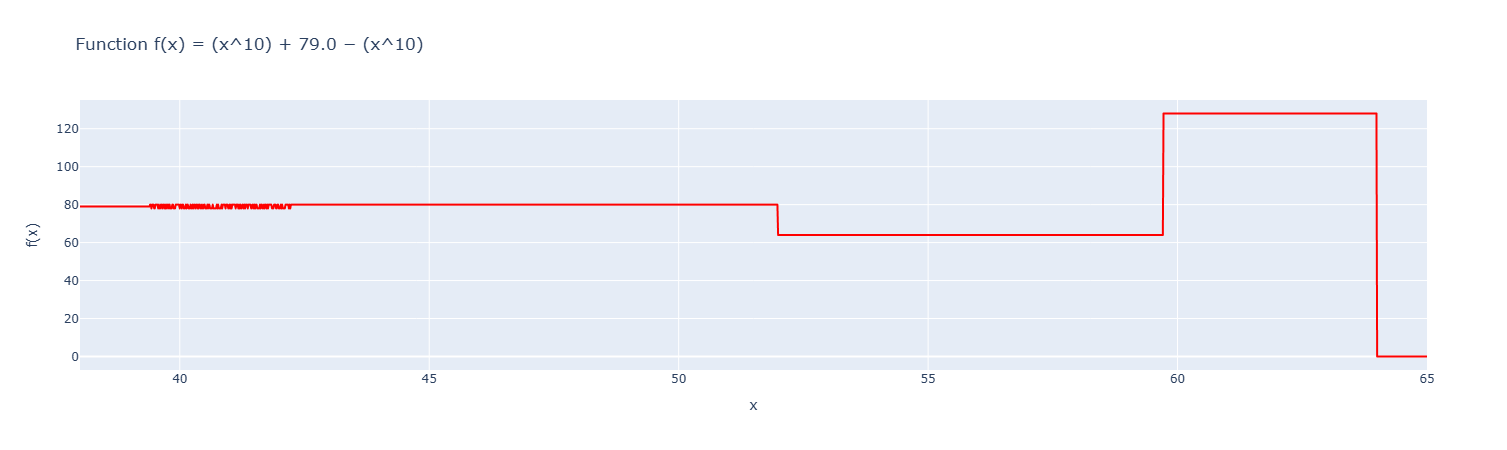
\includegraphics[width=1\textwidth]{Imagens/casosPeculiaresFP/literal79.png}
  \caption{Comportamento da expressão \(x^{10} + 79 - x^{10}\) no intervalo \([38, 65]\).}
  \label{fig:literal79}
\end{figure}

Na figura \ref{fig:literal79}. é possível observar que a função assume mais de
dois valores inesperados para $f(x)$, nesse caso, o conjunto imagem no
intervalo \([38, 65]\) é \( Im(f) = \bigl\{ {0{,}64{,}78{,}79{,}80{,}128}\}\).
O seguinte conjunto de valores para o literal foi testado \(\{3,12,79,98\}\), e
hipotetiza-se que para valores que não podem ser escritos como uma potência de
base 2, esse padrão ocorra.

Uma dúvida comum é se a precisão desses sistemas afeta nessa expressão. Vamos
comparar então um sistema de float32 (Cerca de 7-8 bits dígitos decimais de
precisão) a um sistema float64 (Cerca de 15-16 dígitos decimais de precisão)
\begin{figure}[h]
  \centering
  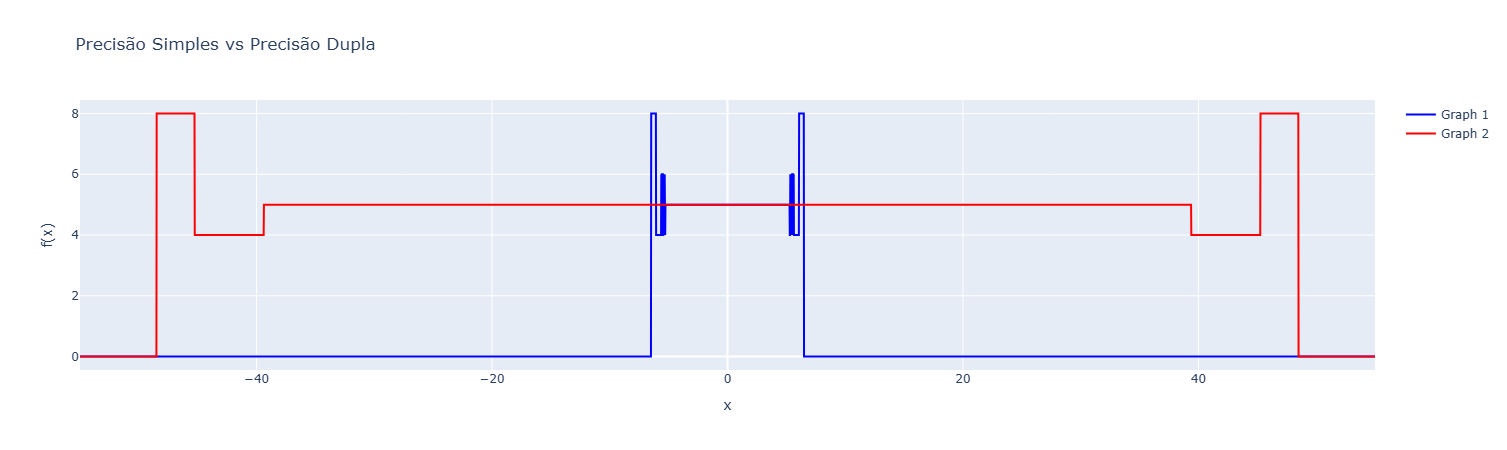
\includegraphics[width=1\textwidth]{Imagens/casosPeculiaresFP/32x64_full.png}
  \caption{Comportamento da expressão \(x^{10} + 2 - x^{10}\) no intervalo \([-40, 40]\).}
  \label{fig:32x64_full}
\end{figure}
\begin{figure}[H]
  \centering
  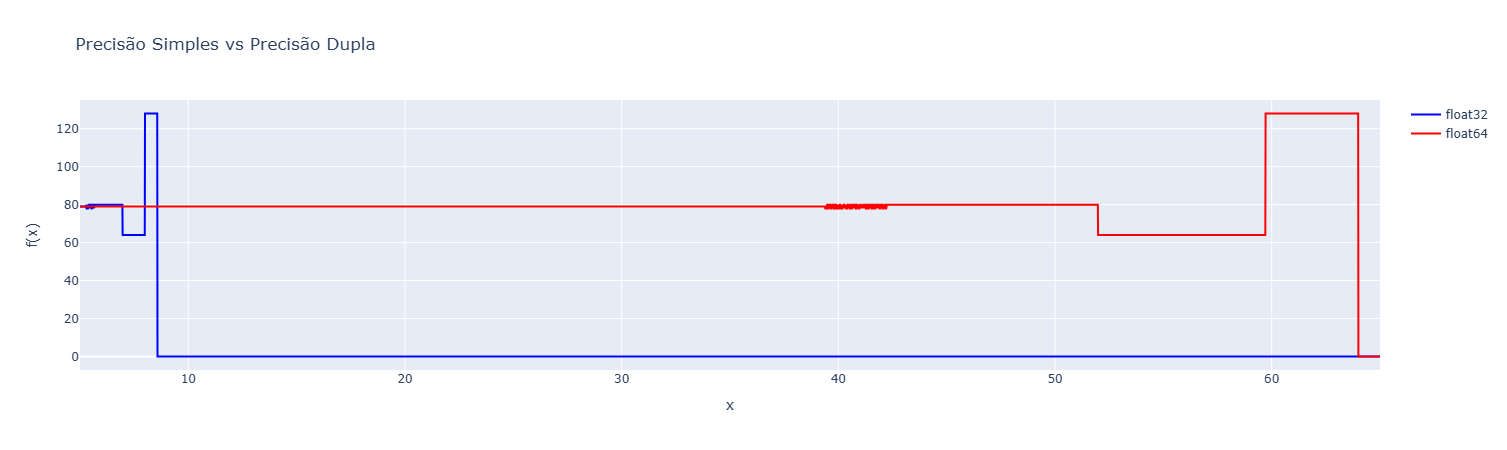
\includegraphics[width=1\textwidth]{Imagens/casosPeculiaresFP/32x64.png}
  \caption{Comportamento da expressão \(x^{10} + 79 - x^{10}\) no intervalo \([0, 60]\).}
  \label{fig:32x64}
\end{figure}
Dos testes experimentais, exemplificado nas figuras \ref{fig:32x64_full} e \ref{fig:32x64}, foi concluído que o $|x|$ onde a instabilidade ocorre é menor é menor na precisão dupla.

Outro caso interessante é quando analisamos a função $f(x) = (x\times x\times
  x\times x\times x\times x\times x\times x \times x) - x^{10} $. Vejamos o
gráfico dessa função.
\begin{figure}[H]
  \centering
  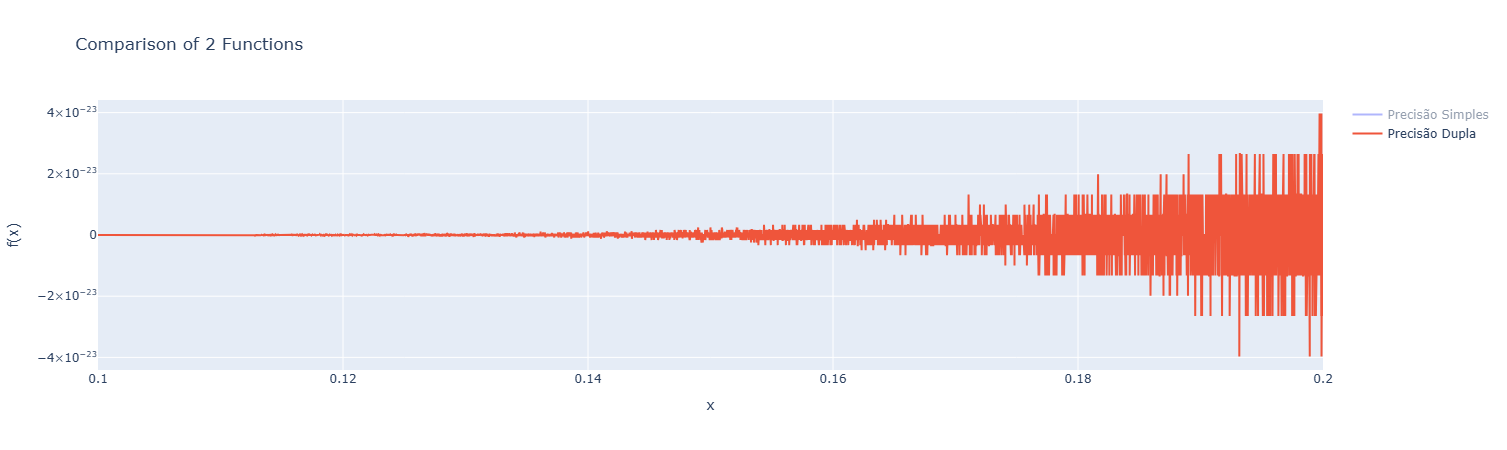
\includegraphics[width=1\textwidth]{Imagens/casosPeculiaresFP/timesXpot_literal0.png}
  \caption{Comportamento da expressão $f(x) = (x \times x \times x \times x \times x \times x \times x \times x \times x) - x^{10}$, com precisão dupla, no intervalo \([0{,}1, 0{,}2]\).}
  \label{fig:timesXpot_literal0}
\end{figure}
\begin{figure}[H]
  \centering
  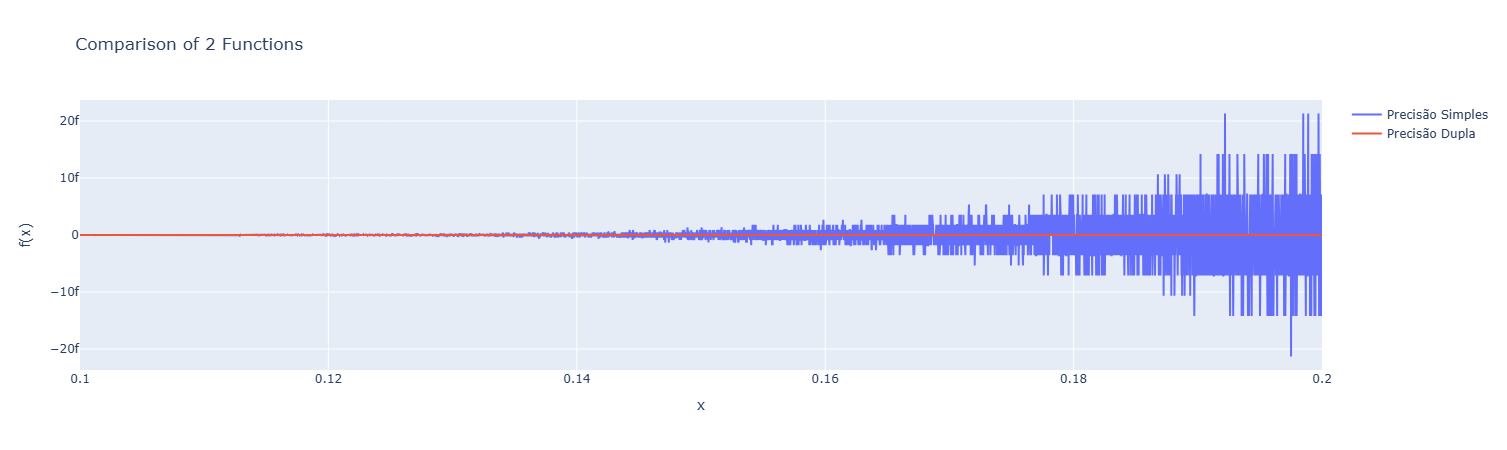
\includegraphics[width=1\textwidth]{Imagens/casosPeculiaresFP/timesXpot_literal0_1.png}
  \caption{Comportamento da expressão $f(x) = (x \times x \times x \times x \times x \times x \times x \times x \times x) - x^{10}$, com precisão simples, no intervalo \([0{,}1, 0{,}2]\).}
  \label{fig:timesXpot_literal0_1}
\end{figure}
A instabilidade na precisão dupla (Figura~\ref{fig:timesXpot_literal0_1}) produz imagem em torno de $[-4 \times 10^{-23},2 \times 10^{-23}]$, enquanto na precisão simples (Figura~\ref{fig:timesXpot_literal0}) está em torno de $[-20^{-15},20^{-15}]$ ($[-20 femto, 20 femto]$). Observa-se, portanto, que a diferença de instabilidade é extremamente menor na precisão dupla em comparação com a simples.

Uma outra situação é a diferença de como o computador interpreta algumas
funções se forem reescritas de maneiras diferentes. Seja $p(x) = (x - 1)^6$ e
$q(x) = x^6 - 6x^5 + 15x^4 - 20x^3 + 15x^2 - 6x + 1$, analiticamente essas
funções são idênticas, porém existem problemas de cancelamento catastrófico na
hora de analisarmos ambas em um sistema de ponto flutuante.

\begin{figure}[H]
  \centering
  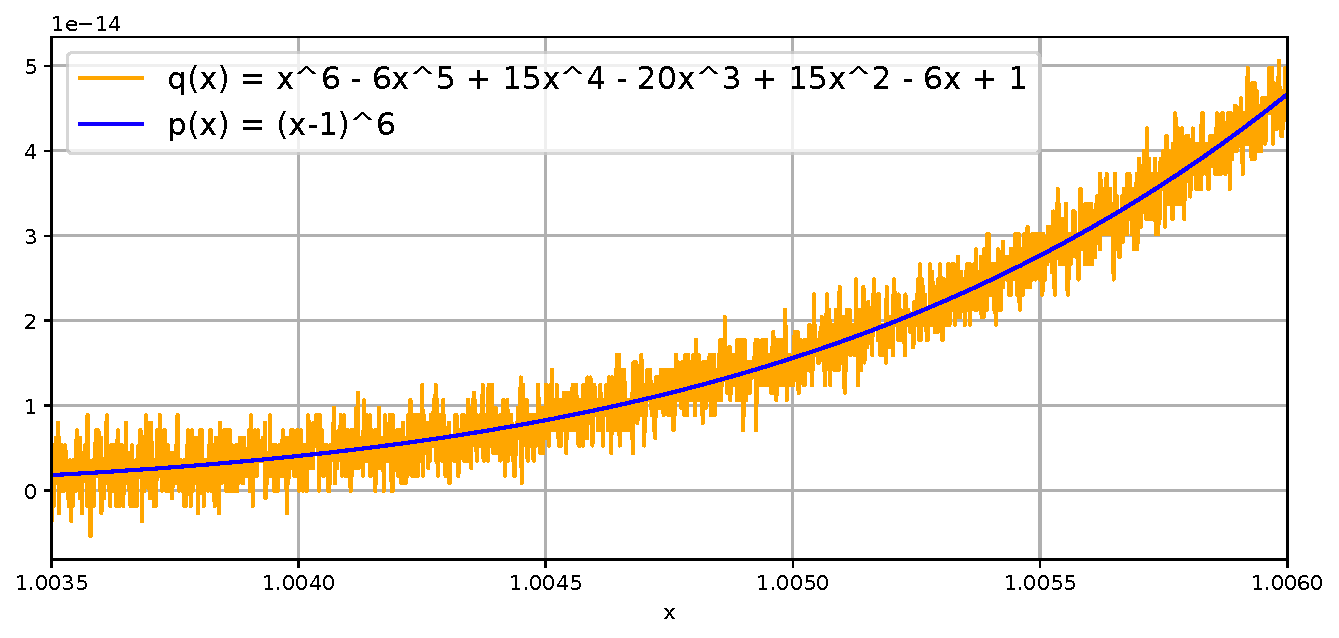
\includegraphics[width=1\textwidth]{Imagens/casosPeculiaresFP/NumError2_mplt}
  \caption{Comparação entre as funções $p(x) = (x - 1)^6$ e $q(x) = x^6 - 6x^5 + 15x^4 - 20x^3 + 15x^2 - 6x + 1$.}
  \label{fig:error2}
\end{figure}

\subsection{Discussão}

Esses exemplos destacam a importância da ordem das operações e da análise
cuidadosa ao trabalhar com algoritmos numéricos. Técnicas como a reordenação de
cálculos e o uso de formatos de precisão estendida podem ajudar a minimizar
esses erros em contextos críticos. Apesar de possivelmente surpreendentes,
esses fenômenos não invalidam a utilidade do ponto flutuante, pois o erro
observado tem ordem de grandeza muito pequena para a maioria das aplicações.

\chapter{Métodos Iterativos para Zeros de Função}

Em muitas aplicações, as soluções buscadas se resumem a encontrar os zeros (ou
raízes) de uma função. Entretanto, nem sempre é possível fazê-lo
analiticamente, devido à natureza das componentes envolvidas na função como,
por exemplo, funções polinomiais a partir do 3º grau, somas de funções
trigonométricas e logarítmicas, entre outras. Nesse ínterim, recorremos então a
maneiras de obter valores aproximados para tais raízes.

Uma classe de métodos utilizados para aproximar raízes de funções são os
\textbf{métodos iterativos}. A essência desses métodos está em, partindo de um
chute inicial e de uma função apropriada $\varphi$, obter uma sequência $x_k$
onde cada termo é obtido do anterior recursivamente como $x_{k+1} =
    \varphi(x_k)$. Essa sequência, sob certas hipóteses, converge para a raiz $\xi$
da função.

Ao longo do capítulo, reservaremos o símbolo $\xi$ para representar raízes de
funções.

\section{Localização de Raízes}

%Mais adiante no capítulo 
Nos métodos que trataremos nesse capítulo, para garantir a convergência da
sequência iterativa, é necessário que o primeiro termo esteja suficientemente
próximo da raiz e, desse modo, faz-se necessário restringir as funções a
intervalos que contenham raízes. Quando as funções envolvidas são contínuas, o
resultado a seguir garante a existência de raízes em um intervalo [a,b] desde
que as imagens dos extremos tenham sinais opostos.

\begin{prop}\label{c_tvi}%[Corolário do Teorema do Valor Intermediário]
    Seja $f(x)$ uma função contínua no intervalo $[a, b]$. Se $f(a)f(b) < 0$, então há pelo menos uma raiz $\xi \in (a,b)$. Se, além disso, existir $f'(x)$ e $f'(x)$ preservar o sinal em $(a,b)$, então a raiz é única.
\end{prop} %para todo d entre f(a) e f(b) existe ao menos um f(c) = d %então para f(a) > 0 e f(b) < 0, existe pelo menos um f(c) = 0
Por exemplo, considere a função $f(x) = x^3 - 9x + 3$. Utilizando a Proposição~\ref{c_tvi}, observamos que
\begin{itemize}
    \item $f(0)f(1) = -15 < 0$, portanto há raiz no intervalo (0, 1);
    \item $f(2)f(3) = -21 < 0$, portanto há raiz no intervalo (2, 3).
\end{itemize}
Além disso, a derivada de $f(x)$ é $f'(x) = 3x^2 - 9$, cujas raízes são $\pm \sqrt{3}$, então nos intervalos (-$\infty$, -$\sqrt{3}$), (-$\sqrt{3}$, $\sqrt{3}$) e ($\sqrt{3}$, $\infty$) o sinal da derivada é preservado. Portanto, nos intervalos $(0, 1)$ e $(2, 3)$ há apenas uma raiz.

\begin{figure}[h]
    \centering
    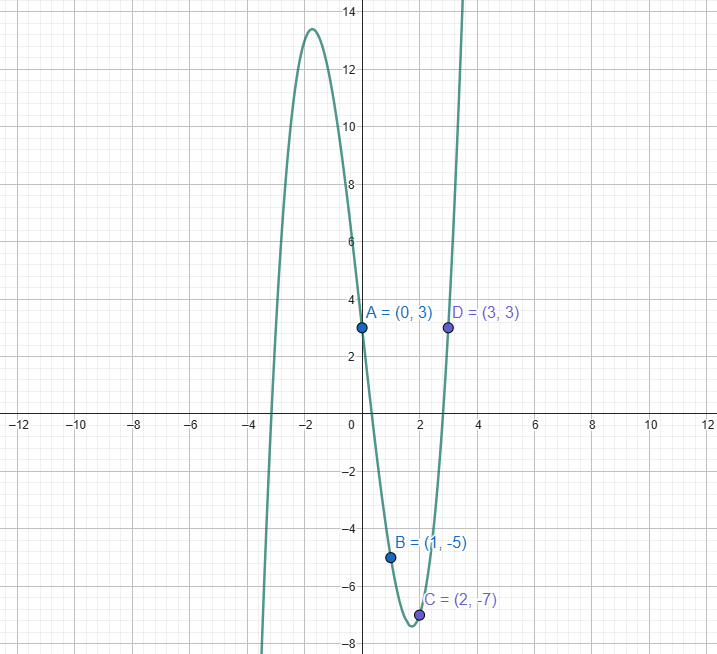
\includegraphics[height = 0.5\textwidth]{Imagens/fixedPoint/corolárioValorIntermed.png}
    \caption{Raiz entre A e B, e entre C e D}
    \label{fig:coro}
\end{figure}

\newpage

Outra forma de localizar raízes de uma dada função $f(x)$ é escrevê-la como a
diferença entre as funções $g(x)-h(x)$, pois se $f(\xi) = 0$ temos que $g(\xi)
    - h(\xi) = 0$ ou, equivalentemente, $g(\xi) = h(\xi)$. Graficamente, $\xi$ é a
abscissa do ponto de interseção entre as funções g(x) e h(x).

Da mesma função, podemos obter, por exemplo, as interseções entre $x$ e $x^3 -
    8x + 3$
\begin{figure}[h]
    \centering
    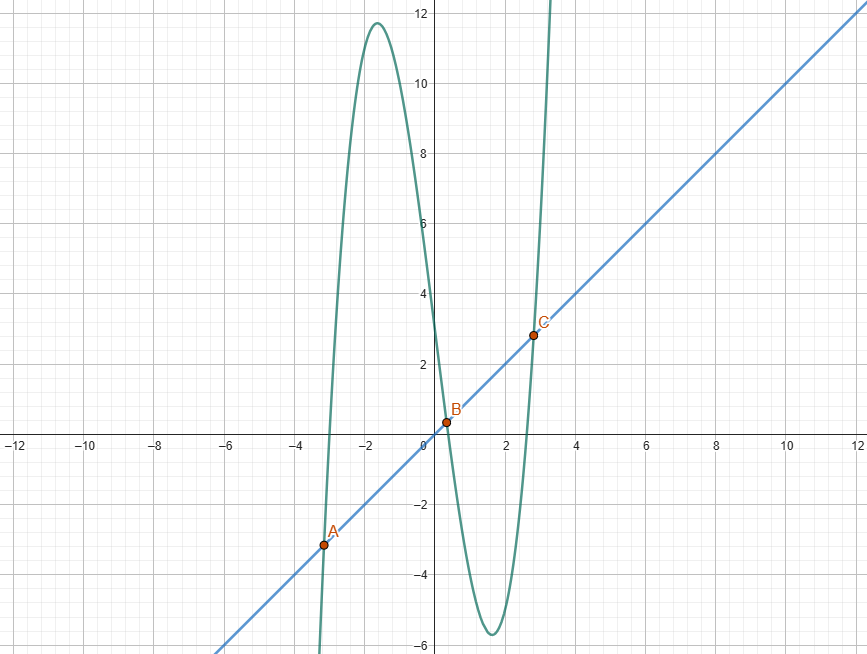
\includegraphics[height = 0.5\textwidth]{Imagens/fixedPoint/interseções.png}
    \caption{Interseções entre x e $x^3 - 8x + 3$}
    \label{fig:inters}
\end{figure}

\section{Critério de Parada}
\FIXME{Completar}
\DanielP{gráficos estilo Vera}
O processo é repetido até que a diferença entre duas iterações consecutivas seja inferior a uma tolerância pré-estabelecida %seja vertical (entre o valor da função e o eixo x) ou horizontal (entre o valor da sequência e $\xi$).
ou até que um número máximo de iterações seja atingido.

\begin{itemize} %era pra ficar topificado mesmo?
    \item $|\overline{x} - \xi| < \epsilon$ %x_{k+1} - x_k
    \item $f(\overline{x}) < \epsilon$
\end{itemize}

\LucasM{Definir raiz aproximada}

\section{Método do Ponto Fixo}

O método do ponto fixo \emph{é um método iterativo} que transforma o problema
de buscar as raízes de uma função $f(x)$ no problema de encontrar os pontos
fixos de uma outra função $\varphi(x)$, denominada de \textbf{função de
    iteração de ponto fixo}. A partir dessa função de iteração, uma sequência é
construída recursivamente começando em um valor inicial $x_0$ que convergirá
para a raiz $\xi$ de $f(x)$, desde que sejam observadas certas condições sob a
função $\varphi(x)$ e o dado inicial $x_0$.%parte da ideia de que as interseções de duas curvas construídas a partir de uma função f(x) revelam suas raízes para então construir uma função $\varphi(x)$ e buscar suas interseções com a reta identidade, que 

%Após localizar um intervalo que contenha uma raiz pelos métodos expostos,
O primeiro passo é gerar funções de iteração $\varphi$ para $f(x)$, o que pode
ser feito isolando $x$ na equação $f(x) = 0$. Por exemplo, manipulando a função
$x^3 -9x + 3$ da seguinte forma
\begin{equation*}
    x^3 - 8x + 3 = x
\end{equation*}
obtemos a função de iteração $\varphi(x) = x^3 - 8x + 3$. Com a mesma lógica, outras possíveis funções de iteração para $f$ são

\begin{multicols}{2}
    \begin{itemize} %itemize (era enumerate)
        \item[a)] $\varphi_1(x) = \frac{x^3}{9} + \frac{1}{3}$
        \item[b)] $\varphi_2(x) = \sqrt[3]{9x-3}$
        \item[c)] $\varphi_3(x) = \frac{9}{x} - \frac{3}{x^2}$
        \item[d)] $\varphi_4(x) = \sqrt{9 - \frac{3}{x}}$
        \item[e)] $\varphi_5(x) = -\sqrt{9 - \frac{3}{x}}$
        \item[f)] $\varphi_6(x) = x^3 - 8x + 3$
    \end{itemize}
\end{multicols}
A forma geral da função de iteração é
\begin{equation}
    \varphi(x) = x + A(x)f(x) \label{it}
\end{equation}
com $A(\xi) \ne 0$.
%É necessário verificar então se as funções de iteração geradas respeitam essa condição de $A(\xi) \neq 0$. 
Por exemplo, a $\varphi_1(x) = \frac{x^3}{9} + \frac{1}{3}$ na forma geral
ficaria
\begin{equation*}
    \varphi_1(x) = x + \frac{1}{9}f(x)
\end{equation*}
\begin{comment}
\varphi_1(x) &= x + \frac{1}{9}(x^3 - 9x + 3) \\
\varphi_1(x) &= x + \frac{x^3}{9} - x + \frac{1}{3} \\
\varphi_1(x) &= \frac{x^3}{9} + \frac{1}{3}
\end{comment}
em que $A(x) = \frac{1}{9}$. Nesse caso, pode-se observar que A($\xi) \neq 0$.

O resultado a seguir relaciona a raiz de uma função com pontos fixos de uma
função de iteração associada a essa função.

\begin{prop}
    Seja $\xi$ uma raiz de uma função $f(x)$ e seja $\varphi(x)$ uma função de iteração associada a $f(x)$. Então, $f(\xi) = 0$ se, e somente se, $\varphi(\xi) = \xi$.
\end{prop}

%Provando primeiramente que a raiz da função é ponto fixo da função de iteração, $f(\xi) = 0 \Rightarrow \varphi(\xi) = \xi$. Começa-se calculando a função de iteração para a raiz $\xi$, isto é, $\varphi(\xi)$, obtendo então, pela forma geral, a raiz somada ao produto da função A pela função original $ \xi + A(\xi)f(\xi)$. Dado que $\xi$ é raiz de f(x), o valor da função calculado em $\xi$ é 0, portanto se tem $\xi + A(\xi) \cdot 0$; o que anula o produto com a função A, $\xi + 0$. Com isso, concluí-se que a função de iteração calculada na raíz é de fato igual a $\xi$.

\begin{proof}
    ($\Rightarrow$) Pela forma geral da função de iteração temos que $\varphi(\xi) = \xi + A(\xi)f(\xi)$. Uma vez que $f(\xi) = 0$, então $\varphi(\xi) = \xi$.

    ($\Leftarrow$) Começando novamente pela forma geral da função de iteração, temos que $\varphi(\xi) = \xi + A(\xi)f(\xi)$. Como $\varphi(\xi) = \xi$, concluímos que $A(\xi) f(\xi) = 0$. Tendo como hipótese que $A(\xi) \neq 0$, então $f(\xi) = 0$.
    %ou seja, o ponto fixo $\xi$ da função de iteração $\varphi$ é raíz da função original $f(x)$. %q.e.d. (\textit{quod erat demonstrandum}, qual estava-se a demonstrar).
\end{proof}

%\newpage

\LucasM{Aqui, antes de ir para o resultado principal, dar exemplos de funções de iteração que fazem a sequencia convergir e divergir. Inserir gráficos assim como no livro da Vera.}
\DanielP{ok! uma redemoinho ($\varphi_6$: [$-\sqrt{3}$, $-\sqrt{\frac{7}{3}}$]), uma escadinha($\varphi_1$: [0, $\sqrt{3}$]) e uma divergente($\varphi_4$ e $\varphi_5$; $\varphi_2$ e $\varphi_3$ I)}

Sob condições a respeito da função de iteração, sua derivada e o dado inicial,
a convergência da sequência iterativa é garantida, como pode-se observar a
seguir.
%Enfim é importante verificar se a função de iteração de ponto fixo respeita as condições para convergência.
\begin{teo} \textbf{Convergência da Sequência Iterativa} \label{teoMPF}\\
    Seja $\xi$ uma raiz de f(x), isolada num intervalo I centrado nessa raiz. Considere uma função de iteração $\varphi(x)$ associada a f(x). Sob as seguintes hipóteses:
    \begin{itemize}
        \item[i)] $\varphi(x)$ e $\varphi'(x)$ são contínuas em I,
        \item [ii)] $|\varphi'(x)| \leq M < 1$ em I,
        \item [iii)] $x_0 \in I$,
    \end{itemize}
    a sequência $x_{k+1} = \varphi(x_k)$ converge para a raiz $\xi$.
\end{teo}
%Dada uma função $\varphi(x)$ ela é chamada de função de iteração, pois $\varphi(x_k) = x_{k+1}$ e através dessas iterações podemos buscar o ponto fixo dela na qual $x_k = \xi$. Provaremos a seguir que dada uma raíz $\xi$ de f(x) isolada num intervalo I centrado na mesma, a sequência recursiva $\varphi(x_k) = x_{k+1}$ converge para $\xi$ tendo: a função contínua e derivável, e sua derivada também contínua, no intervalo (a,b); o módulo (M) de sua derivada limitado e inferior a unidade no intervalo ($|\varphi'(x)| \leq M < 1$ $\forall x \in (a, b)$); e o primeiro valor da iteração no intervalo ($x_0 \in I$).
\begin{proof}
    Como $x_{k+1} = \varphi(x_k)$, subtraindo $\xi$ de ambos os lados da igualdade e usando o fato de que $\varphi(\xi)=\xi$ temos
    \begin{equation}\label{difIt}
        x_{k+1} - \xi = \varphi(x_k) - \varphi(\xi).
    \end{equation}
    Pelo Teorema do Valor Médio (TVM) podemos escrever \\
    \begin{equation}\label{tvm}
        \varphi(x_k) - \varphi(\xi) = \varphi'(c_k) (x_k - \xi)
    \end{equation}
    com $c_k$ entre $x_k$ e $\xi$. Então, substituindo (\ref{tvm}) em (\ref{difIt}), temos
    \begin{align}\label{des}
        %x_{k+1} - \xi &= (x_k - \xi) \ \varphi'(c_k) \\
        |x_{k+1} - \xi| & = |(x_k - \xi) \ \varphi'(c_k)| \nonumber \\
                        & = |x_k - \xi| \ |\varphi'(c_k)|           \\
                        & < |x_k - \xi| \nonumber
    \end{align}
    uma vez que $|\varphi'(x)| < 1$. Como $x_0 \in I$, podemos concluir que $x_k \in I$ para todo $k$ já que, por (\ref{des}), $|x_k - \xi| < |x_0 - \xi|$.

    Na sequência, provaremos que $x_k$ converge para a raiz $\xi$. Vamos começar
    mostrando que
    \begin{equation}\label{lab2}
        |x_1 - \xi| \leq M \ |x_0 - \xi|.
    \end{equation}
    Observe que, como $x_1=\varphi(x_0)$, temos que $x_1 - \xi = \varphi(x_0) - \varphi(\xi)$. Pelo Teorema do Valor Médio temos que $\varphi(x_0) - \varphi(\xi) = (x_0 - \xi) \ \varphi'(c_0)$, para algum $c_0$ entre $x_0$ e $\xi$. Uma vez que $|\varphi'(x)| \leq M$ no intervalo $I$, a seguinte desigualdade é válida
    \begin{align*}
        |x_1 - \xi| & = |x_0 - \xi| \ |\varphi'(c_0)| \\
                    & \leq M \ |x_0 - \xi|
    \end{align*}
    e provamos a desigualdade (\ref{lab2}).
    %\begin{align*}
    %    |x_1 - \xi| &= |\varphi(x_0) - \xi| \\
    %    \text{Pelo TVM,} \ \varphi(x_0) - \xi &= (x_0 - \xi) \ \varphi'(c_0) \text{, com $c_0 \in (x_0, \xi)$} \\
    %    |x_1 - \xi| &= |x_0 - \xi| \ |\varphi'(c_0)| \\
    %    \text{Como $|\varphi'(x)| \leq M$,} \ |\varphi'(c_0)| \ |x_0 - \xi| &\leq M \ |x_0 - \xi| \\
    %    |x_1 - \xi| &\leq M \ |x_0 - \xi|
    %\end{align*}
    De modo similar prova-se que $|x_2 - \xi| \leq M \ |x_1 - \xi|$ que, combinado
    com (\ref{lab2}), implica que $|x_2 - \xi| \leq M^2 \ |x_0 - \xi|$. Repetindo o
    processo k vezes pode-se concluir que
    \begin{equation}\label{lim0}
        |x_k - \xi| \leq M^k \ |x_0 - \xi|.
    \end{equation}
    Como $0 < M < 1$, se k tende a infinito, $M^k$ tende a 0 e, portanto, $M^k \ |x_0 - \xi|$ também tende a 0. Assim, provamos que
    %\begin{align*}
    %\lim_{k \to \infty} |x_k - \xi| &\leq M^k \ |x_0 - \xi| \\
    %\lim_{k \to \infty} |x_k - \xi| &\leq 0 \ |x_0 - \xi| \\
    %\lim_{k \to \infty} |x_k - \xi| &= 0 \ \text{logo, }
    %\end{align*}
    \begin{equation}
        \lim_{k \to \infty} x_k = \xi, \label{conv.mpf}
    \end{equation}
    ou seja, $x_k$ converge para a raiz.
\end{proof}

% $\varphi'(x) = \frac{x^2}{3}$ \\ $|\varphi'(x)| < 1$ para $x \in (-\sqrt{3}, \sqrt{3})$ 

\subsection{Ordem de convergência}

A ordem de convergência de um método iterativo é uma medida de quão rapidamente
a sequência de iterações converge para a solução desejada. Em termos práticos,
isso significa que, se um método tem uma ordem de convergência alta, ele será
capaz de reduzir mais o erro de aproximação a cada iteração.
\begin{df}
    Seja $\{x_k\}$ uma sequência que converge para $\xi$ e
    \begin{equation} \label{erro}
        e_k = x_k - \xi
    \end{equation}
    o erro na k-ésima iteração.
    %um num. p e uma cte. C
    Se existirem $p > 1$ e $C > 0$ tais que $\lim_{k \to \infty}
        \frac{|e_{k+1}|}{|e_k|^p} = C$, então $p$ é chamada de \emph{ordem de
        convergência} da sequência e $C$ é a \emph{constante assintótica de erro}.
\end{df}

\begin{comment} sobre p
A ordem de convergência $p$ de um método iterativo fornece uma informação sobre a rapidez de convergência do processo, pois podemos reescrever (\ref{conv}) como $|e_{k+1}| = C |e_k|^p$ para k tendendo ao infinito.

Uma vez que a sequência {$x_k$} é convergente, $e_k$ tende a 0 quando $k$ tende
ao infinito, portanto, quanto maior for $p$ mais próximo de 0 estará $C|e_k|^p$
(independente de C), implicando numa convergência mais rápida da sequência.
Assim, se dois processos iterativos resultam em sequências {$x_k^1$} e
    {$x_k^2$}, ambas convergindo para $\xi$, com suas respectivas ordens de
convergência $p_1$ e $p_2$, se $p_1 > p_2 \geq 1$, o processo que gera a
sequência {$x_k^1$} converge mais rapidamente.
\end{comment}
%$|e_{k+1}| \approx C |e_k|^p$
No caso do MPF verificaremos que $p = 1$ portanto a ordem de convergência do
método é ao menos linear.
\begin{prop}
    Se
    \begin{equation}\label{conv}
        \lim_{k \to \infty} \frac{e_{k+1}}{e_k} = C, \ 0 \leq |C| < 1,
    \end{equation}
    então a convergência é pelo menos linear. O MPF tem convergência pelo menos linear.
\end{prop}
\begin{proof}
    Partindo de (\ref{difIt}) e (\ref{tvm}), e tomando o  limite com k tendendo a infinito, podemos escrever (\ref{conv}) como
    \begin{equation*} %\frac{x_{k+1} - \xi}{x_k - \xi} = \varphi'(c_k)
        \lim_{k \to \infty} \frac{x_{k+1} - \xi}{x_k - \xi} = \lim_{k \to \infty}\varphi'(c_k)
    \end{equation*} %se $x_k$ converge para $\xi$ então $c_k$ também converge para $\xi$.
    com $c_k$ entre $x_k$ e $\xi$
    %, obtendo $C = \varphi'(\xi)$, pois, assim como $x_k$, $c_k$ converge para $\xi$
    . %análogo ao uso de (2.4) antes de (2.5), certo?
    %é necessário, mostrar que \varphi'(\lim_{k \to \infty} c_k) = \varphi'(\xi)? uma vez que o que importa é que \varphi'(x) < 1 independente do x
    Como por hipótese $|\varphi'(x)| < 1$ então $|C| < 1$, portanto, a convergência
    do MPF é pelo menos linear.
\end{proof}
\newpage

\subsection{Implementações do Método do Ponto Fixo}

\subsubsection{Imperativa}

\begin{algorithm}[H]
    \caption{Método do Ponto Fixo Iterativo}
    \label{alg:pontofixo_imperativo}
    \begin{algorithmic}[1]
        \Procedure{Main}{}
        \State $x_0 \gets 1.5$ \Comment{Chute inicial}
        \State $\text{tol} \gets 10^{-6}$ \Comment{Tolerância}
        \State $N \gets 100$ \Comment{Número máximo de iterações}

        \State Inicializar vetor $H$ de tamanho $N+1$ \Comment{Alocação dinâmica}
        \State $x \gets x_0$
        \State $H[0] \gets x_0$

        \For{$i \gets 0$ \textbf{to} $N$}
        \State $x_{\text{next}} \gets \sin(x^2 + \cos(x))$ \Comment{Função $g(x)$}
        \State $H[i+1] \gets x_{\text{next}}$ \Comment{Salva no histórico}

        \If{$|x_{\text{next}} - x| < \text{tol}$}
        \State \textbf{Imprimir} "Raiz: " $x_{\text{next}}$
        \State \textbf{Imprimir} "Iterações: " $i+1$
        \State \textbf{Imprimir} Histórico $H[0 \dots i+1]$
        \State \Return 0 \Comment{Sucesso}
        \EndIf

        \State $x \gets x_{\text{next}}$ \Comment{Atualiza para próxima iteração}
        \EndFor

        \State \textbf{Imprimir} "Falha na convergência"
        \State Liberar memória de $H$
        \State \Return 1
        \EndProcedure
    \end{algorithmic}
\end{algorithm}

\subsubsection{Funcional}

\begin{algorithm}[H]
    \caption{Método do Ponto Fixo Recursivo}
    \label{alg:pontofixo_funcional}
    \begin{algorithmic}[1]
        \Function{g}{$x$}
        \State \Return $\sin(x^2 + \cos(x))$
        \EndFunction

        \Procedure{FixedPoint}{$x_0, \text{tol}, \text{maxIters}$}

        \Function{Go}{$x, \text{iter}, \text{acc}$} \Comment{Função auxiliar recursiva}
        \If{$\text{iter} \geq \text{maxIters}$}
        \State \Return $(x, \text{iter}, \text{acc})$ \Comment{Limite atingido}
        \EndIf

        \State $x_{\text{next}} \gets g(x)$

        \If{$|x_{\text{next}} - x| < \text{tol}$}
        \State \Return $(x_{\text{next}}, \text{iter} + 1, \text{acc} \cup [x_{\text{next}}])$ \Comment{Convergiu}
        \Else
        \State \Return \Call{Go}{$x_{\text{next}}, \text{iter} + 1, \text{acc} \cup [x_{\text{next}}]$} \Comment{Recursão}
        \EndIf
        \EndFunction

        \State \Return \Call{Go}{$x_0, 0, [x_0]$} \Comment{Chamada inicial com lista [x0]}
        \EndProcedure
    \end{algorithmic}
\end{algorithm}

%--------------------------------------------------------------------
\section{Método de Newton-Raphson Unidimensional}\label{sec:NR1d}

\TODO{talvez reescrever todas as condições como i) derivada limitada ii) f e g continuas , etc...}

\DanielP{conv quadrática}

\EnzoR{escolhendo a func de iter}

O método de Newton é um caso particular do \textbf{Método do Ponto Fixo}
amplamente utilizado para encontrar raízes reais de funções não lineares, cuja
ordem de convergência é pelo menos quadrática. A função de iteração específica
para este método produz uma sequência em que cada termo $x_{k+1}$ corresponde,
geometricamente, à \textbf{interseção da reta tangente} a $f(x)$ no ponto
$(x_k, f(x_k))$ com o eixo x. %\EnzoR{seria raízes complexas, não?} 

\subsection{Sequência Iterativa}
\DanielP{Talvez mudar o nome}
No método do ponto fixo, vimos que se a função satisfaz o Teorema \ref{teoMPF} a sequência $x_{k+1} = \varphi(x_k)$ converge para $\xi$. Além disso, da desigualdade (\ref{lim0}) temos que quanto menor for $|\varphi'(x)|$, mais rápido a sequência $\{x_k\}$ converge.

Aplicando a derivada na forma geral de $\varphi$ pela regra da cadeia obtemos
$\varphi'(x) = 1 + A'(x)f(x) + A(x)f'(x)$ e, calculando-a na raiz, obtemos
$\varphi'(\xi) = 1 + A(\xi)f'(\xi)$. Usando $\varphi'(\xi) = 0$, concluímos que
$A(\xi) = \frac{-1}{f'(\xi)}$. Generalizando, temos $A(x) = \frac{-1}{f'(x)}$.
Portanto, desde que $f'(x) \neq 0$, a forma da função de iteração do método de
Newton-Raphson é
\begin{equation} \label{phiNR1d}
    \varphi(x) = x - \frac{f(x)}{f'(x)}.
\end{equation}

Dada uma função \(f(x)\), o processo parte de uma estimativa inicial \(x_0\) e
aplica a seguinte fórmula iterativa, a partir da escolha da derivada em
(\ref{it})
\begin{equation} \label{nr}
    x_{k+1} = x_k - \frac{f(x_k)}{f'(x_k)},
\end{equation}
onde \(f'(x_k)\) é a derivada da função \(f\) avaliada em \(x_k\).
Para que o método convirja para a raiz correta, é necessário que \(f(x)\) seja continuamente diferenciável em uma vizinhança da raiz e que \(f'(x) \neq 0\) nessa região. Além disso, a escolha adequada do ponto inicial \(x_0\) é crucial para garantir a convergência do método.

\subsection{Interpretação Geométrica}
\DanielP{ficou paia o alinhamento em}
\begin{align*}
    f'(x_0)(x - x_k)       & = y - y_k                   \\
    f'(x_k)(x_{k+1} - x_k) & = -y_k                      \\
    x_{k+1} - x_k          & = \frac{-y_k}{f'(x_k)}      \\
    x_{k+1}                & = x_k - \frac{y_k}{f'(x_k)}
\end{align*}
\subsection{Convergência}
O método de Newton-Raphson apresenta convergência local quadrática sob certas
condições. Isso significa que, se o ponto inicial $x_0$ estiver suficientemente
próximo da raiz simples $\xi$ e $f$, $f'$ e $f''$ forem contínuas em uma
vizinhança de $\xi$ com $f'(\xi) \neq 0$, então a sequência $\{x_k\}$ definida
por $x_{k+1} = x_k - \frac{f(x_k)}{f'(x_k)}$ converge para $\xi$ e o erro
$e_{k} = x_k - \xi$ satisfaz
\[
    |e_{k+1}| \leq C |e_k|^2
\]
para algum $C > 0$ e $k$ suficientemente grande. Assim, a cada iteração, o
número de dígitos corretos aproximadamente dobra, caracterizando convergência
quadrática.
\begin{teo} \label{teoNR}
    Sejam $f(x)$, $f'(x)$ e $f''(x)$ contínuas num intervalo $I$ que contém a raiz $\xi$ de $f$, supondo $f'(\xi) \neq 0$. Então, existe um intervalo $\overline{I} \subset I$, contendo a raiz $\xi$, tal que $x_0 \in \overline{I}$, a sequência ${x_k}$ gerada pela função de iteração $\varphi(x) = x - \frac{f(x_k)}{f'(x_k)}$ convergirá para a raiz.
\end{teo}
\begin{proof}
    Sendo o método de Newton-Raphson um caso particular do MPF, basta provar que para $\varphi(x) = x - \frac{f(x)}{f'(x)}$ as hipóteses do Teorema \ref{teoMPF} são satisfeitas.

    Primeiramente, observe que
    \begin{equation} \label{dphiNR}
        \varphi'(x) = \frac{f(x)f''(x)}{[f'(x)]^2}.
    \end{equation}
    Como $f'(\xi) \neq 0$ e $f'(x)$ é contínua em I, é possível obter $I_1 \subset I$ tal que $f'(x) \neq 0$ no intervalo $I_1$. Assim, a função $f$ e suas derivadas primeira e segunda são contínuas em $I_1$ e, consequentemente, a função de iteração e sua derivada também.

    Uma vez que a $\varphi'(x)$ é contínua em $I_1$ e $\varphi'(\xi) = 0$, é
    possível escolher $I_2 \subset I_1$ de modo que $|\varphi'(x)| < 1$ em $I_2$
    tendo $\xi$ como centro do novo intervalo.

    Por fim, tomando, $\overline{I} = I_2$, satisfazem-se as hipóteses do Teorema
    \ref{teoMPF}.
\end{proof}
\subsection{Ordem de Convergência}
No MPF espera-se uma ordem de convergência ao menos linear, entretanto ao
escolher uma função de iteração que satisfaça $\varphi'(\xi) = 0$, provaremos
que sua ordem de convergência será ao menos quadrática.
\begin{prop}
    A ordem de convergência do método de Newton é pelo menos quadrática.
\end{prop}
\begin{proof}
    Assumiremos todas as hipóteses do Teorema \ref{teoNR}. %(de Convergência do Método de Newton-Raphson), temos
    Partindo de $x_{k+1} = x_k - \frac{f(x_k)}{f'(x_k)}$, subtraindo $\xi$ em ambos os lados da igualdade, obtemos
    \begin{equation} \label{eMNR}
        e_{k+1} = e_k - \frac{f(x_k)}{f'(x_k)}
    \end{equation}
    O polinômio de Taylor de grau 2 para $f(x)$ centrado em $x_k$ é
    \begin{equation*}
        f(x) = f(x_k) + f'(x_k)(x - x_k) + \frac{f''(c_k)}{2}(x-x_k)^2
    \end{equation*}
    com $c_k$ entre $x$ e $x_k$.
    %$-(x-x_k)$
    Assim, $f(\xi) = f(x_k) - f'(x_k)(x_k - \xi) + \frac{f''(c_k)}{2}(x_k-\xi)^2$
    dado que $f(\xi) = 0$, dividindo a equação pela derivada de $f$ temos,
    aplicando a fórmula do erro \ref{erro} e a da sequência \ref{nr}
    \begin{align*}
        e_k - \frac{f(x_k)}{f'(x_k)} & = \frac{f''(c_k)}{2f'(x_k)}e_k^2       \\
        e_{k+1}                      & = \frac{f''(c_k)}{2f'(x_k)}e_k^2       \\
        \frac{e_{k+1}}{e_k^2}        & = \frac{1}{2} \frac{f''(c_k)}{f'(x_k)}
    \end{align*}

    Aplicando limite no termo esquerdo da equação acima e, dada a continuidade das
    funções, nos argumentos à direita, obtemos
    \begin{equation*}
        \lim_{k \to \infty} \frac{e_{k+1}}{e_k^2} = \frac{1}{2} \frac{f''(\xi)}{f'(\xi)}
    \end{equation*}
    \LucasM{Reescrever isto}
    \EnzoR{Como?}
    Calculando a $\varphi''$ a partir de $\varphi'$ \ref{dphiNR} %temos $\frac{[f'(x)f''(x)+f(x)f'''(x)][f'(x)]^2 - 2f'(x)f''(x)f(x)f''(x)}{[f'(x)]^4}$, 
    em $\xi$ obtemos $\frac{[f'(\xi)]^3f''(\xi)}{[f'(\xi)]^4}$, que é um $C$ concluindo então que a convergência do método de Newton Raphson é ao menos quadrática.
    \begin{align*}
        \lim_{k \to \infty} \frac{e_{k+1}}{e_k^2} & = \frac{1}{2} \varphi''(\xi) \\
                                                  & = C
    \end{align*}
    %\frac{f(x_k)}{f'(x_k)} &= e_k - \frac{f''(c_k)}{2f'(x_k)}e_k^2
\end{proof}

\subsection{Implementações do Método de Newton-Raphson Unidimensional}

\subsubsection{Imperativa}

\begin{algorithm}[H]
    \caption{Newton-Raphson Iterativo}
    \label{alg:newton_imperativo}
    \begin{algorithmic}[1]
        \Procedure{NewtonIter}{$f, f', x_0, \text{maxIter}$}
        \State $x \gets x_0$ \Comment{Inicialização da variável}
        \For{$i \gets 0$ \textbf{to} $\text{maxIter}$}
        \State $fx \gets f(x)$
        \State $dfx \gets f'(x)$
        \State $x_{\text{next}} \gets x - \frac{fx}{dfx}$
        \State $x \gets x_{\text{next}}$ \Comment{Atualiza o valor atual}
        \EndFor
        \State \Return $x$
        \EndProcedure
    \end{algorithmic}
\end{algorithm}

\subsubsection{Funcional}

\begin{algorithm}[H]
    \caption{Newton-Raphson Recursivo}
    \label{alg:newton_funcional}
    \begin{algorithmic}[1]
        \Procedure{NewtonRecursive}{$f, f', x_0, \text{maxIter}$}

        \Function{Iterate}{$x, n$} \Comment{Função auxiliar (cláusula where)}
        \If{$n = 0$}
        \State \Return $x$ \Comment{Caso base: fim das iterações}
        \Else
        \State $x_{\text{next}} \gets x - \frac{f(x)}{f'(x)}$
        \State \Return \Call{Iterate}{$x_{\text{next}}, n - 1$} \Comment{Passo recursivo}
        \EndIf
        \EndFunction

        \State \Return \Call{Iterate}{$x_0, \text{maxIter}$} \Comment{Chamada inicial}
        \EndProcedure
    \end{algorithmic}
\end{algorithm}

\subsection{Casos Atípicos}
O Método de Newton é amplamente utilizado na prática devido à sua rapidez e
precisão em condições ideais. Contudo, em algumas situações ele pode falhar ou
convergir para raízes incorretas se essas condições não forem satisfeitas.
Estes problemas geralmente estão associados a fatores como: pontos de máximo e
mínimo, pontos de inflexão, multiplicidade da raiz e escolha inadequada do
chute inicial.

\subsubsection{Caso 1: Alta multiplicidade de raízes}
Polinômios de grau elevado tendem a ter alta multiplicidade nas raízes, como no
caso do polinômio $x^{10} - 1$. A convergencia lenta é causada pela
multiplicidade da raiz. Quando uma raiz tem multiplicidade $m > 1$ — neste caso
$m = 10$ — a derivada próxima a raiz se aproxima de zero, aumentando o número
de iterações necessárias para convergir para a raiz. Isso faz com que a taxa de
convergência do metodo de Newton reduza-se para linear em vez da esperada taxa
quadrática.
\begin{figure}[H]
    \centering
    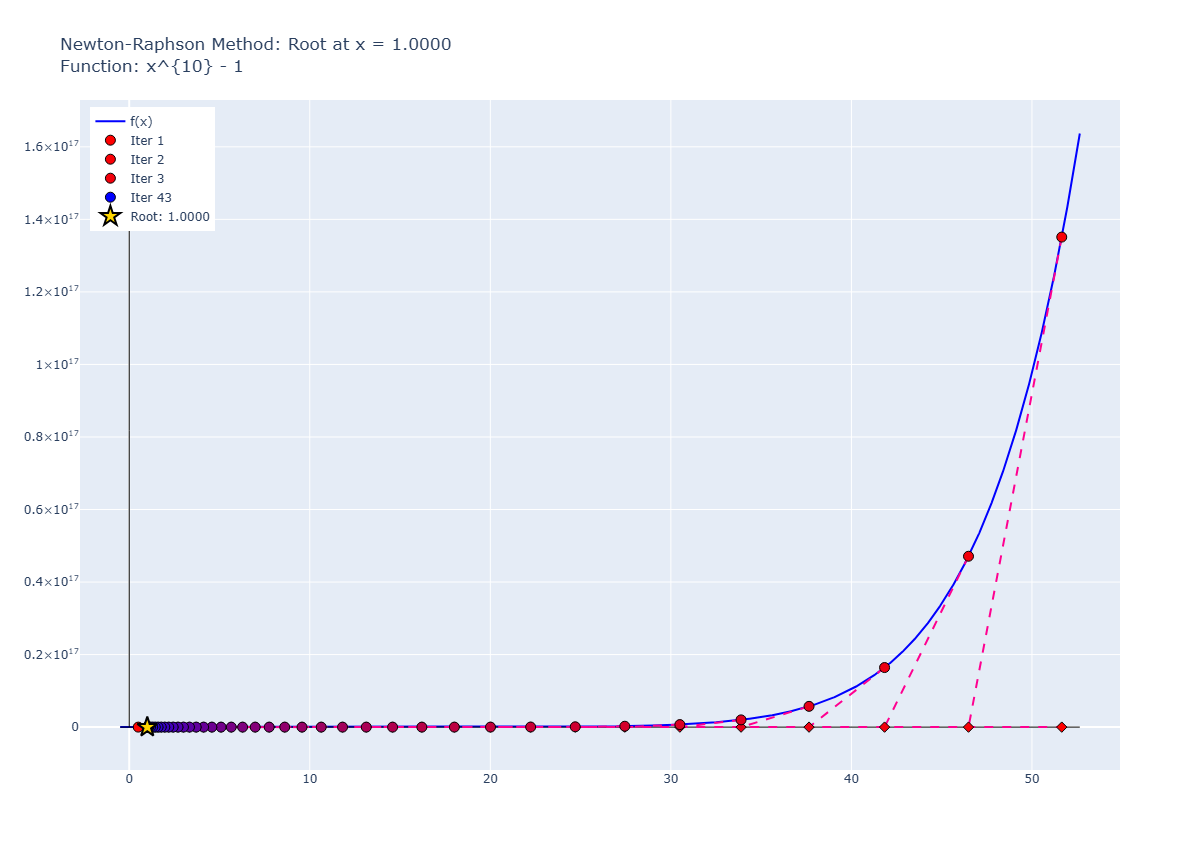
\includegraphics[width=1\textwidth]{Imagens/pitfalls/01/x_10-1.png}
    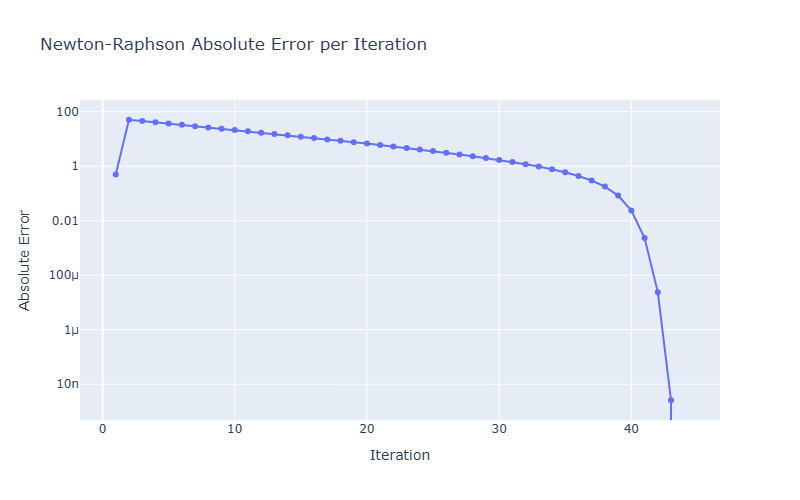
\includegraphics[width=1\textwidth]{Imagens/pitfalls/01/err_x_10-1.png}
    \caption{Gráfico daCilada relacionada a multiplicidade da raiz.}
    \label{fig:ciladaMultRaiz}
\end{figure}

Ao analisar a função geometricamente, é possível observar que a inclinação da
tangente à curva em torno da raiz é muito próxima de zero, o que resulta em
saltos minúsculos a cada iteração, causando uma convergencia lenta.

\begin{center}
    \small
    \begin{tabular}{|c|c|c|c|}
        \hline
        Iteração & Valor de $x_k$             & $f(x)$                        & Erro $e_k$             \\
        \hline
        1        & $x = 0.50000000000000000$  & $f(x) = -0.99902343750000000$ & $0.50000000000000000$  \\
        \hline
        2        & $x = 51.64999999999999858$ & $f(x) = 135114904483913696$   & $50.64999999999999858$ \\
        \hline
        3        & $x = 46.48499999999999943$ & $f(x) = 47111654129711536$    & $45.48499999999999943$ \\
        \hline
        4        & $x = 41.83650000000000091$ & $f(x) = 16426818072478544$    & $40.83650000000000091$ \\
        \hline
        5        & $x = 37.65285000000000082$ & $f(x) = 5727677301318307$     & $36.65285000000000082$ \\
        \hline
        $\vdots$ & $\vdots$                   & $\vdots$                      & $\vdots$               \\
        \hline
        43       & $x = 1.00000000257760013$  & $f(x) = 0.00000002577600156$  & $0.00000000257760013$  \\
        \hline
        44       & $x = 1.0$                  & $f(x) = 0.0$                  & $0.0$                  \\
        \hline
    \end{tabular}
    \label{tab:ciladaMultRaiz}
\end{center}

\subsubsection{Caso 2: Proximidade a extremos de função}
Outro fator que é um problema quando se trata de taxa de convergência são os
pontos de máximo e mínimo da função. Quando uma iteração é iniciada perto de um
ponto de máximo ou mínimo um dos problemas que podem ocorrer é a função de
iteração convergir para um ponto de máximo ou mínimo ao invés da raiz. Isso
pode causar uma diminuição na taxa de convergência.
\begin{figure}[H]
    \centering
    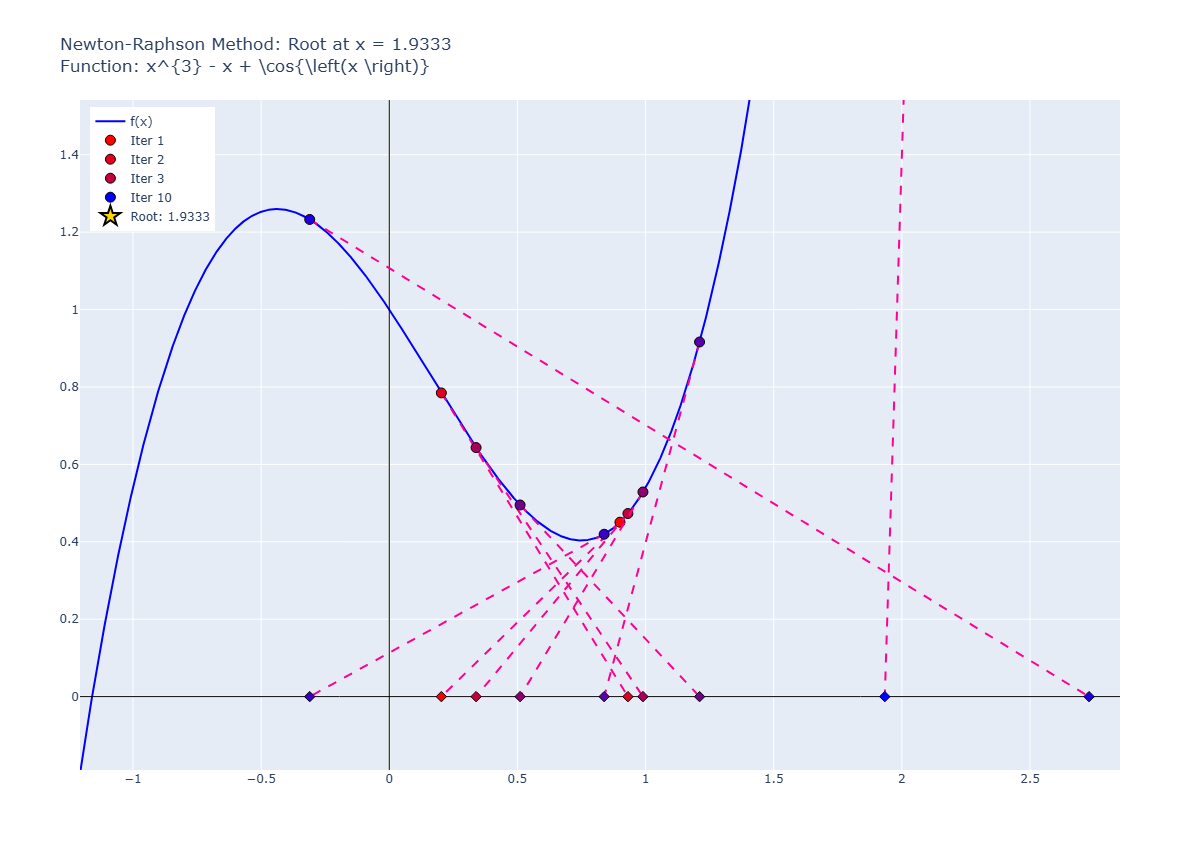
\includegraphics[width=1\textwidth]{Imagens/pitfalls/02/max_min.png}
    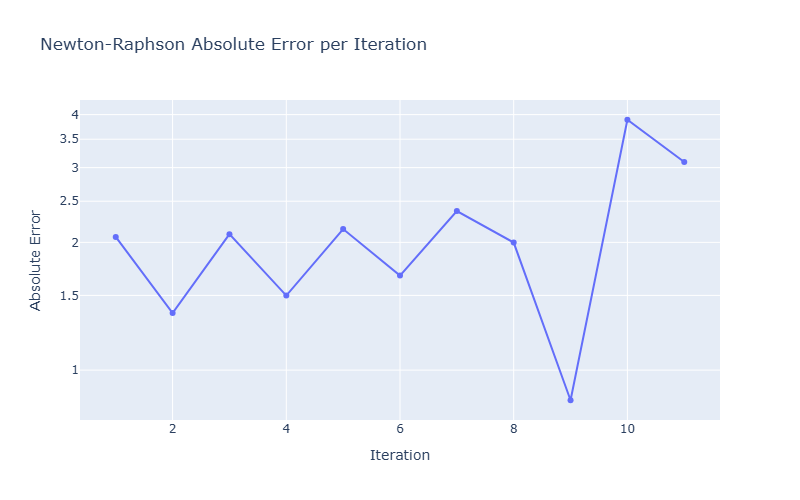
\includegraphics[width=1\textwidth]{Imagens/pitfalls/02/err_max_min.png}
    \caption{Cilada de ponto de Mínimo diminuindo a taxa de convergência.}
    \label{fig:ciladaMinMax_A}
\end{figure}

\begin{center}
    \small
    \begin{tabular}{|c|c|c|c|}
        \hline
        Iteração & Valor de $x_k$             & $f(x)$                        & Erro $e_k$            \\
        \hline
        1        & $x = 0.90000000000000002$  & $f(x) = 0.45060996827066446$  & $2.05960580450169983$ \\
        \hline
        2        & $x = 0.20318738327105890$  & $f(x) = 0.78462959591676906$  & $1.36279318777275882$ \\
        \hline
        3        & $x = 0.93108680836493152$  & $f(x) = 0.47305585213356149$  & $2.09069261286663144$ \\
        \hline
        4        & $x = 0.33865524784873213$  & $f(x) = 0.64338650465768399$  & $1.49826105235043205$ \\
        \hline
        5        & $x = 0.98975277280548202$  & $f(x) = 0.52871601875798535$  & $2.14935857730718194$ \\
        \hline
        6        & $x = 0.51038365868141022$  & $f(x) = 0.49512408543110442$  & $1.66998946318311026$ \\
        \hline
        7        & $x = 1.21066335888968579$  & $f(x) = 0.91621158441747408$  & $2.37026916339138571$ \\
        \hline
        8        & $x = 0.83841140043105933$  & $f(x) = 0.41958113044930967$  & $1.99801720493275914$ \\
        \hline
        9        & $x = -0.31043606990472872$ & $f(x) = 1.23271962647527022$  & $0.84916973459697120$ \\
        \hline
        10       & $x = 2.73020451984058488$  & $f(x) = 16.70421900417551697$ & $3.88981032434228480$ \\
        \hline
        11       & $x = 1.93332993606072678$  & $f(x) = 4.93835804267838796$  & $3.09293574056242671$ \\
        \hline
    \end{tabular}
    \label{tab:ciladaMinMax_A}
\end{center}

Em casos extremos, na vizinhança de um ponto de máximo ou mínimo, a intercessão
da reta tangente de uma iteração pode coincidir com a coordenada da abscissa da
iteração anterior, fazendo com que a sequência não convirja.
\begin{figure}[H]
    \centering
    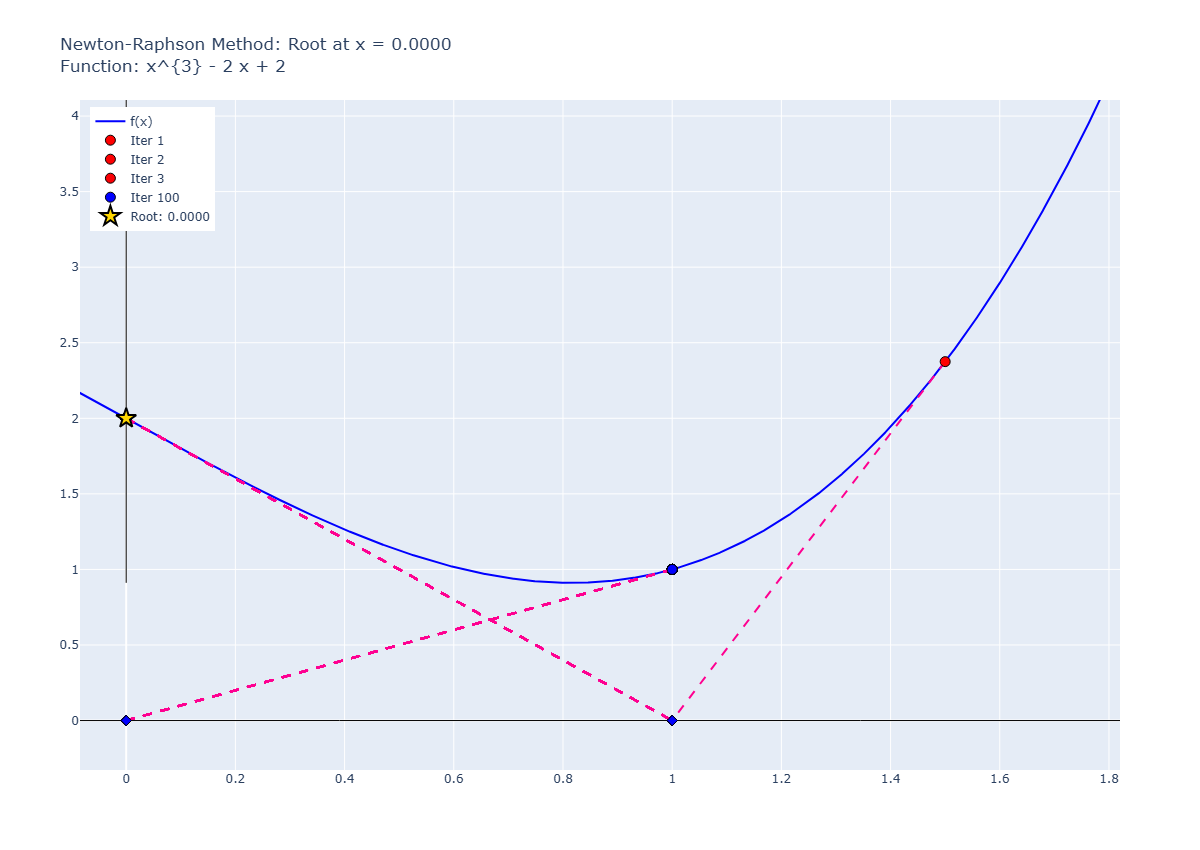
\includegraphics[width=1\textwidth]{Imagens/pitfalls/03/x3_2x_2_10.png}
    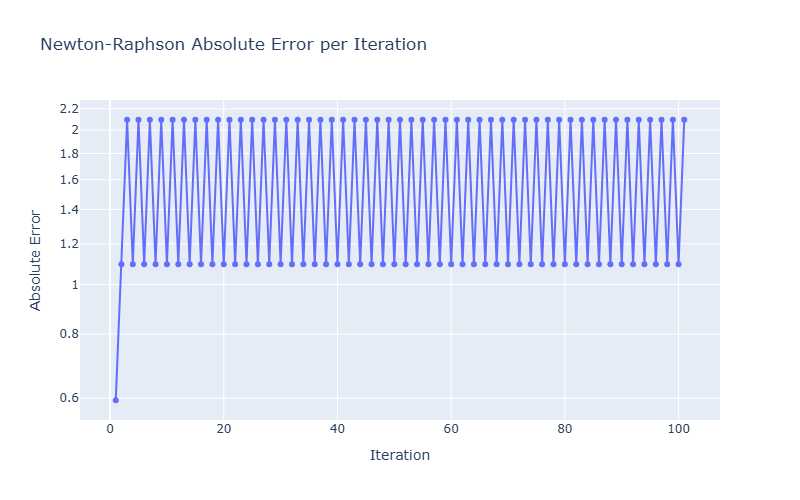
\includegraphics[width=1\textwidth]{Imagens/pitfalls/03/err_x3_2x_2_10.png}
    \caption{Cilada de ponto de Mínimo presa.}
    \label{fig:ciladaMinMax_B}
\end{figure}

\begin{center}
    \small
    \begin{tabular}{|c|c|c|c|}
        \hline
        Iteração & Valor de $x_k$            & $f(x)$                       & Erro $e_k$            \\
        \hline
        1        & $x = 1.50000000000000000$ & $f(x) = 2.37500000000000000$ & $0.59455148154232651$ \\
        \hline
        2        & $x = 1.00000000000000000$ & $f(x) = 1.00000000000000000$ & $1.09455148154232651$ \\
        \hline
        3        & $x = 0.00000000000000000$ & $f(x) = 2.00000000000000000$ & $2.09455148154232651$ \\
        \hline
        4        & $x = 1.00000000000000000$ & $f(x) = 1.00000000000000000$ & $1.09455148154232651$ \\
        \hline
        5        & $x = 0.00000000000000000$ & $f(x) = 2.00000000000000000$ & $2.09455148154232651$ \\
        \hline
        $\vdots$ & $\vdots$                  & $\vdots$                     & $\vdots$              \\
        \hline
        100      & $x = 1.00000000000000000$ & $f(x) = 1.00000000000000000$ & $1.09455148154232651$ \\
        \hline
        101      & $x = 0.00000000000000000$ & $f(x) = 2.00000000000000000$ & $2.09455148154232651$ \\
        \hline
    \end{tabular}
    \label{tab:ciladaMinMax_B}
\end{center}

\subsubsection{Caso 3: Proximidade a Pontos de Inflexão}
Pontos de inflexão também podem causar problemas no método de Newton. Se a raiz
estiver próxima de um ponto de inflexão da função \(f(x)\), onde a derivada
segunda muda de sinal, o método pode não convergir para a raiz desejada. Isso
acontece porque a tangente à curva nesse ponto pode não fornecer uma boa
aproximação da raiz, resultando em saltos grandes na iteração e afastando-a da
raiz.
\begin{figure}[H]
    \centering
    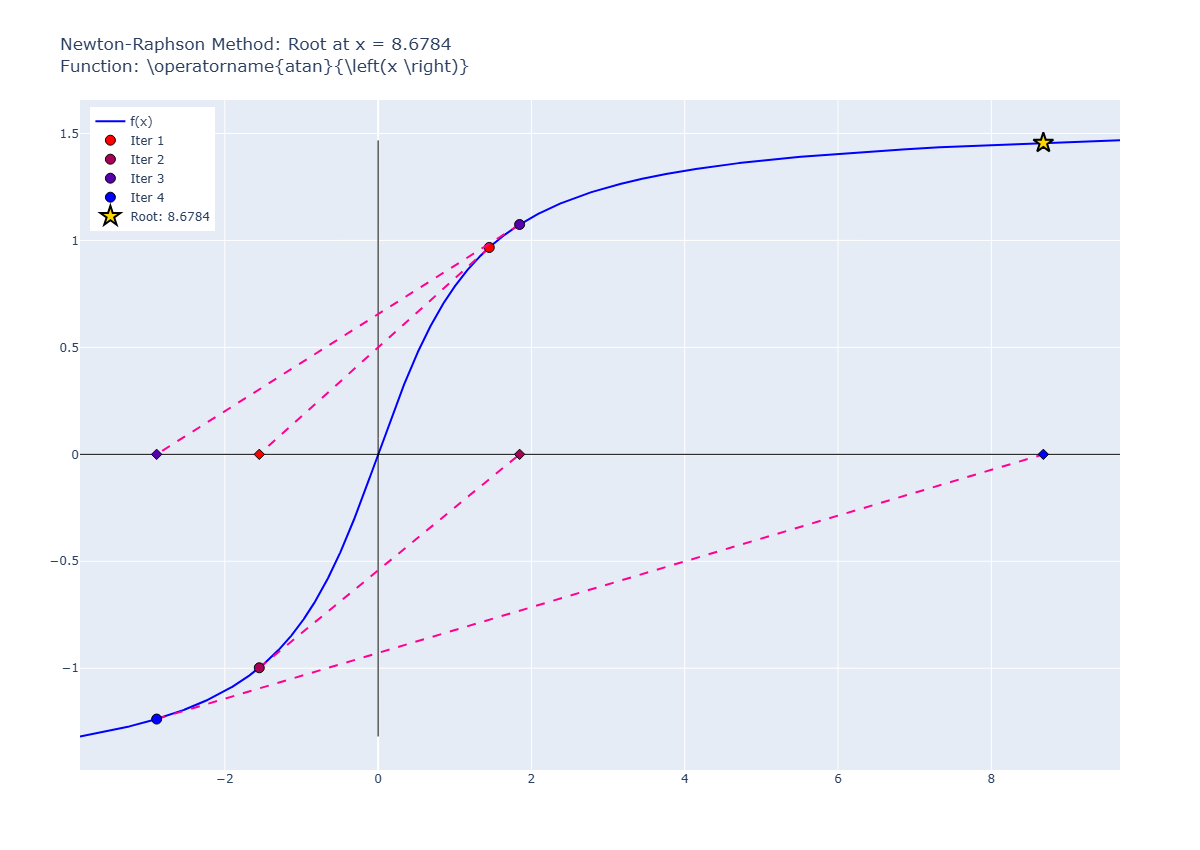
\includegraphics[width=1\textwidth]{Imagens/pitfalls/04/arctg.png}
    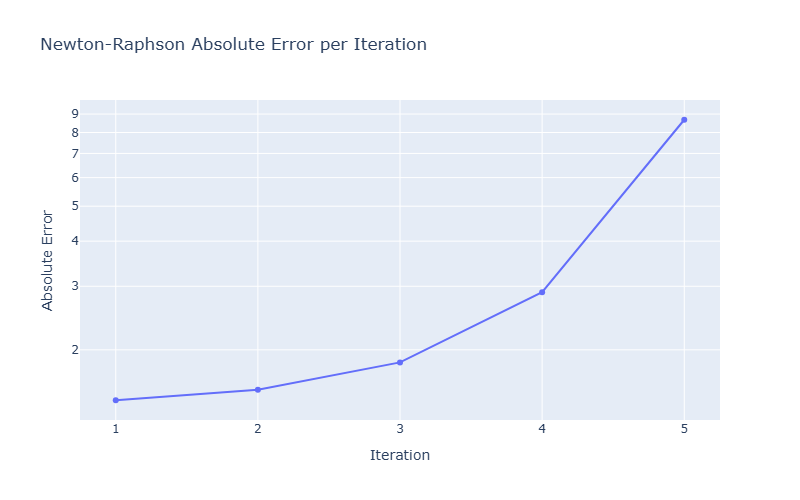
\includegraphics[width=1\textwidth]{Imagens/pitfalls/04/err_arctg.png}
    \caption{Cilada de ponto de Inflexão.}
    \label{fig:ciladaPontoInflexao}
\end{figure}
Ao analisar o gráfico é possivel notar que conforme as iterações avançam, a função se afasta da raiz, resultando em saltos cada vez maiores. Isso ocorre porque a tangente à curva no ponto de inflexão não fornece uma boa aproximação da raiz, levando o método a divergir.

\begin{center}
    \small
    \begin{tabular}{|c|c|c|c|}
        \hline
        Iteração & Valor de $x_k$             & $f(x)$                        & Erro $e_k$            \\
        \hline
        1        & $x = 1.44999999999999996$  & $f(x) = 0.96704699339746025$  & $1.44999999999999996$ \\
        \hline
        2        & $x = -1.55026329701562049$ & $f(x) = -0.99790755802460773$ & $1.55026329701562049$ \\
        \hline
        3        & $x = 1.84593175119723552$  & $f(x) = 1.07432318743154331$  & $1.84593175119723552$ \\
        \hline
        4        & $x = -2.88910905408613594$ & $f(x) = -1.23757558204700402$ & $2.88910905408613594$ \\
        \hline
        5        & $x = 8.67844942653632145$  & $f(x) = 1.45607432393228908$  & $8.67844942653632145$ \\
        \hline
    \end{tabular}
    \label{tab:ciladaPontoInflexao}
\end{center}

\subsubsection{Caso 4: Derivada próxima de zero}
Além disso, quando a derivada de uma iteração é muito próxima de zero, o metodo
vai ter dificuldades em convergir. Isso ocorre porque a divisão por zero ou por
um número muito pequeno pode resultar em saltos grandes na iteração,
afastando-a da raiz.
\begin{figure}[H]
    \centering
    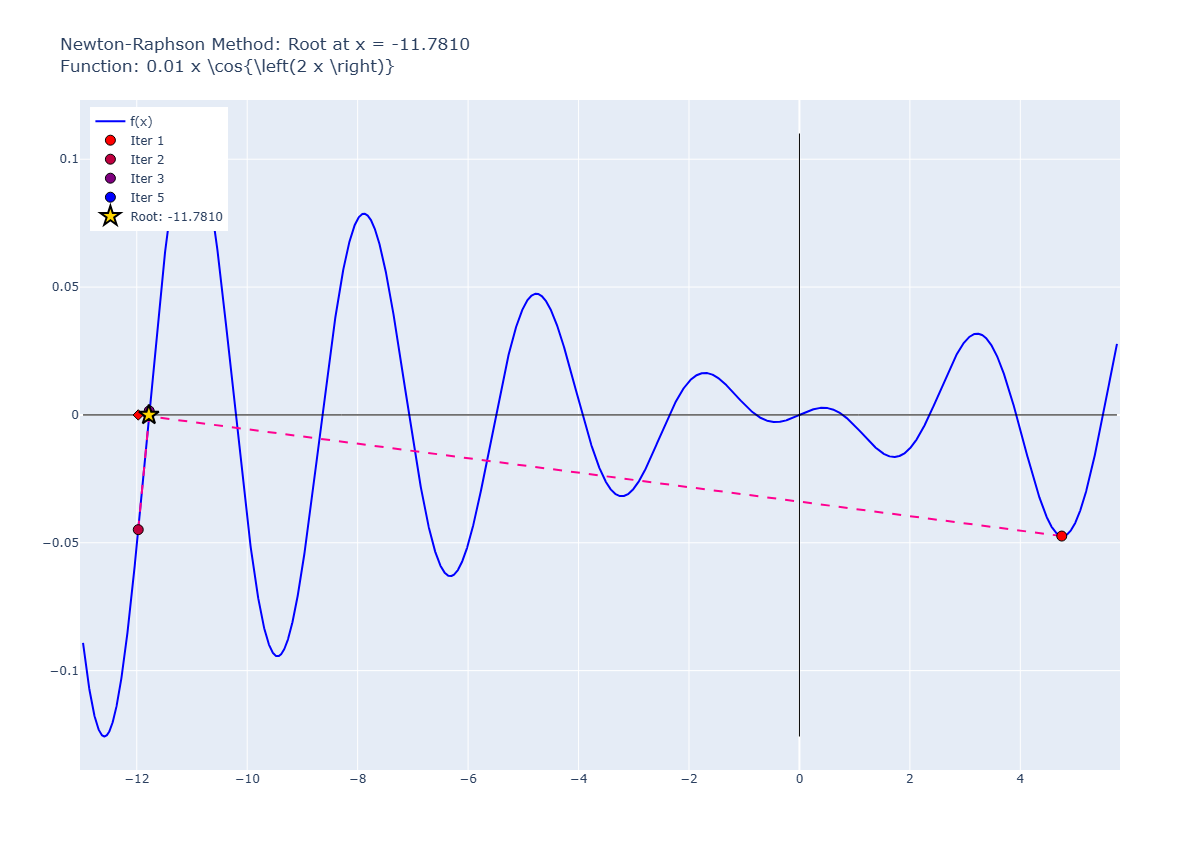
\includegraphics[width=1\textwidth]{Imagens/pitfalls/06/slope_near_zero.png}
    \caption{Cilada de derivada próxima de zero.}
    \label{fig:ciladaDerivadaProximaZero}
\end{figure}
Podemos perceber que a inclinação da tangente à curva em torno da raiz é muito próxima de zero, o que resulta em um salto enorme, levando a iteração para longe da raiz mais próxima.

\begin{center}
    \small
    \begin{tabular}{|c|c|c|}
        \hline
        Iteração & Valor de $x_k$              & $f(x)$                        \\
        \hline
        1        & $x = 4.75000000000000000$   & $f(x) = -0.04736567741932798$ \\
        \hline
        2        & $x = -11.97301255116330410$ & $f(x) = -0.04486365737362013$ \\
        \hline
        3        & $x = -11.77429070649470333$ & $f(x) = 0.00157340920400228$  \\
        \hline
        4        & $x = -11.78097664313937010$ & $f(x) = -0.00000098775893849$ \\
        \hline
        5        & $x = -11.78097245096321544$ & $f(x) = -0.00000000000035126$ \\
        \hline
        6        & $x = -11.78097245096172507$ & $f(x) = -0.00000000000000010$ \\
        \hline
    \end{tabular}
    \label{tab:ciladaNRDerivadaProximaZero}
\end{center}
Em resumo, para evitar os problemas apresentados — como convergência lenta, divergência ou oscilação — é fundamental analisar previamente o comportamento da função. Recomenda-se identificar regiões próximas a pontos de máximo, mínimo, inflexão, derivadas próximas de zero e raízes múltiplas. Além disso, a escolha do chute inicial $x_0$ deve ser feita de modo criterioso: o ponto deve estar suficientemente próximo da raiz desejada e em uma região onde a derivada não seja nula ou muito pequena, garantindo assim maior probabilidade de convergência rápida e correta do método.

\begin{comment}
{Derivada nula:} Se a derivada \(f'(x_k)\) for zero ou muito próxima de zero, a iteração pode divergir ou levar a resultados imprecisos. Isso ocorre porque a divisão por zero ou por um número muito pequeno pode resultar em saltos grandes na iteração, afastando-a da raiz.
    {Ponto de inflexão:} Se o ponto inicial \(x_0\) estiver próximo de um ponto de inflexão da função \(f(x)\), onde a derivada muda de sinal, o método pode não convergir para a raiz desejada. Isso acontece porque a tangente à curva nesse ponto pode não fornecer uma boa aproximação da raiz.
    {Raízes múltiplas:} Se a função \(f(x)\) tiver uma raiz múltipla, ou seja, uma raiz onde a função toca o eixo x mas não o cruza, o método de Newton pode convergir lentamente ou até mesmo divergir.
    {Escolha inadequada de \(x_0\):} Se o ponto inicial \(x_0\) estiver muito longe da raiz ou em uma região onde a função não é bem comportada, o método pode não convergir ou convergir para uma raiz errada. A escolha de um bom ponto inicial é crucial para o sucesso do método
\end{comment}

\section{Método de Newton-Raphson N-dimensional}
O método de Newton-Raphson pode ser estendido para resolver sistemas de
equações não lineares em múltiplas variáveis. Um sistema de equações não
lineares ser representado da seguinte maneira:
\begin{equation*}
    \begin{cases}
        f_1(x_1, x_2, \ldots, x_n) = 0             \\
        f_2(x_1, x_2, \ldots, x_n) = 0             \\
        \qquad \qquad \vdots \qquad \qquad  \vdots \\
        f_n(x_1, x_2, \ldots, x_n) = 0
    \end{cases}
\end{equation*}
onde  \(f_i \) são as funções não lineares e \(x_i\) são as variáveis desconhecidas.

Podemos escrever esse sistema de \textbf{\(n\)} variáveis como uma função
\textbf{\(F : \mathbb{R}^n \rightarrow \mathbb{R}^n\)}' da seguinte forma:
\begin{equation*}
    F((x_1, x_2, \ldots, x_n)) = (f_1(x_1, x_2, \ldots, x_n), f_2(x_1, x_2, \ldots, x_n), \ldots, f_n(x_1, x_2, \ldots, x_n))^{t}
\end{equation*}
Portanto, de forma mais compacta, o sistema pode ser escrito na forma vetorial como \textbf{\(F(X) = 0\)}, onde \textbf{\(F\)} é uma função vetorial e \(X\) é um vetor de variáveis.

\subsection{Definições}

Durante a construção do método de Newton-Raphson unidimensional
(\ref{sec:NR1d}), definimos a função de iteração
\begin{equation*}
    \varphi(x) = x - {A(x)}{f(x)}.
\end{equation*}
com isso achamos que a função \(A(x)\) que satisfazia \(\varphi'(\xi) = 0\) é \(A(x) = \frac{-1}{f'(x)}\) desde que \(f'(x) \neq 0\).
Similarmente, para o caso n-dimensional, generalizamos a função de iteração como
\begin{equation*}
    G(\xb) = x - A(x)^{-1} F(x)
\end{equation*}
em que \(A(x)\) é a matriz não singular que satisfaz \(G'(\xi) = 0\). A matriz \(A(x)\) pode ser representada como
\begin{equation}\label{matA}
    A(x) =
    \begin{bmatrix}
        a_{11}(x) & a_{12}(x) & \ldots & a_{1n}(x) \\
        a_{21}(x) & a_{22}(x) & \ldots & a_{2n}(x) \\
        \vdots    & \vdots    & \ddots & \vdots    \\
        a_{n1}(x) & a_{n2}(x) & \ldots & a_{nn}(x)
    \end{bmatrix}
\end{equation}
onde cada entrada  \(a_{ij}(x)\) é uma função de   \(\mathbb{R}^n \rightarrow  \mathbb{R}\). Seja \(b_{ij}\) as entradas da matriz inversa \(A^{-1}(x)\). As funções coordenadas  $g_{i}(\xb)$ são da forma

\begin{equation}
    g_{i}(\xb) = x_i - \sum_{j=1}^{n} b_{ij}(x) f_j(x)
\end{equation}
e
\begin{equation}\label{sumInvA}
    \frac{\partial g_i(\xb)}{\partial x_k} = \delta_{ik} - \sum_{j=1}^{n} \left( \frac{\partial b_{ij}(x)}{\partial x_k} f_j(x) + b_{ij}(x) \frac{\partial f_j(x)}{\partial x_k} \right)
\end{equation}
onde \(\delta_{ik}\) é o delta de Kronecker, que é 1 se \(i = k\) e 0 caso contrário.

\subsection{Calculo do Jacobiano}

\newtheorem*{dfNRnd}{Método de Newton-Raphson N-dimensional}
\begin{dfNRnd}
    \begin{prop}
        Seja $\mathbf{p}$ um ponto fixo de \(\mathbb{G}\). Se existe um \(\delta > 0\) tal que

        \begin{itemize} %\label{teoMPF}
            \item[i)] $\frac{\partial g_i}{\partial x_j}$ é contínua em uma vizinhança
                  $N_{\delta} = \{x \in \mathbb{R}^n : ||x - p|| < \delta\}$ para todo $i, j = 1,
                      2, \ldots, n$
            \item [ii)] $\frac{\partial^2 \mathbb{G}_i}{\partial x_j \partial x_k}$ é contínua e $|\frac{\partial^2g_i(x)}{\partial x_j \partial x_k}| \leq $M$ $
            \item [iii)] $\frac{\partial g_i(p)}{\partial x_k} = 0$, para todo $i = 1,2, \ldots, n$
        \end{itemize}
        Então existe \(\bar{\delta} \leq \delta\) de tal forma que a sequência gerada por $x_{k+1} = \mathbb{G}(x_{k})$ converge para $\mathbf{p}$ de forma quadrática, para qualquer escolha de $x_{0}$ que satisfaz \(|| x_{0} - \mathbf{p} || \leq \bar{\delta}\)
    \end{prop}

\end{dfNRnd}
\EnzoR{Tarefa aos Matematicos: Encontrar onde isso ta demonstrado}
A demonstração é análoga à do Teorema \ref{teoNR}. E está descrita extensivamente em ref.

A partir de (\ref{sumInvA}) vamos caracterizar a matriz A. Obseve que, de \(
\frac{\partial g_i(\mathbf{p})}{\partial x_k} = 0 \) para todo $ i = 1,2,
    \ldots, n$, temos que
\begin{equation}\label{aInvs1}
    0 = 1 - \sum_{j=1}^{n} \left( b_{ij}(\mathbf{p}) \frac{\partial f_j(\mathbf{p})}{\partial x_i} \right) \ \ \text{para i = j}
\end{equation}
e
\begin{equation}\label{aInvs2}
    0 = - \sum_{j=1}^{n} \left( b_{ij}(\mathbf{p}) \frac{\partial f_j(\mathbf{p})}{\partial x_k} \right)\ \ \text{para i $\neq$ j}.
\end{equation}
A matriz Jacobiana \(J\) de \(F\) é a matriz das derivadas dada a seguir:
\begin{equation}
    J(\mathbf{p}) =
    \begin{bmatrix}
        \frac{\partial f_1(\mathbf{p})}{\partial x_1} & \frac{\partial f_1(\mathbf{p})}{\partial x_2} & \ldots & \frac{\partial f_1(\mathbf{p})}{\partial x_n} \\
        \frac{\partial f_2(\mathbf{p})}{\partial x_1} & \frac{\partial f_2(\mathbf{p})}{\partial x_2} & \ldots & \frac{\partial f_2(\mathbf{p})}{\partial x_n} \\
        \vdots                                        & \vdots                                        & \ddots & \vdots                                        \\
        \frac{\partial f_n(\mathbf{p})}{\partial x_1} & \frac{\partial f_n(\mathbf{p})}{\partial x_2} & \ldots & \frac{\partial f_n(\mathbf{p})}{\partial x_n}
    \end{bmatrix}
\end{equation}
As condições (\ref{aInvs1}) e (\ref{aInvs2}) implicam que
\begin{align*}
    A(\mathbf{p})^{-1} J(\mathbf{p})               & = I               \\[6pt]
    A(\mathbf{p}) A(\mathbf{p})^{-1} J(\mathbf{p}) & = A(\mathbf{p}) I \\[6pt]
    I J(\mathbf{p})                                & = A(\mathbf{p})   \\[6pt]
    J(\mathbf{p})                                  & = A(\mathbf{p})
\end{align*}
Portanto, uma escolha natural para \(A(x)\) é a matriz Jacobiana \(J(x)\) de \(F\). Assim, a função de iteração do método de Newton-Raphson n-dimensional é dada por
\begin{equation}
    G(\xb) = x - J(x)^{-1} F(x).
\end{equation}
A sequência iterativa do MNR n-dimensional é
\begin{equation}\label{seqIterNRndim}
    x_{k+1} = x_k - J(x_k)^{-1} F(x_k)
\end{equation}
onde \(\xb_k\) é a aproximação atual da solução, \(J(x_k)\) é a matriz Jacobiana avaliada em \(x_k\), e \(F(\xb_k)\) é o vetor de funções avaliado em \(x_k\). É esperado que a sequência \(\{x_k\}\) convirja, \textbf{quadraticamente}, para a solução do sistema de equações não lineares, desde que o chute inicial \(x_0\) esteja suficientemente próximo da solução e que a matriz Jacobiana avaliada em \(J(x_k)\) seja invertível nesse ponto.
Vejamos um exemplo para n = 2. Considere o sistema de equações não lineares:
\begin{equation*}
    \begin{cases}
        x^2 + y^2 - 4 = 0 \\
        x^2 - y - 1 = 0
    \end{cases}
\end{equation*}
Podemos definir a função \(F : \mathbb{R}^2 \rightarrow \mathbb{R}^2\) como
\begin{equation*}
    F((x, y)) = \begin{bmatrix}
        x^2 + y^2 - 4 \\
        x^2 - y - 1
    \end{bmatrix}
\end{equation*}
A matriz Jacobiana \(J(x, y)\) de \(F\) é dada por
\begin{equation*}
    J((x, y)) = \begin{bmatrix}
        \frac{\partial ( x^2 + y^2 - 4 )}{\partial x} & \frac{\partial ( x^2 + y^2 - 4 )}{\partial y} \\
        \frac{\partial ( x^2 - y - 1 )}{\partial x}   & \frac{\partial ( x^2 - y - 1 )}{\partial y}
    \end{bmatrix}
\end{equation*}
\begin{equation*}
    J((x, y)) = \begin{bmatrix}
        2x & 2y \\
        2x & -1
    \end{bmatrix}
\end{equation*}
A iteração do método de Newton-Raphson n-dimensional é então dada por
\begin{align*}
    \begin{bmatrix}
        x_{k+1} \\
        y_{k+1}
    \end{bmatrix}
     & =
    \begin{bmatrix}
        x_k \\
        y_k
    \end{bmatrix} - J((x_k, y_k))^{-1} F((x_k, y_k)) \\[12pt]
     & =
    \begin{bmatrix}
        x_k \\
        y_k
    \end{bmatrix} -
    \begin{bmatrix}
        2x_k & 2y_k \\
        2x_k & -1
    \end{bmatrix}^{-1}
    \begin{bmatrix}
        x_k^2 + y_k^2 - 4 \\
        x_k^2 - y_k - 1
    \end{bmatrix}                                \\[12pt]
     & =
    \begin{bmatrix}
        x_k \\
        y_k
    \end{bmatrix} -
    \frac{1}{-2x_k - 4 x_k y_k }
    \begin{bmatrix}
        -1    & -2y_k \\
        -2x_k & 2x_k
    \end{bmatrix}
    \begin{bmatrix}
        x_k^2 + y_k - 4 \\
        x_k^2 - y_k - 1
    \end{bmatrix}
\end{align*}

Vamos escolher um chute inicial \( (x_0, y_0) = (2, 1) \) e aplicar o método
iterativamente:
\begin{center}
    \begin{tabular}{|c|c|c|}
        \hline
        Iteração & $x_k$              & $y_k$              \\
        \hline
        0        & 2.0000000000000000 & 1.0000000000000000 \\
        1        & 1.5000000000000000 & 0.2500000000000000 \\
        2        & 1.3095238095238095 & 0.7142857142857143 \\
        3        & 1.2727272727272727 & 0.6181818181818182 \\
        4        & 1.2679491924311228 & 0.6180339887498950 \\
        5        & 1.2679491924311228 & 0.6180339887498950 \\
        \hline
    \end{tabular}
\end{center}

Após algumas iterações, o método converge para a solução aproximada \( (x, y)
\approx (1.2679491924311228, 0.618033988749895) \), que satisfaz o sistema de
equações não lineares. Do ponto de vista computacional, calcular explicitamente
a inversa da matriz Jacobiana pode ser ineficiente e numericamente instável,
especialmente para sistemas de grande porte. Por isso, a sequência iterativa
(\ref{seqIterNRndim}) é normalmente reescrita de forma mais eficiente, evitando
a inversão direta da matriz. Introduz-se uma variável auxiliar $\gamma$ que
representa a solução do sistema linear:

\begin{equation*}
    J(x_k)\,\gamma = -F(x_k)
\end{equation*}

Assim, a atualização da aproximação é feita por
\begin{equation*}
    x_{k+1} = x_k + \gamma
\end{equation*}

Dessa forma, em cada iteração, resolve-se um sistema linear envolvendo a matriz
Jacobiana, o que é computacionalmente mais eficiente e estável do que calcular
sua inversa.
\begin{align*}
    \gamma        & = - J(x_k)^{-1} F(x_k)       \\
    J(x_k) \gamma & = J(x_k) J(x_k)^{-1} F(x_k)  \\
    J(x_k) \gamma & = - F(x_k) \label{auxNRndim}
\end{align*}
Subistituindo $\gamma$ em ( \ref{seqIterNRndim} ) temos
\begin{equation*}
    x_{k+1} = x_k + \gamma
\end{equation*}

\newpage

\subsection{Números Complexos e Plano Complexo}

A compreensão dos funcionamento de números complexos durante o estudo de
métodos para solução de raízes de funções é motivida pelo seguinte teorema.
\begin{tfa}
    Todo polinômio não constante com coeficientes complexos possui, pelo menos, uma raiz complexa.

    Seja $P(z)$ um polinômio de grau $n \ge 1$ da forma:
    \[ P(z) = a_n z^n + a_{n-1} z^{n-1} + \dots + a_1 z + a_0 \]
    em que os coeficientes $a_i \in \mathbb{C}$ para todo $i = 0, 1, \dots, n$ e
    $a_n \neq 0$. Então, existe pelo menos um número $z_0 \in \mathbb{C}$ tal que:
    \[ P(z_0) = 0 \]
\end{tfa}

\begin{corolario}[Decomposição em $n$ Raízes]
    Como consequência direta do TFA, utilizando o teorema do resto e a divisão polinomial indutiva, demonstra-se que todo polinômio de grau $n$ possui exatamente $n$ raízes complexas (contadas com suas respectivas multiplicidades).

    Dessa forma, $P(z)$ pode ser completamente fatorado em $\mathbb{C}$ como:
    \[ P(z) = a_n (z - z_1)(z - z_2) \dots (z - z_n) \]
    em que $z_1, z_2, \dots, z_n \in \mathbb{C}$ são as raízes do polinômio.
\end{corolario}

Definimos um novo número, representado por $i = \sqrt{-1}$. O conjunto dos
números complexos $\mathbb{C}$ é o conjunto de todos os números da forma $z = a
    + bi$ em que $a$ é a parte real e $b$ é a parte imaginária do número complexo
$z$. O plano complexo é uma representação bidimensional dos números complexos,
em que o eixo horizontal representa a parte real e o eixo vertical representa a
parte imaginária.
\begin{figure}[H]
    \centering
    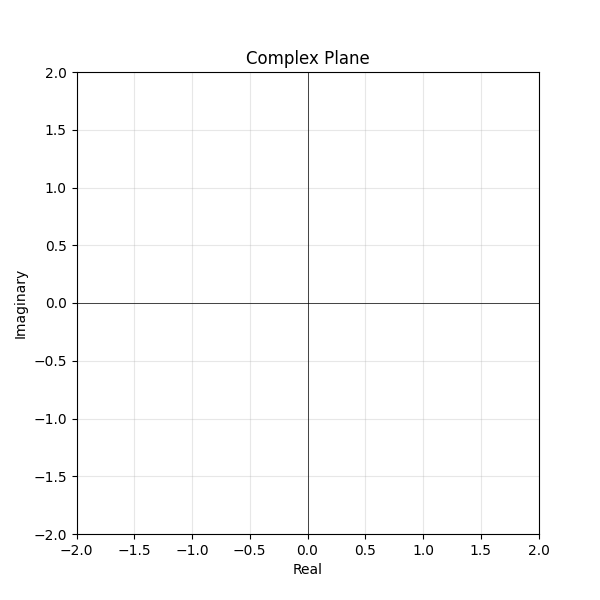
\includegraphics[width=.5\textwidth]{Imagens/complexPlane/complex_plane_axes.png}
    \caption{Plano Complexo}
    \label{fig:complexPlane}
\end{figure}
\begin{figure}[H]
    \centering
    \begin{minipage}{0.48\textwidth}
        \centering
        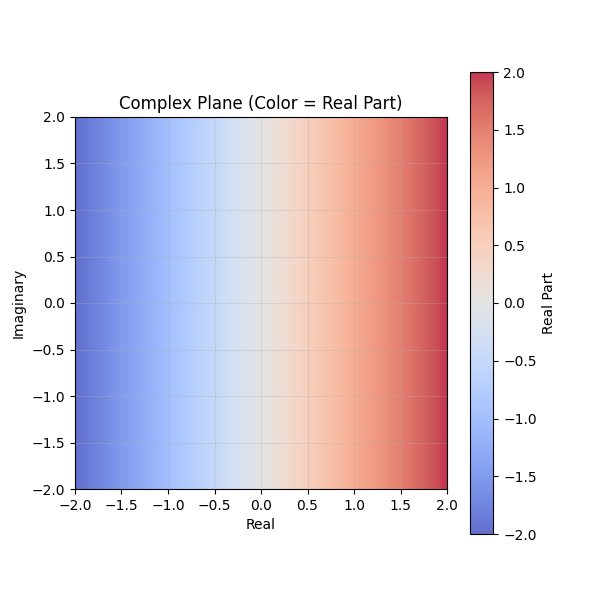
\includegraphics[width=\textwidth]{Imagens//complexPlane/complex_plane_real_part.png}
        \caption*{Parte Real}
    \end{minipage}\hfill
    \begin{minipage}{0.48\textwidth}
        \centering
        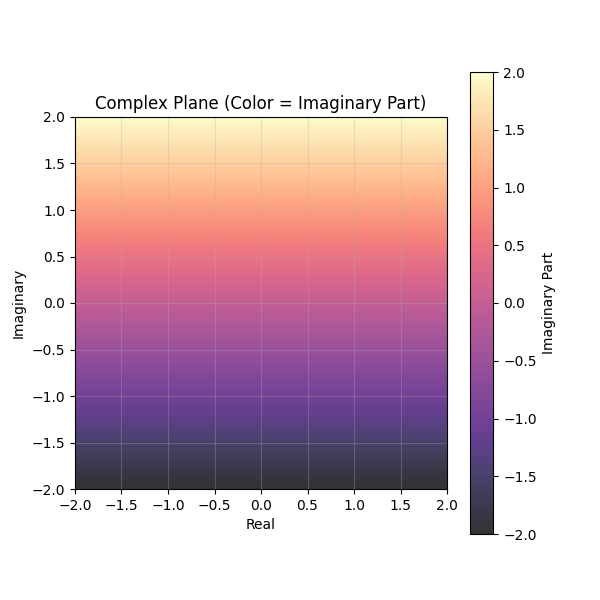
\includegraphics[width=\textwidth]{Imagens//complexPlane/complex_plane_imaginary_part.png}
        \caption*{Parte Imaginária}
    \end{minipage}\\[1em]
    \begin{minipage}{0.48\textwidth}
        \centering
        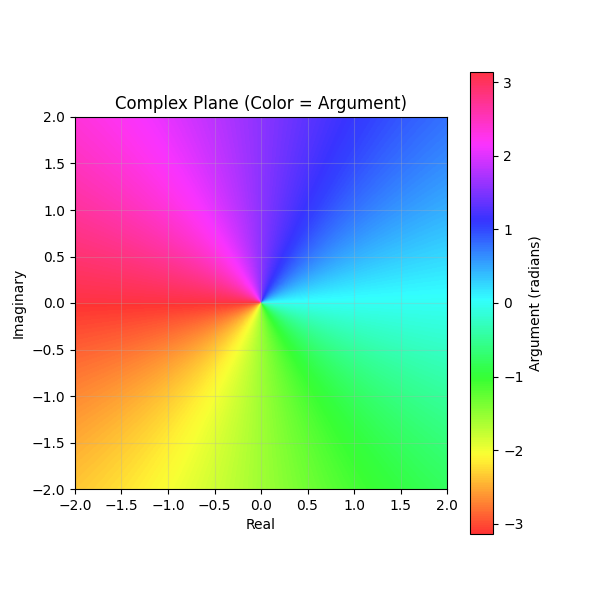
\includegraphics[width=\textwidth]{Imagens//complexPlane/complex_plane_argument.png}
        \caption*{Parte Angular}
    \end{minipage}\hfill
    \begin{minipage}{0.48\textwidth}
        \centering
        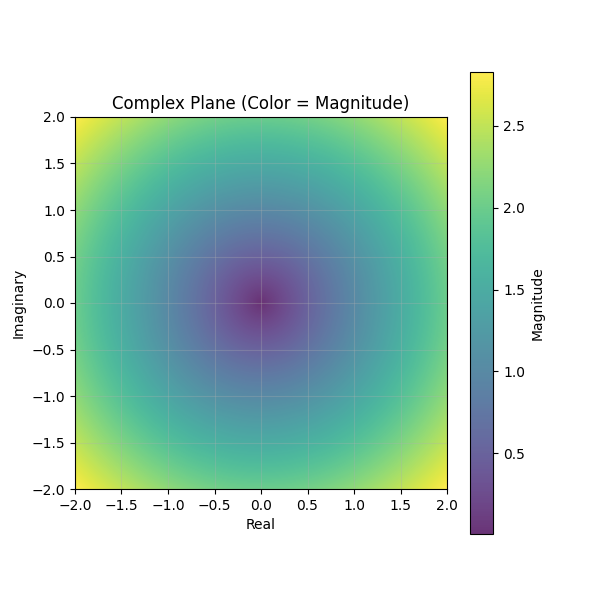
\includegraphics[width=\textwidth]{Imagens//complexPlane/complex_plane_magnitude.png}
        \caption*{Parte Magnitude}
    \end{minipage}
    \caption{Propriedades dos Números Complexos}
    \label{fig:complexPlaneProps}
\end{figure}

\subsection{Fractais de Newton}\label{sec:nrfractals}
A aplicação do método de Newton-Raphson a funções complexas \(f: \mathbb{C}
\rightarrow \mathbb{C}\) sobre o plano \textit{\textbf{Plano Complexo}} gera os
\textbf{Fractais de Newton}. Os fractais de Newton são objetos interessantes a
serem analisados para obter uma compreensão mais profunda do comportamento do
método.

A fórmula de iteração é semelhante à do caso para funções reais, mas agora
\(z\) é um número complexo:
\begin{equation*}
    z_{n+1} = z_n - \frac{f(z_n)}{f'(z_n)}
\end{equation*}
em que \(z_n\) é a aproximação atual, \(f(z_n)\) é o valor da função no ponto \(z_n\), e \(f'(z_n)\) é a derivada da função no ponto \(z_n\).

A ideia básica para gerar um fractal de Newton é aplicar o método de
Newton-Raphson a cada ponto em uma região do plano complexo e colorir o ponto
com base na raiz para a qual ele converge e o número de iterações que levou
para convergir. Se um ponto não convergir para nenhuma raiz dentro da
tolerância estabelecida, ele é colorido de uma forma diferente. Nos gráficos
utilizados nessa seção, quanto mais escura uma cor, mais tempo levou para
convergir, e preto indica que não convergiu. \TODO{Adicionar legenda com escala
    de brilho e cores.}

\begin{figure}[H]
    \centering
    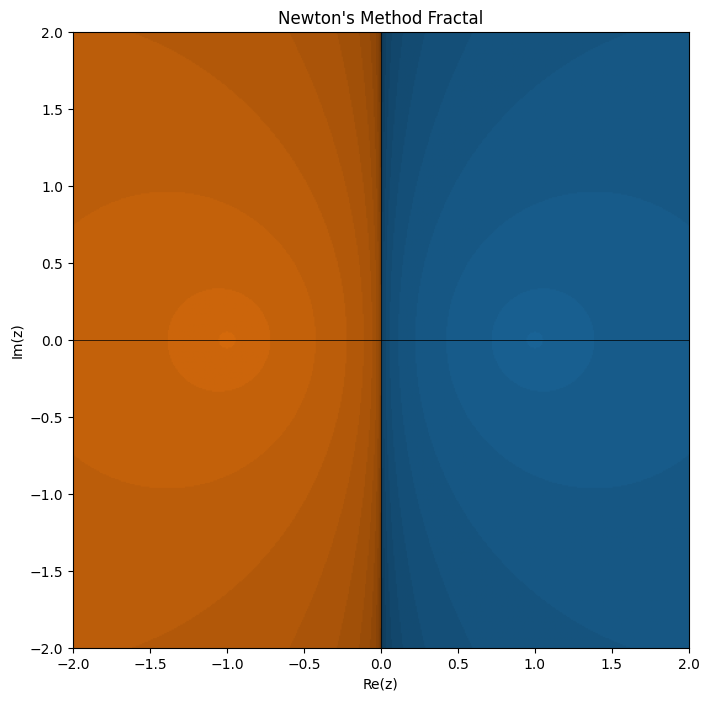
\includegraphics[width=1\textwidth]{Imagens/nr2d_fractals/unit_roots/unitroot2.png}
    \caption{Fractais de Newton -- 2 Unidades da raiz.}
    \label{fig:fractaisnr_unitroots2}
\end{figure}

\begin{figure}[H]
    \centering
    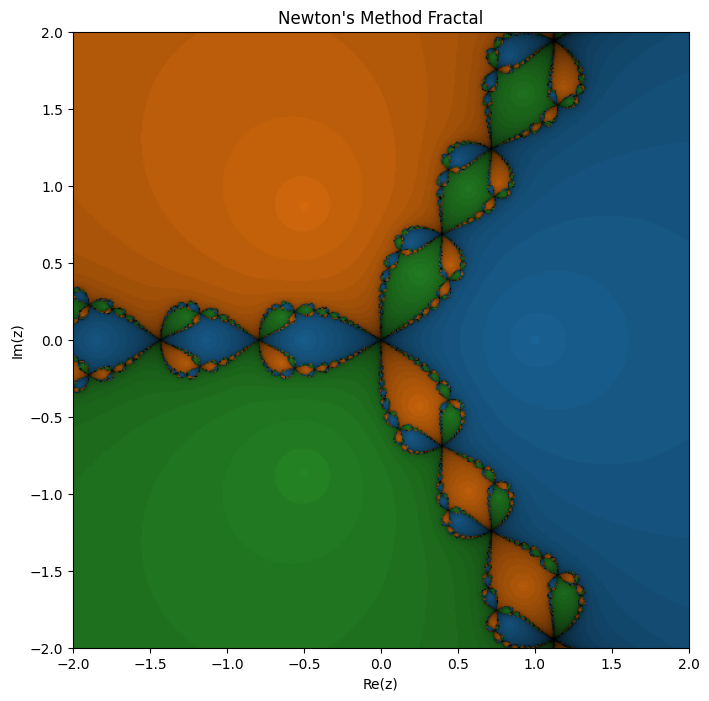
\includegraphics[width=1\textwidth]{Imagens/nr2d_fractals/unit_roots/unitroot3.png}
    \caption{Fractais de Newton - 3 Unidades da raiz.}
    \label{fig:fractaisnr_unitroots3}
\end{figure}

\begin{figure}[H]
    \centering
    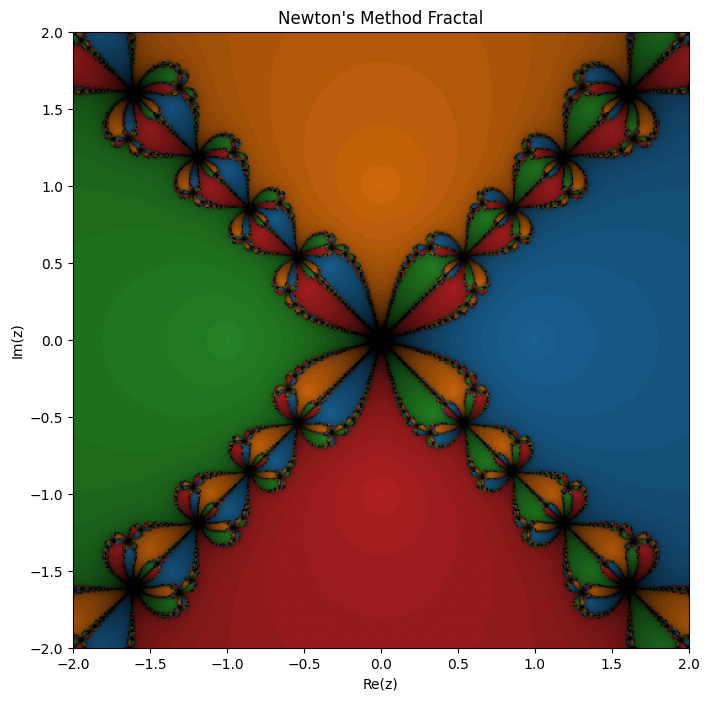
\includegraphics[width=1\textwidth]{Imagens/nr2d_fractals/unit_roots/unitroot4.png}
    \caption{Fractais de Newton - 4 Unidades da raiz.}
    \label{fig:fractaisnr_unitroots4}
\end{figure}

\begin{figure}[H]
    \centering
    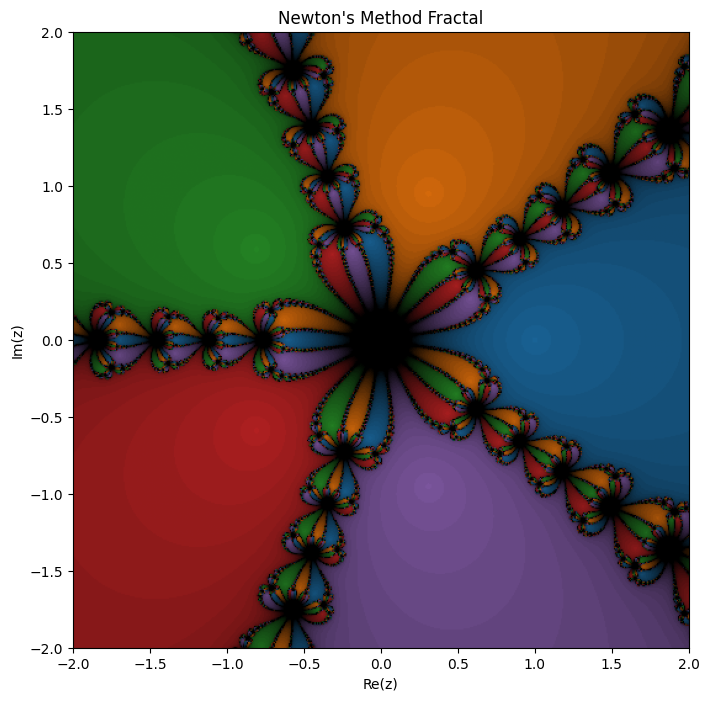
\includegraphics[width=1\textwidth]{Imagens/nr2d_fractals/unit_roots/unitroot5.png}
    \caption{Fractais de Newton - 5 Unidades da raiz.}
    \label{fig:fractaisnr_unitroots5}
\end{figure}

\begin{figure}[H]
    \centering
    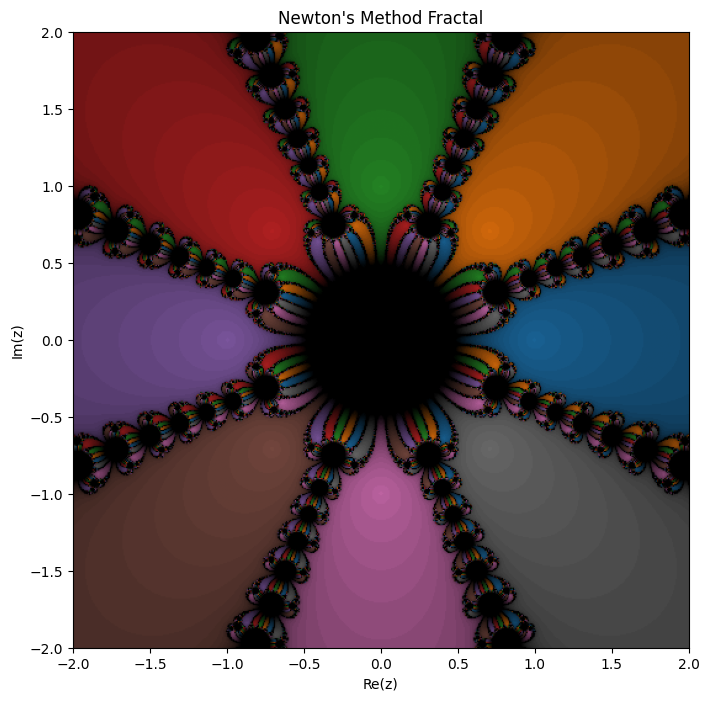
\includegraphics[width=1\textwidth]{Imagens/nr2d_fractals/unit_roots/unitroot8.png}
    \caption{Fractais de Newton - 8 Unidades da raiz.}
    \label{fig:fractaisnr_unitroots8}
\end{figure}

\begin{figure}[H]
    \centering
    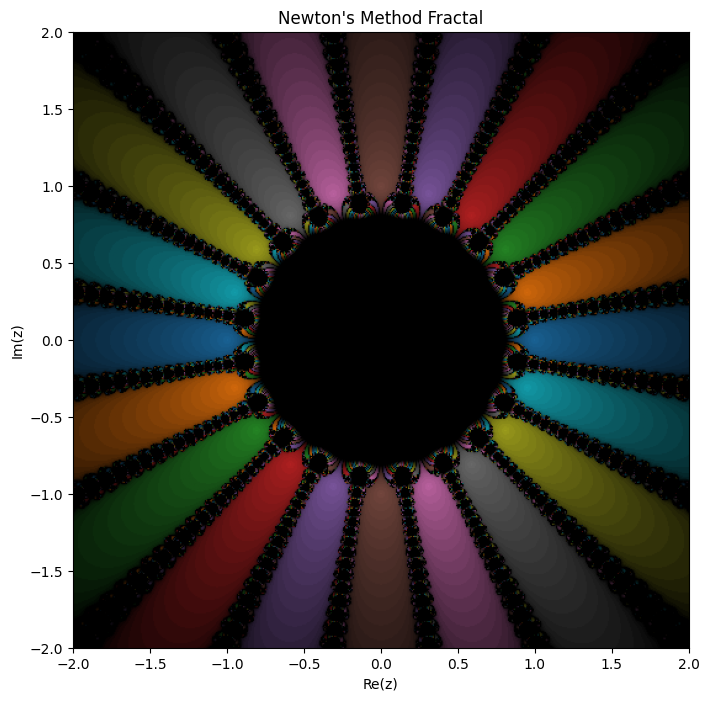
\includegraphics[width=1\textwidth]{Imagens/nr2d_fractals/unit_roots/unitroot20.png}
    \caption{Fractais de Newton - 20 Unidades da raiz.}
    \label{fig:fractaisnr_unitroots20}
\end{figure}

\begin{figure}[H]
    \centering
    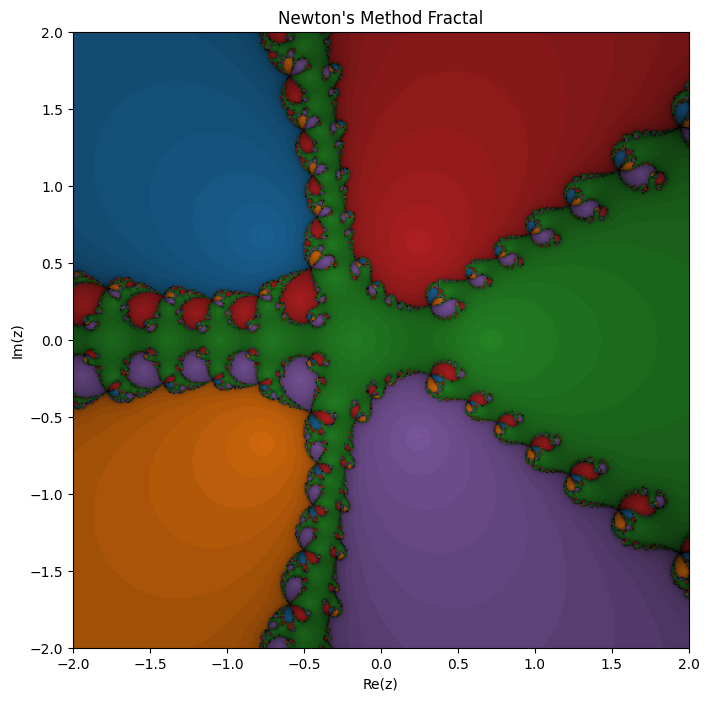
\includegraphics[width=1\textwidth]{Imagens/nr2d_fractals/polinomials/nrfractal_polinomio.png}
    \caption{Fractais de Newton - Polinomio ABCD.}
    \label{fig:fractaisnr_polinomials1}
\end{figure}

\begin{figure}[H]
    \centering
    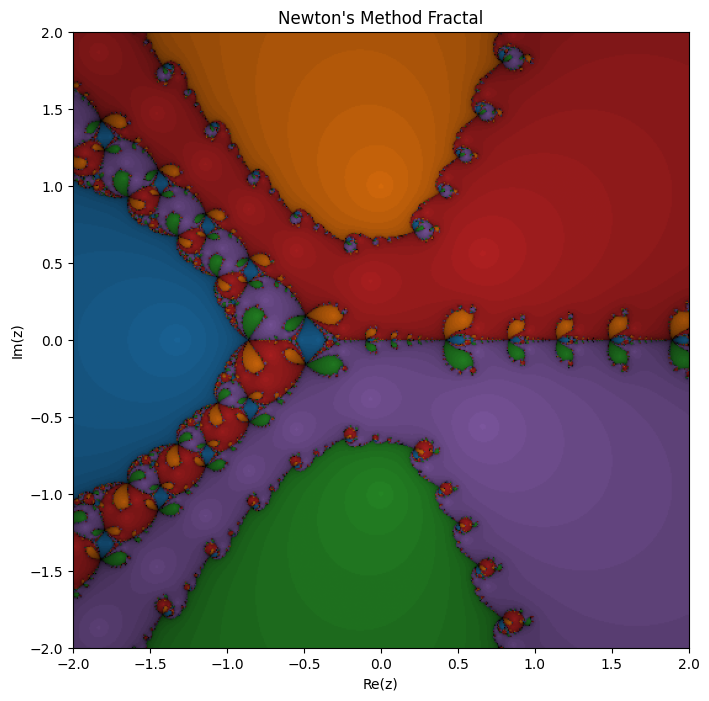
\includegraphics[width=1\textwidth]{Imagens/nr2d_fractals/polinomials/nrfractal_polinomio2.png}
    \caption{Fractais de Newton - Polinomio ABCD.}
    \label{fig:fractaisnr_polinomials2}
\end{figure}

\begin{figure}[H]
    \centering
    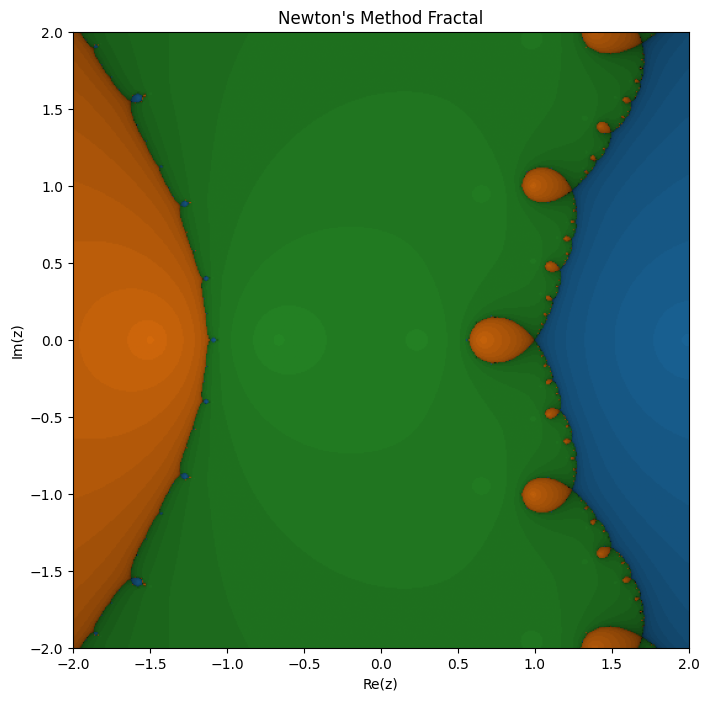
\includegraphics[width=1\textwidth]{Imagens/nr2d_fractals/polinomials/nrfractal_polinomio3.png}
    \caption{Fractais de Newton - Polinomio ABCD.}
    \label{fig:fractaisnr_polinomials3}
\end{figure}

\begin{figure}[H]
    \centering
    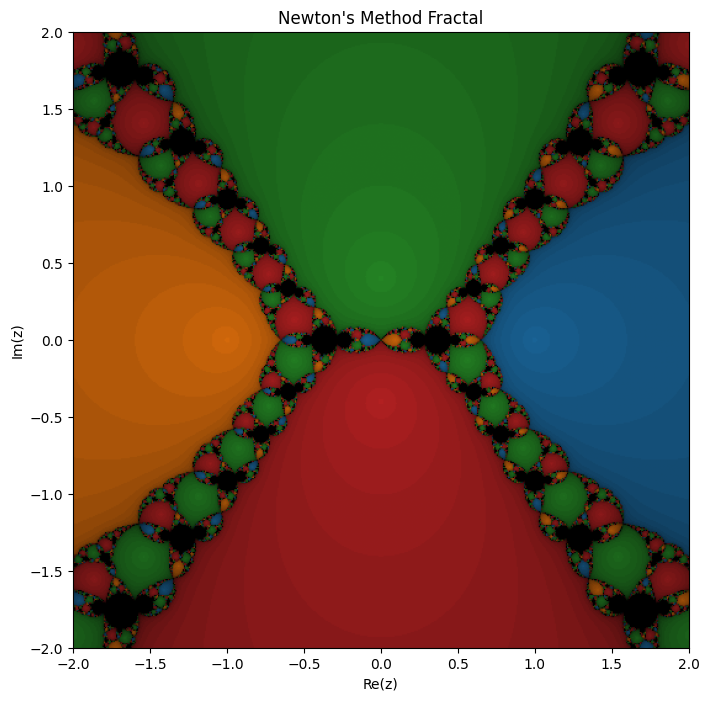
\includegraphics[width=1\textwidth]{Imagens/nr2d_fractals/polinomials/nrfractal_polinomio4.png}
    \caption{Fractais de Newton - Polinomio ABCD.}
    \label{fig:fractaisnr_polinomials4}
\end{figure}
\chapter{Problemas de Valor Inicial para Equações Diferenciais Ordinárias}

\section{Equações Diferenciais Ordinárias}
Muitos dos princípios por trás das leis da natureza são relações que estão
diretamente ligadas com a taxa de variação de certas quantidades.
Matematicamente, essas relações são equações e as taxas de variação são
representadas por derivadas. Equações que envolvem derivadas são chamadas de
equações diferenciais, que em alguns casos são chamadas de \textbf{Modelos
    Matemáticos}. Equações diferenciais podem ser classificadas em dois tipos
principais: equações diferenciais ordinárias (EDOs) e equações diferenciais
parciais (EDPs). Uma equação diferencial ordinária (EDO) é uma equação que
envolve uma função desconhecida e suas derivadas em relação a uma única
variável independente. As EDOs são amplamente utilizadas para modelar fenômenos
em diversas áreas do conhecimento, como física, engenharia, biologia, economia
etc.. As EDOs podem ser classificadas de várias maneiras. Uma equação
diferencial ordinária de primeira ordem é uma equação do tipo:
\begin{equation}
    y' = F\left(t, y\right)
\end{equation}
onde $t$ é a variável independente, $y$ é a função desconhecida, e
$y'$ é a derivada de $y$ em relação a $t$.

\begin{ex}
    Considere a equação diferencial ordinária de primeira ordem
    \begin{equation*}
        \frac{dy}{dt} = sen(t).
    \end{equation*}
    A solução geral dessa EDO é dada por:
    \begin{equation*}
        y(t) = -cos(t) + C, \quad C \in \mathbb{R}
    \end{equation*}
    Essa solução representa uma família de funções que satisfazem a equação diferencial para diferentes valores da constante de integração $C$.

    \TODO{Adicionar famílias}.
\end{ex}

\section{Definição de Problema de Valor Inicial}
Um problema de valor inicial (PVI) para uma equação diferencial ordinária
consiste em encontrar uma função desconhecida $y(t)$ que satisfaça uma equação
diferencial e que atenda a uma condição inicial especificada em um ponto $t_0$.
Para a análise de existência e unicidade de soluções consideramos as condições
de Lipschitz e continuidade. Em termos gerais, um PVI pode ser formulado como:

\begin{equation}
    \begin{cases}
        y'(t) = f(t, y(t)), & t \in [a, b] \\
        y(t_0) = y_0
    \end{cases}
\end{equation}

em que $f$ é uma função dada, $y'(t)$ é a derivada de $y(t)$ em relação a $t$,
e $y_0$ é o valor inicial da função no ponto $t_0$. A solução de um PVI é uma
função $y(t)$ que satisfaz tanto a equação diferencial quanto a condição
inicial.

A existência e unicidade de soluções para PVIs são garantidas sob certas
condições, como as condições de Lipschitz e continuidade. No geral, uma solução
de uma EDO é uma família de funções, mas ao especificar uma condição inicial,
obtemos uma solução única que passa pelo ponto inicial dado.
\begin{ex}
    Seja o PVI
    \begin{equation}
        \begin{cases}
            y'(t) = sen(t) \\
            y(0) = 0
        \end{cases}
    \end{equation}
    A solução particular desse PVI é dada por:
    \begin{equation}
        y(t) = -cos(t) + 1
    \end{equation}

    \TODO{Adicionar família com PVI destacado}.
\end{ex}

\section{Métodos Numéricos para Resolver PVIs}

Existem vários métodos numéricos para resolver problemas de valor inicial para
equações diferenciais ordinárias. Neste capítulo, discutiremos alguns dos
métodos mais comuns, incluindo o método de Euler, o método de Runge-Kutta.

\subsection{Teorema de Existência e Unicidade}
O teorema de existência e unicidade para PVIs estabelece condições sob as quais
uma solução única existe para um problema de valor inicial. Essas condições
geralmente envolvem a continuidade da função $f(t, y)$ e a satisfação da
condição de Lipschitz em relação à variável $y$.

\begin{teo}[Teorema de Existência de Peano]
    Seja $f(t, y)$ uma função contínua em um retângulo fechado $R = \{(t, y) \in \mathbb{R}^2 \mid a \leq t \leq b, c \leq y \leq d\}$. Então, para qualquer ponto inicial $(t_0, y_0) \in R$, o Problema de Valor Inicial (PVI)
    \begin{equation*}
        \begin{cases}
            y'(t) = f(t, y(t)) \\
            y(t_0) = y_0
        \end{cases}
    \end{equation*}
    admite pelo menos uma solução $y(t)$ definida em um intervalo $[t_0 - h, t_0 + h] \subset [a, b]$, onde $h > 0$.
\end{teo}

\begin{prop}[Condição de Lipschitz Local]
    Seja $f(t, y)$ definida em $R$. Diz-se que $f$ satisfaz a condição de Lipschitz em relação à variável $y$ em $R$ se existir uma constante $L > 0$ tal que
    \begin{equation*}
        |f(t, y_1) - f(t, y_2)| \leq L |y_1 - y_2|
    \end{equation*}
    para todos os pontos $(t, y_1), (t, y_2) \in R$. Além disso, se a derivada parcial $\frac{\partial f}{\partial y}$ existir e for contínua em $R$, então $f$ satisfaz a condição de Lipschitz em $R$.
\end{prop}

\begin{teo}[Teorema de Picard-Lindelöf]
    Suponha que a função $f(t, y)$ seja contínua no retângulo $R$ (garantindo a existência por Peano) e satisfaça a condição de Lipschitz em $y$ na mesma região (conforme a Proposição anterior).

    Então, para qualquer ponto inicial $(t_0, y_0)$ no interior de $R$, existe um
    intervalo $I = [t_0 - h, t_0 + h]$ com $h > 0$ em que o PVI
    \begin{equation}
        \begin{cases}
            y'(t) = f(t, y(t)), & t \in [a, b] \\
            y(t_0) = y_0
        \end{cases}
    \end{equation}
    possui uma \textbf{única solução} $y(t)$ contida em $R$ para todo $t \in I$.
\end{teo}
\subsection{Boa Colocação do PVI}
Um problema de valor inicial é dito estar bem colocado ou bem posto se existe
uma solução única que depende continuamente dos dados do problema, ou seja, da
função $f$ e da condição inicial $y_0$. Além disso, se para todo $\epsilon >
    0$, existe um $\delta > 0$ tal que, se $||\tilde{f} - f|| < \delta$ e
$|\tilde{y_0} - y_0| < \delta$, então a solução $\tilde{y}(t)$ do PVI
perturbado satisfaz $||\tilde{y}(t) - y(t)|| < \epsilon$ para todo $t \in [a,
        b]$, uma solução única z(t) para o problema
\begin{equation}
    \begin{cases}
        z'(t) = \tilde{f}(t, z(t)) + \delta(t) , & t \in [a, b] \\
        z(t_0) = \tilde{y_0}
    \end{cases}
\end{equation}

A boa colocação é uma propriedade desejável para garantir que pequenas
variações nos dados do problema não resultem em grandes mudanças na solução.

\subsection{Método de Euler}
O método de Euler é um dos métodos numéricos mais simples para resolver PVIs.
Ele é baseado na ideia de aproximar a solução da EDO usando uma série de passos
pequenos.


\chapter{Comparação entre Paradigmas de Programação}
Os métodos numéricos podem ser implementados utizando diferentes paradigmas de programação, como o imperativo e o funcional. No paradigma imperativo, o foco está na sequência de comandos que modificam o estado do programa, enquanto no paradigma funcional, a ênfase está na aplicação de funções e na imutabilidade dos dados. Ao implementar métodos numéricos, o paradigma imperativo pode ser mais intuitivo para aqueles familiarizados com a manipulação direta de variáveis e estruturas de controle, como loops e condicionais. Por outro lado, o paradigma funcional pode oferecer vantagens em termos de clareza e concisão, especialmente ao lidar com operações matemáticas complexas e recursivas. No entanto, a escolha do paradigma pode influenciar o desempenho e a legibilidade do código, dependendo do contexto e dos requisitos específicos do problema numérico em questão. Portanto, é importante considerar as características de cada paradigma ao implementar métodos numéricos para garantir eficiência e manutenção do código.

Neste capítulo, apresentamos o pseudocódigo dos métodos abordados anteriormente, em ambos os paradigmas de programação: imperativo e funcional. A seguir, discutimos as diferenças e semelhanças entre as implementações, destacando as vantagens e desvantagens de cada abordagem. A implementação real em C, Python e Haskell pode ser encontrada no repositório Github do projeto.

\section{Comparação Entre Paradigmas}

A comparação entre os paradigmas de programação imperativo e funcional na implementação de métodos numéricos revela diferenças significativas em termos de estrutura, legibilidade e manutenção do código. No paradigma imperativo, o foco está na sequência de comandos que modificam o estado do programa, o que pode tornar o código mais intuitivo para aqueles familiarizados com a manipulação direta de variáveis e estruturas de controle, como loops e condicionais. Por exemplo, no método do ponto fixo iterativo, a utilização de um loop explícito facilita a compreensão do fluxo de iterações. Por outro lado, o paradigma funcional enfatiza a aplicação de funções e a imutabilidade dos dados, o que pode resultar em um código mais conciso e expressivo. No método do ponto fixo recursivo, a ausência de estados mutáveis e a utilização de funções auxiliares tornam o código mais fácil de entender em termos matemáticos. No entanto, a recursão pode levar a problemas de desempenho e consumo de memória em casos de iterações profundas. Em termos de manutenção, o código funcional pode ser mais fácil de modificar, pois as funções são independentes e não dependem de estados compartilhados. Em resumo, a escolha entre os paradigmas deve considerar o contexto do problema, a familiaridade do programador com cada abordagem e os requisitos específicos de desempenho e legibilidade do código.

A seguir discutiremos uma análise quantitativa realizada através de métricas como contagem de linhas de código, nível de otimização do compilador, uso de memória, processamento e tempo de execução para avaliar o desempenho das implementações em diferentes cenários.
Para garantir a melhor comparação possível, todas as implementações foram otimizadas ao máximo, utilizando as melhores práticas de cada linguagem e paradigma. As medições foram realizadas em um ambiente controlado, utilizando a mesma máquina e condições de teste para minimizar variações externas. Além disso, foram considerados diferentes casos de teste, incluindo funções simples e complexas, para avaliar a robustez e eficiência das implementações em situações variadas.

O uso de linguagens como C para o paradigma imperativo e Haskell para o funcional permitiu explorar as características intrínsecas de cada abordagem. A análise dos resultados revelou que, embora o código imperativo em C tenha apresentado melhor desempenho em termos de tempo de execução e uso de memória para funções simples, o código funcional em Haskell mostrou-se mais eficiente em termos de legibilidade e manutenção, especialmente para funções matemáticas complexas. Além disso, a capacidade do Haskell de lidar com recursão e funções de ordem superior facilitou a implementação de algoritmos numéricos mais sofisticados. Em conclusão, a escolha do paradigma deve levar em consideração não apenas o desempenho bruto, mas também a clareza do código e a facilidade de manutenção a longo prazo.

Teste realizados no metódo do ponto fixo foram coletados e analisados, gerando os gráficos a seguir:
\begin{figure}[H]
    \centering 
    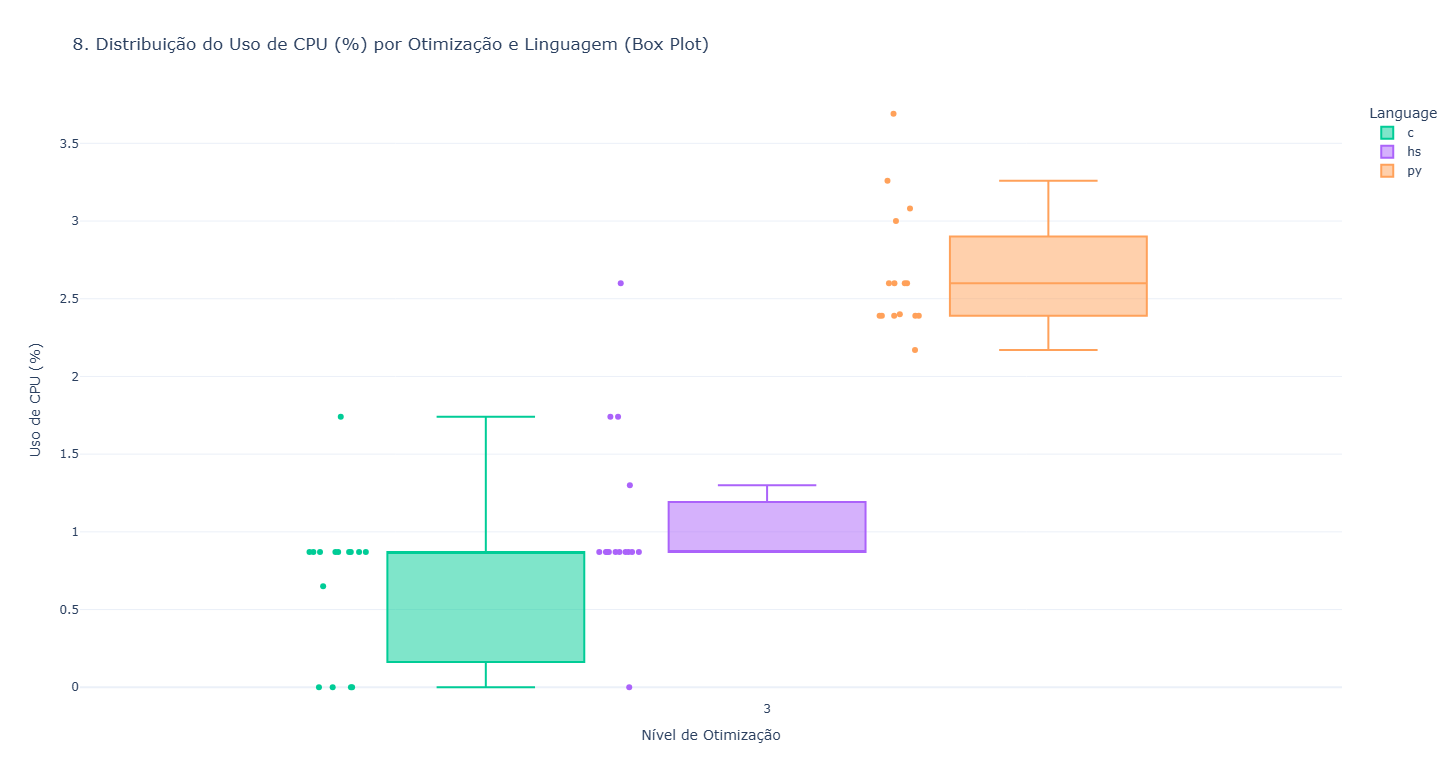
\includegraphics[width=1\textwidth]{Imagens/paradComp/mpf/cpu/boxplot_cpu_mpf.png}
    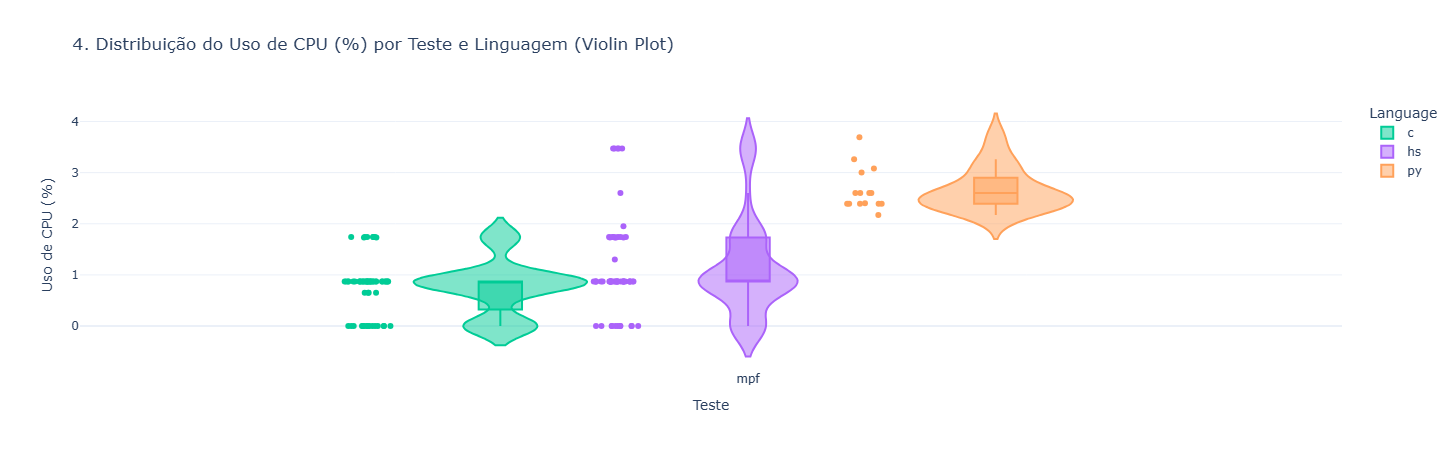
\includegraphics[width=1\textwidth]{Imagens/paradComp/mpf/cpu/violinplot_cpu_mpf.png}
    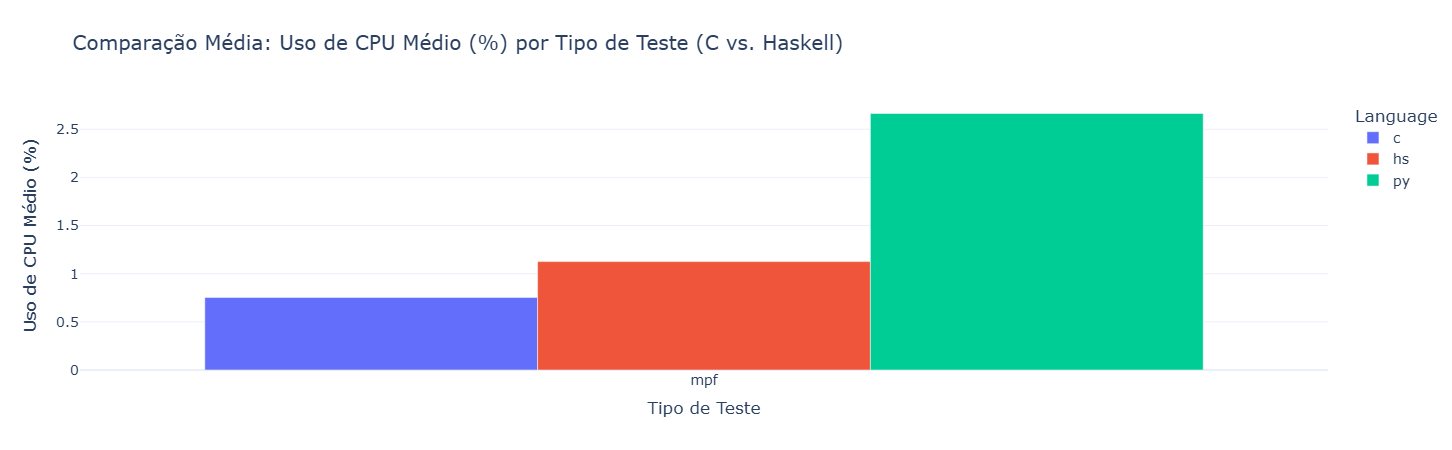
\includegraphics[width=1\textwidth]{Imagens/paradComp/mpf/cpu/mean_cpu_mpf.png}
    \caption{ Comparação do Uso de CPU entre Implementações Iterativa e Recursiva.}
    \label{fig: cpu_use_mpf}
\end{figure}

Os gráficos mostram uma melhor performance em relação ao uso de CPU de execução do C, seguido pelo Haskell e Python.

\begin{figure}[H]
    \centering 
    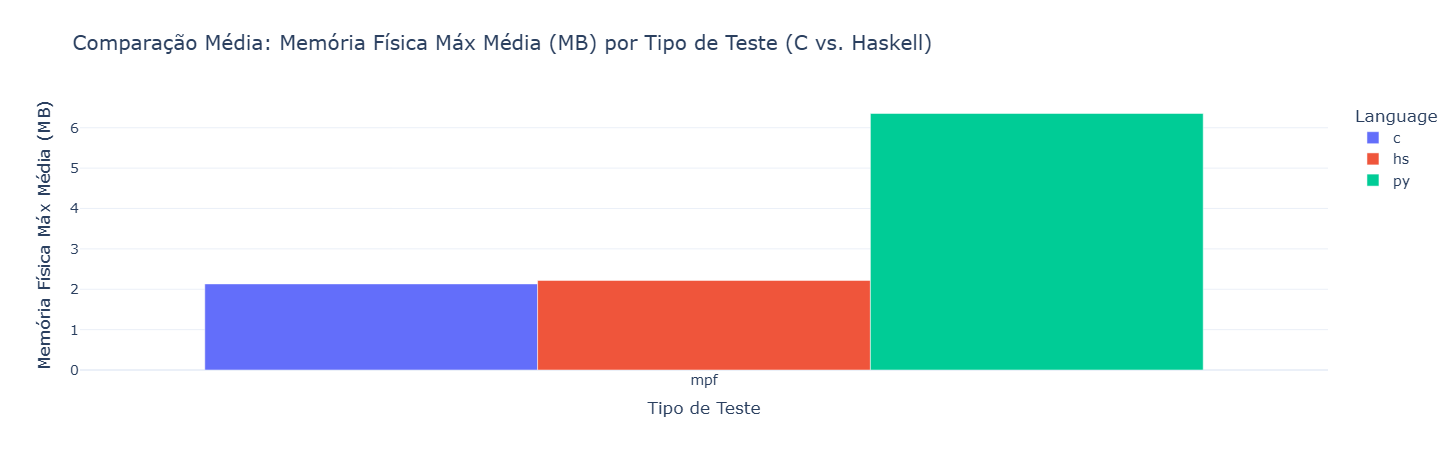
\includegraphics[width=1\textwidth]{Imagens/paradComp/mpf/mem/mean_memfis_mpf.png}
    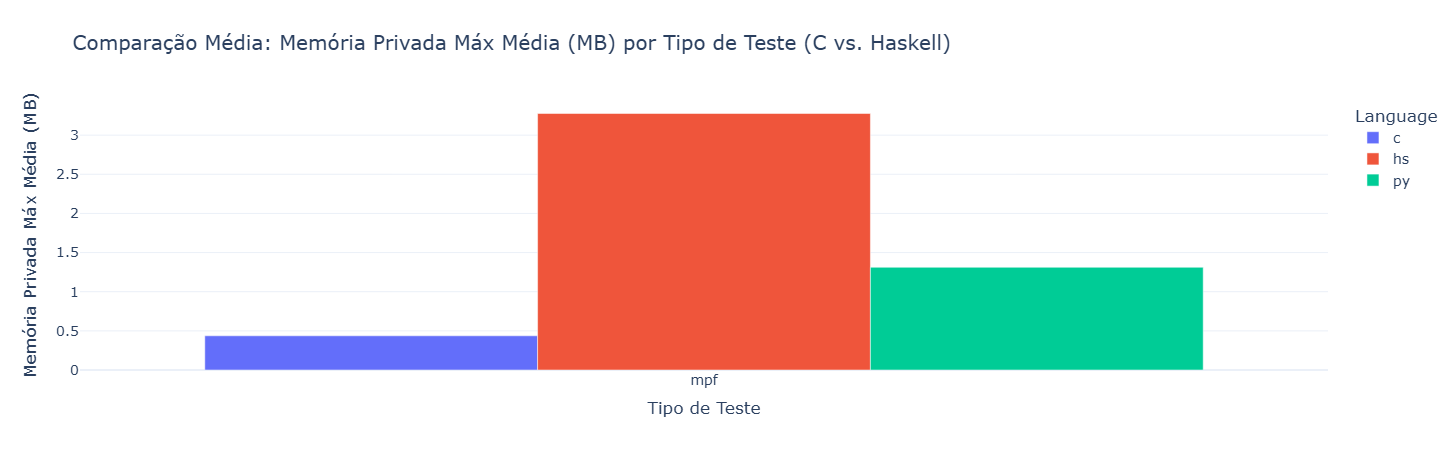
\includegraphics[width=1\textwidth]{Imagens/paradComp/mpf/mem/mean_mempriv_mpf.png}
    \caption{ Comparação do Uso de Memória entre Implementações Iterativa e Recursiva.}
    \label{fig: memory_use_mpf}
\end{figure}

O grafico de Memória Privada mostra o total de memória alocada para o processo, enquanto o gráfico de Memória Física mostra a quantidade de memória realmente utilizada durante a execução.
Em relação ao uso de memória, o C também apresentou a melhor performance, seguido pelo Python e Haskell.

\begin{figure}[H]
    \centering 
    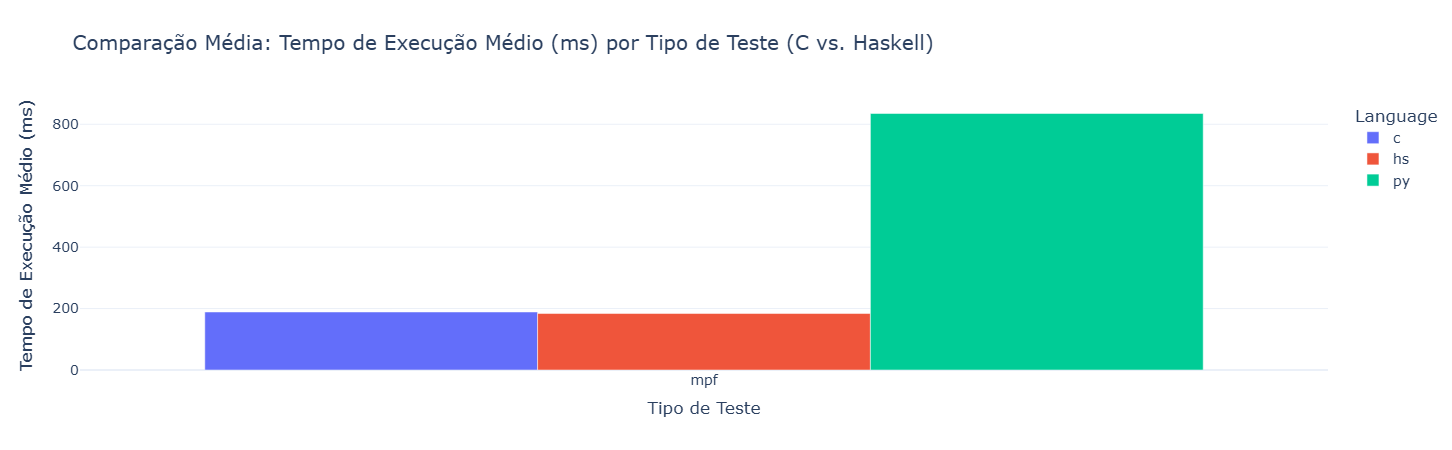
\includegraphics[width=1\textwidth]{Imagens/paradComp/mpf/time/mean_time_bar_nr.png}
    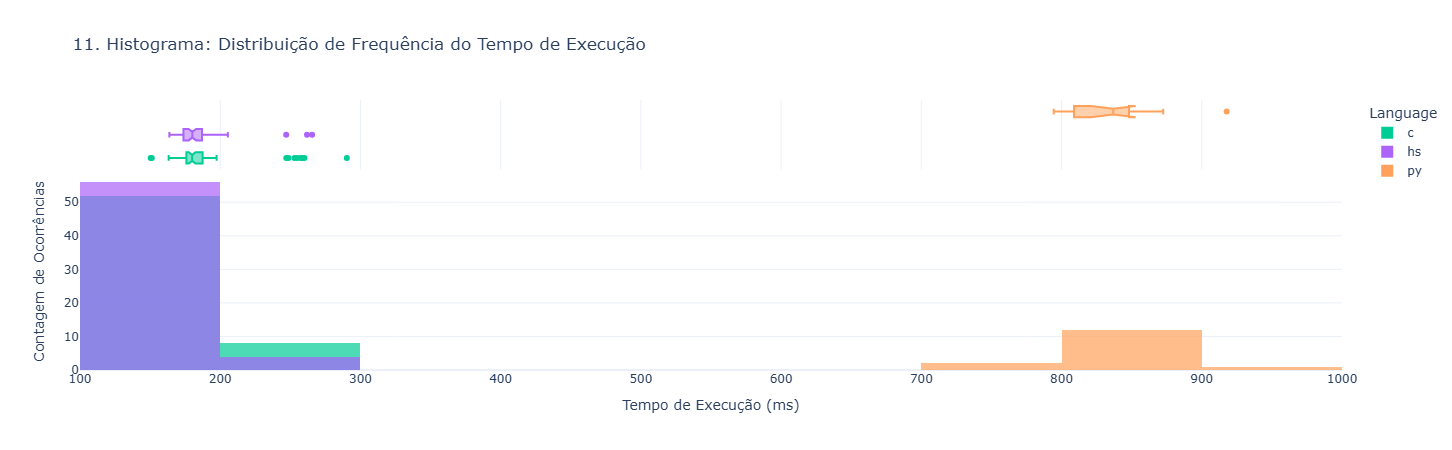
\includegraphics[width=1\textwidth]{Imagens/paradComp/mpf/time/time_hist_nr.png}
    \caption{ Comparação do Tempo de Execução entre Implementações Iterativa e Recursiva.}
    \label{fig: time_use_mpf}
\end{figure}

Em relação ao tempo de execução, o C novamente apresentou a melhor performance que foi muito parecida com a do Haskell. O Python por sua vez apresentou um desempenho muito pior em relação as outras linguagens.

\begin{figure}[H]
    \centering 
    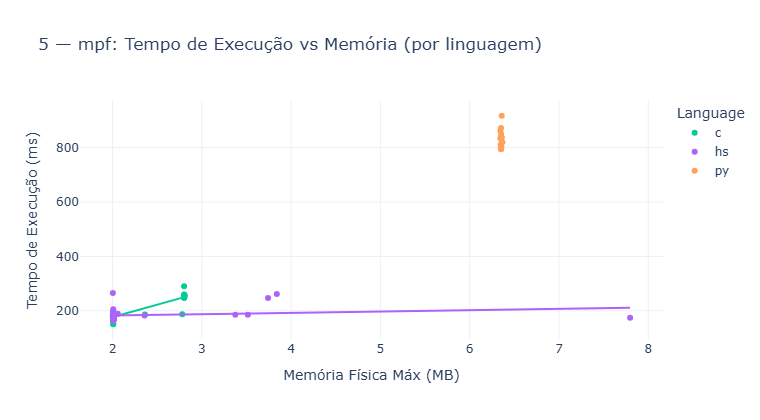
\includegraphics[width=1\textwidth]{Imagens/paradComp/mpf/time/trend/trend_langs_nr.png}
    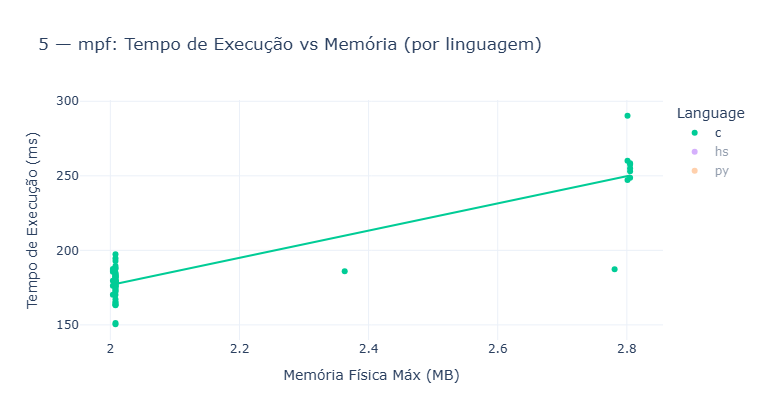
\includegraphics[width=1\textwidth]{Imagens/paradComp/mpf/time/trend/trend_c_nr.png}
    \caption{ Análise de Tendência do Tempo de Execução entre Implementações Iterativa e Recursiva. Parte 1}
    \label{fig: trend_time_use_mpf1}

\end{figure}
\begin{figure}[H]
    \centering 
    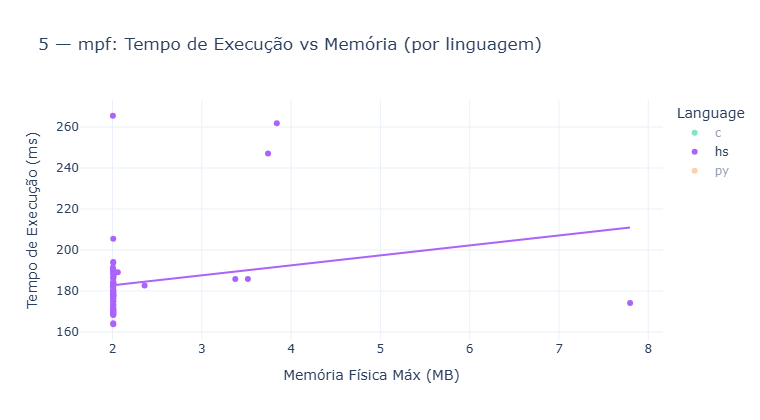
\includegraphics[width=1\textwidth]{Imagens/paradComp/mpf/time/trend/trend_hs_nr.png}
    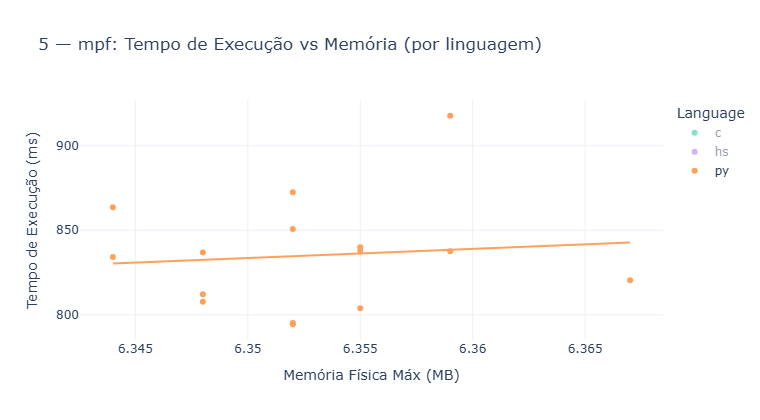
\includegraphics[width=1\textwidth]{Imagens/paradComp/mpf/time/trend/trend_py_nr.png}
    \caption{ Análise de Tendência do Tempo de Execução entre Implementações Iterativa e Recursiva. Parte 2}
    \label{fig: trend_time_use_mpf2}

\end{figure}

O gráfico de Trend mostra a tendencia do uso do tempo de execução em relação à memoria física utilizada. Podemos observar que o Python apresenta uma tendência mais estável. O Haskell apresenta uma tendência mais acentuada, enquanto o C apresenta uma tendência intermediária entre as duas.

Testes realizados no metódo de Newton-Raphson unidimensional foram coletados e analisados tanto iterativamente e recursivamente, vale ressaltar que a linguagem Haskell foi implementada apenas na forma recursiva, gerando os gráficos a seguir:

\begin{figure}[H]
    \centering 
    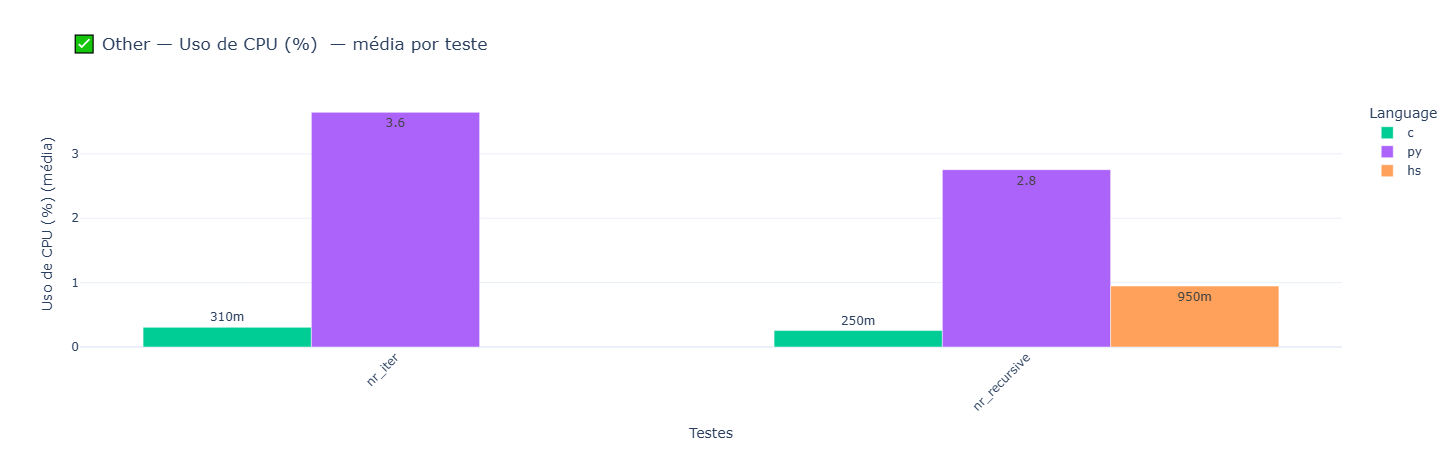
\includegraphics[width=1\textwidth]{Imagens/paradComp/nr/cpu/cpu_nr_hist_iter_vs_recursive_nr.png}
    \caption{ Comparação do Uso de CPU entre Implementações Iterativa e Recursiva.}
    \label{fig: cpu_use_hist_nr}
\end{figure}

Comparando o uso de CPU entre as implementações iterativa e recursiva, podemos observar que a implementação iterativa em C apresenta um desempenho muito superior em relação à implementação iterativa em Python. A implementação recursiva em Haskell, por sua vez, mostra um desempenho intermediário, ficando atrás do C, mas à frente do Python quando implementados recusivamente.
Comparando C e Python iterativamente e recursivamente, ambas tem o desempenho melhor na forma recursiva, gastando menos CPU, porém o C ainda é muito mais eficiente que o Python.


\begin{figure}[H]
    \centering 
    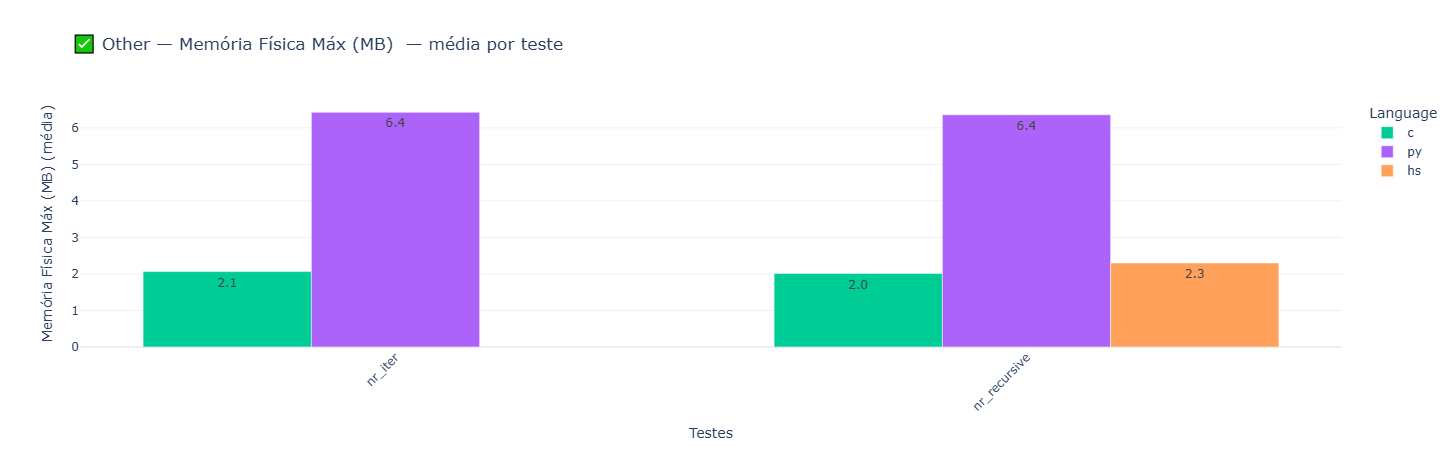
\includegraphics[width=1\textwidth]{Imagens/paradComp/nr/mem/fismem_nr_hist_iter_vs_recursive.png}
    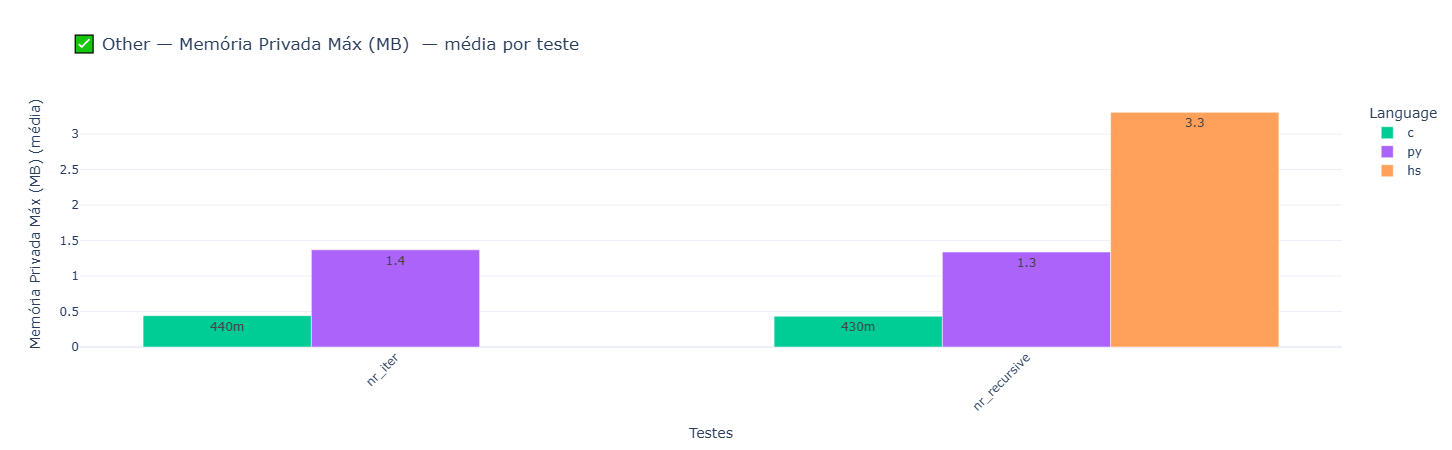
\includegraphics[width=1\textwidth]{Imagens/paradComp/nr/mem/privmem_nr_hist_iter_vs_recursive.png}
    \caption{ Comparação do Uso de Memória entre Implementações Iterativa e Recursiva.}
    \label{fig: memory_use_hist_nr}
\end{figure}

A analise da memória privada mostra que a implementação iterativa em C e python não mostraram muitas diferenças quando comparadas com suas contrapartes recursivas. Já a implementação recursiva em Haskell apresentou um uso de memória privada significativamente maior, o que pode ser atribuído à natureza da recursão e à forma como o Haskell gerencia a memória para chamadas de função recursivas.

Já a memória física utilizada mostrou que a implementação iterativa em C utilizou levemente menos memória física em comparação com a implementação recursiva. A implementação iterativa em Python, por outro lado, utilizou uma quantidade de memória física que não se alterou mas foi muito maior do que ambas outras linguagens nas duas implementações, tanto iterativa quanto recursiva.

\begin{figure}[H]
    \centering 
    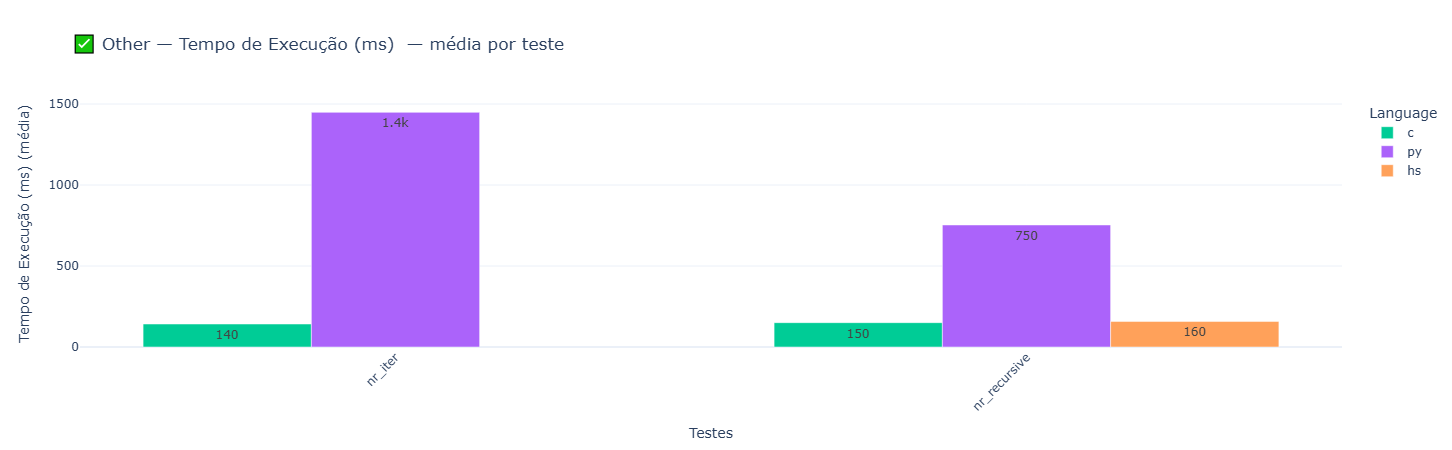
\includegraphics[width=1\textwidth]{Imagens/paradComp/nr/time/time_nr_hist_iter_vs_recursive.png}
    \caption{ Comparação do Tempo de Execução entre Implementações Iterativa e Recursiva.}
    \label{fig: time_use_hist_nr}
\end{figure}

O tempo de execução mostra que a implementação iterativa em C foi a mais rápida, seguida pela implementação recursiva em C que por sua vez é seguida da implementação em Haskell. A implementação iterativa em Python foi a mais lenta entre as três, mas ainda assim apresentou um desempenho muito melhor quando é implementada recursivamente.


\begin{figure}[H]
    \centering 
    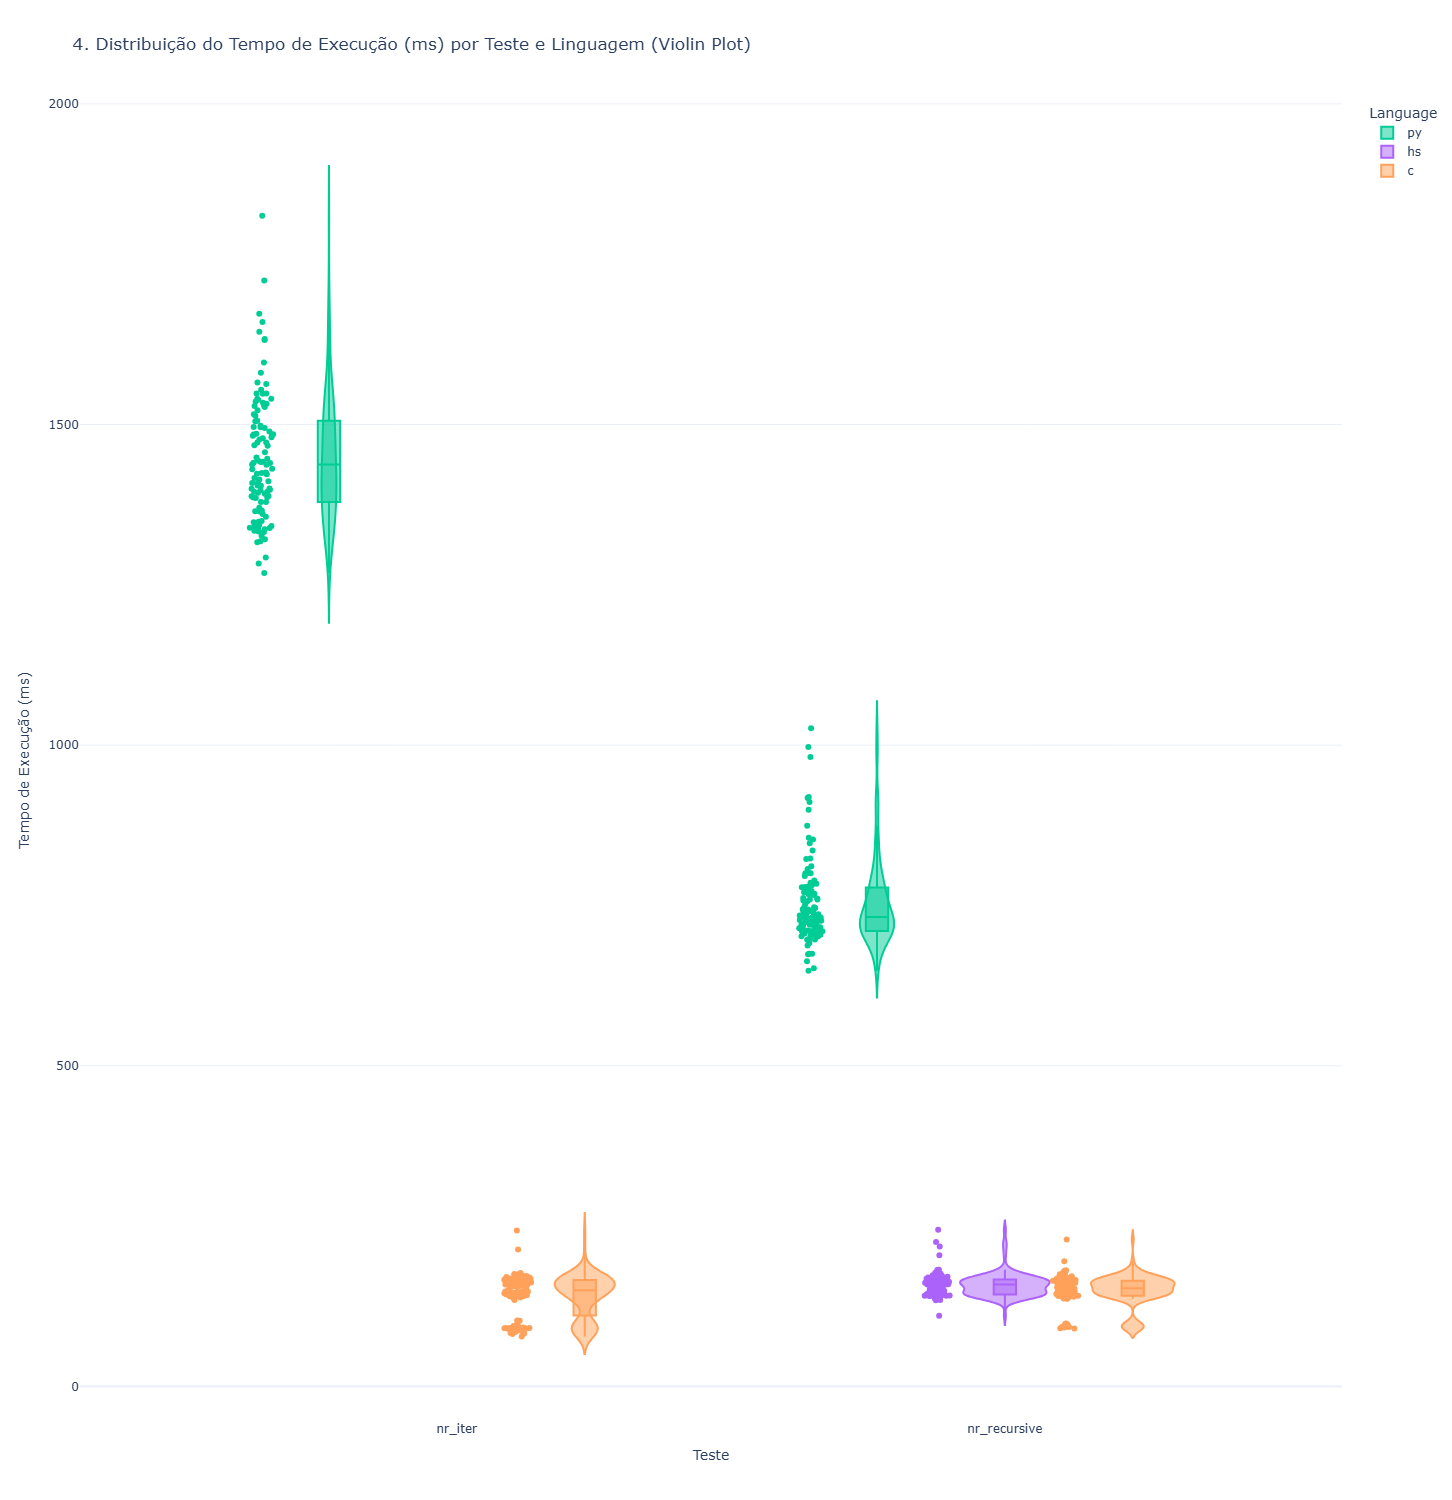
\includegraphics[width=1\textwidth]{Imagens/paradComp/nr/time/time_nr_violin_iter_vs_recursive.png}
    \caption{ Violin Plot do Tempo de Execução entre Implementações Iterativa e Recursiva.}
    \label{fig: time_use_violin_nr}
\end{figure}

\begin{figure}[H]
    \centering 
    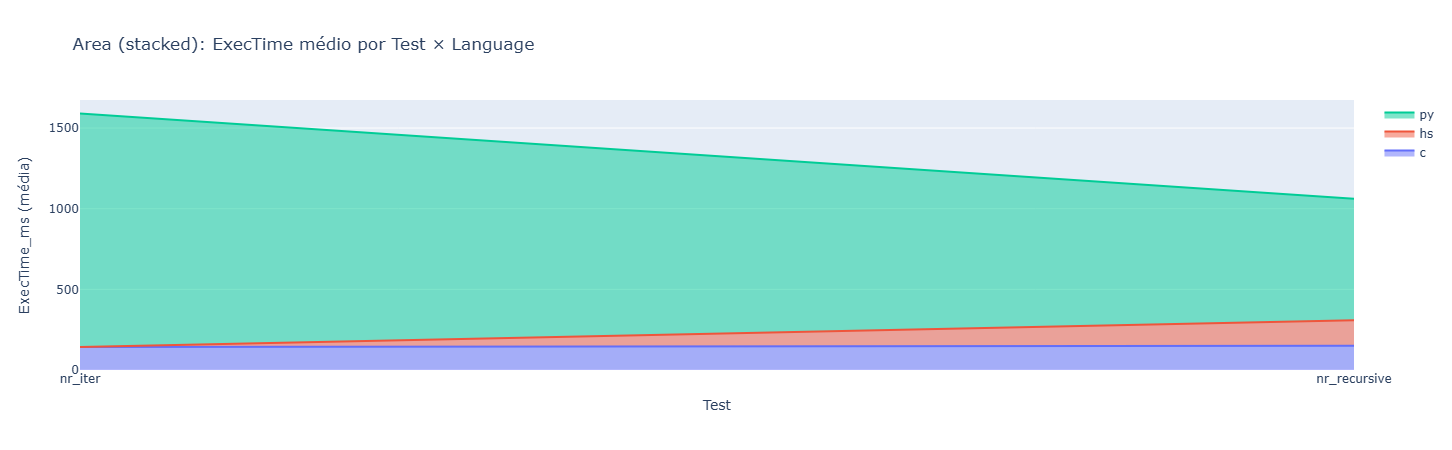
\includegraphics[width=1\textwidth]{Imagens/paradComp/nr/stacked.png}
    \caption{ Gráfico Empilhado do Tempo de Execução entre Implementações Iterativa e Recursiva. }
    \label{fig: time_dist_per_lang_nr}
\end{figure}


Ambos os graficos de Violin Plot e Área Empilhada reforçam a análise anterior, mostrando claramente a superioridade do C em termos de tempo de execução, seguido pelo Haskell e Python. Apesar disso, na implementação recursiva, o Haskell mostrou-se ligeramente mais estável do que o C. O python por sua vez apresentou uma variação maior no tempo de execução em ambas implementações, mas a recursiva ainda melhor que a iterativa.


\begin{figure}[H]
    \centering
    \makebox[\textwidth][c]{%
        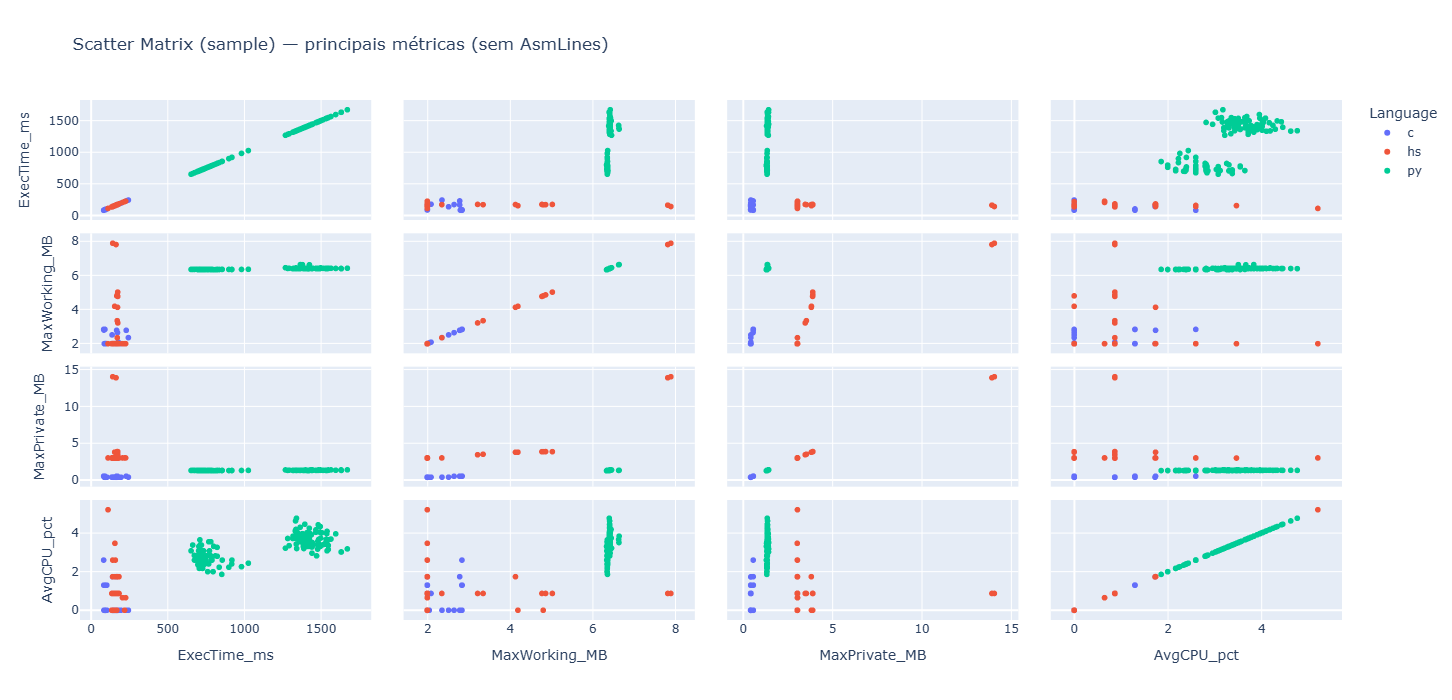
\includegraphics[width=1.15\textwidth]{Imagens/paradComp/nr/scatterMatrix_nr.png}%
    }
    \caption{Matriz de Dispersão das Métricas Coletadas.}
    \label{fig: scatterMatrix_nr}
\end{figure}

A matriz de dispersão das métricas coletadas oferece uma visão abrangente das relações entre diferentes variáveis, como uso de CPU, memória física, memória privada e tempo de execução. Observa-se que há correlações positivas entre o uso de CPU e o tempo de execução, indicando que implementações que consomem mais CPU tendem a levar mais tempo para completar.


\backmatter

\nocite{*}

\bibliographystyle{plain}
\bibliography{Capitulos/ref}
\end{document}
